\documentclass[a4paper]{scrartcl}
\usepackage{subcaption}
\usepackage[english]{babel}
\usepackage[utf8]{inputenc}
\usepackage{amsmath}
\usepackage{graphicx}
\usepackage[colorinlistoftodos]{todonotes}
\usepackage{authblk}
\usepackage{lineno}
\usepackage{cite}
\usepackage{amsmath}
\usepackage{url}
\usepackage{booktabs}
\def\mymathhyphen{{\hbox{-}}}
\linenumbers
\addtokomafont{disposition}{\rmfamily}
\usepackage{appendix}
\usepackage{hyperref}

\renewcommand{\arraystretch}{1.2}
\newcommand{\ra}[1]{\renewcommand{\arraystretch}{#1}}

\title{Reconstruction Efficiencies for Data \& MC using the Muon Counter System \\ \vspace{1em} \small{\textbf{MICROBOONE-NOTE-XXXX-INT-vX}}}

\author[1]{M. Bass\thanks{matthew.bass@physics.ox.ac.uk}}
\author[1]{R. Guenette\thanks{roxanne.guenette@physics.ox.ac.uk}}
\author[1]{S.R. Soleti\thanks{stefano.soleti@physics.ox.ac.uk}}
\affil[1]{\emph{\small{University of Oxford, Oxford OX1 3RH, United Kingdom}}}

\date{\today}

\begin{document}
\maketitle

\setcounter{section}{-1}

\section{Purpose of Forthcoming Public Note}

The message of the public note based upon this document is as follows:

\begin{itemize}
  \item reconstructed tracks in the TPC can be matched to hits in an external cosmic ray counter (in our case the MuCS);
  \item the data reconstruction efficiency can be measured comparing the number of MuCS-triggered events with the number of MuCS reconstructed tracks;
  \item there is a systematic error in the measurement of the data reconstructing efficiency due to the presence of detector non-uniformities;
  \item the multiple scattering of the cosmic rays introduces an irreducible impurity in our sample of MuCS reconstructed tracks.
  \item taking into account these systematic effects, the data reconstruction efficiency obtained with the MuCS is in agreement with a Monte Carlo reconstruction efficiency generated uniformly across the TPC.

\end{itemize}

The figures that will be carried forward to the public note are Figg. \ref{fig:mucs}, \ref{fig:3dmipcut}, \ref{fig:res} (\texttt{pandoraCosmic} only), \ref{fig:pandora_3D}-\ref{fig:pandora_3D_mc}, \ref{fig:2d_pc1}-\ref{fig:2d_pc1_mc}-\ref{fig:2d_pc2}-\ref{fig:2d_pc2_mc}-\ref{fig:2d_pc3}-\ref{fig:2d_pc3_mc}, \ref{fig:xy}-\ref{fig:yz}-\ref{fig:l}  (\texttt{pandoraCosmic} only), \ref{fig:ineff}, \ref{fig:cry_mc_3d}, \ref{fig:cry_mc_2d}, \ref{fig:cry_mc_2d_2}, \ref{fig:cry_mc_2d_3}, \ref{fig:cry_mc_1d}, \ref{fig:plans} and \ref{fig:500mev1d}.

\section{Introduction}
This analysis note describes the work done to study the reconstruction efficiencies using a dataset of cosmic rays passing through the Muon Counter System (MuCS).
The goal is to provide data and Monte Carlo reconstruction efficiencies that can be used to compare reconstruction performances and to show that an external cosmic-ray counter can be used to measure the data reconstruction efficiency in the LArTPC.

We measured the data reconstruction efficiency comparing the number of events triggered by the MuCS and the number of events with a MuCS-compatible reconstructed track.
The Monte Carlo reconstruction efficiency, instead, was measured by comparing the number of generated cosmic rays with the number of reconstructed tracks.

The reconstruction efficiency is expressed as a function of the cosmic-ray starting angle (given by the spherical angles $\theta$ and $\phi$) and of the expected length $L$ of its path in the TPC, assuming it is a minimum-ionizing particle (MIP).

Using the \texttt{pan\-do\-ra\-Co\-smic} algorithm \cite{pandoracosmic} provided by the Pandora framework \cite{pandora}, the overall reconstruction efficiency is $96.1\pm0.1\thinspace(\mathrm{stat}) \pm 1.1\thinspace(\mathrm{sys})\thinspace\%$ for data and $96.3\pm0.1\thinspace\%$ for Monte Carlo.

In the future, the method described in this paper will be adapted to use the data coming form the Cosmic Ray Tagger \cite{crt}, which is able to tag around 80\% of the cosmic rays hitting MicroBooNE LArTPC. In this way, we will be able to cover the entire $(\theta,\phi,L)$ parameter space and measure efficiency-corrected quantities, such as the cosmic-ray flux in the LArTPC.

\section{The Muon Counter System}\label{sec:proc}
The MuCS consists of two sets of planar modules made up of scintillator strips placed into two separate, light-tight boxes, readout via wavelength shifting fibers connected to Multi-Anode PMTs and placed on the top of the TPC. The Multi-Anode PMTs are readout by a DAQ system, separated from the DAQ system that reads out the TPC and PMT systems of the main detector.

Each planar module is made up of two sets of 24 scintillator strips, 4 cm wide, arranged into bi-layers oriented perpendicular to each other. This configuration provides two coordinates ($z$ and $x$ in the MicroBooNE TPC coordinate system, shown in Fig. \ref{fig:coord}) of the crossing points of the cosmic rays. Combining these two coordinates with the height of the modules (corresponding to the $y$ coordinate in the MicroBooNE TPC coordinate system), it is possible to extrapolate the three-dimensional trajectory of the cosmic ray.

The starting angle of the cosmic ray, in spherical coordinates, will be given by:
\begin{align}
  \theta_{\mathrm{MuCS}} = \mathrm{acos}\left(\frac{z_{\mathrm{top}}-z_{\mathrm{bottom}}}{r}\right) \\
  \phi_{\mathrm{MuCS}} = \mathrm{atan}\left(\frac{y_{\mathrm{top}}-y_{\mathrm{bottom}}}{x_{\mathrm{top}}-x_{\mathrm{bottom}}}\right),
\end{align}
where $r = \sqrt{(x_{\mathrm{top}}-x_{\mathrm{bottom}})^2+(y_{\mathrm{top}}-y_{\mathrm{bottom}})^2+(z_{\mathrm{top}}-z_{\mathrm{bottom}})^2}$ and the top (bottom) coordinates are given by the hits in the top (bottom) MuCS panel.
\begin{figure}[htbp]
  \begin{center}
    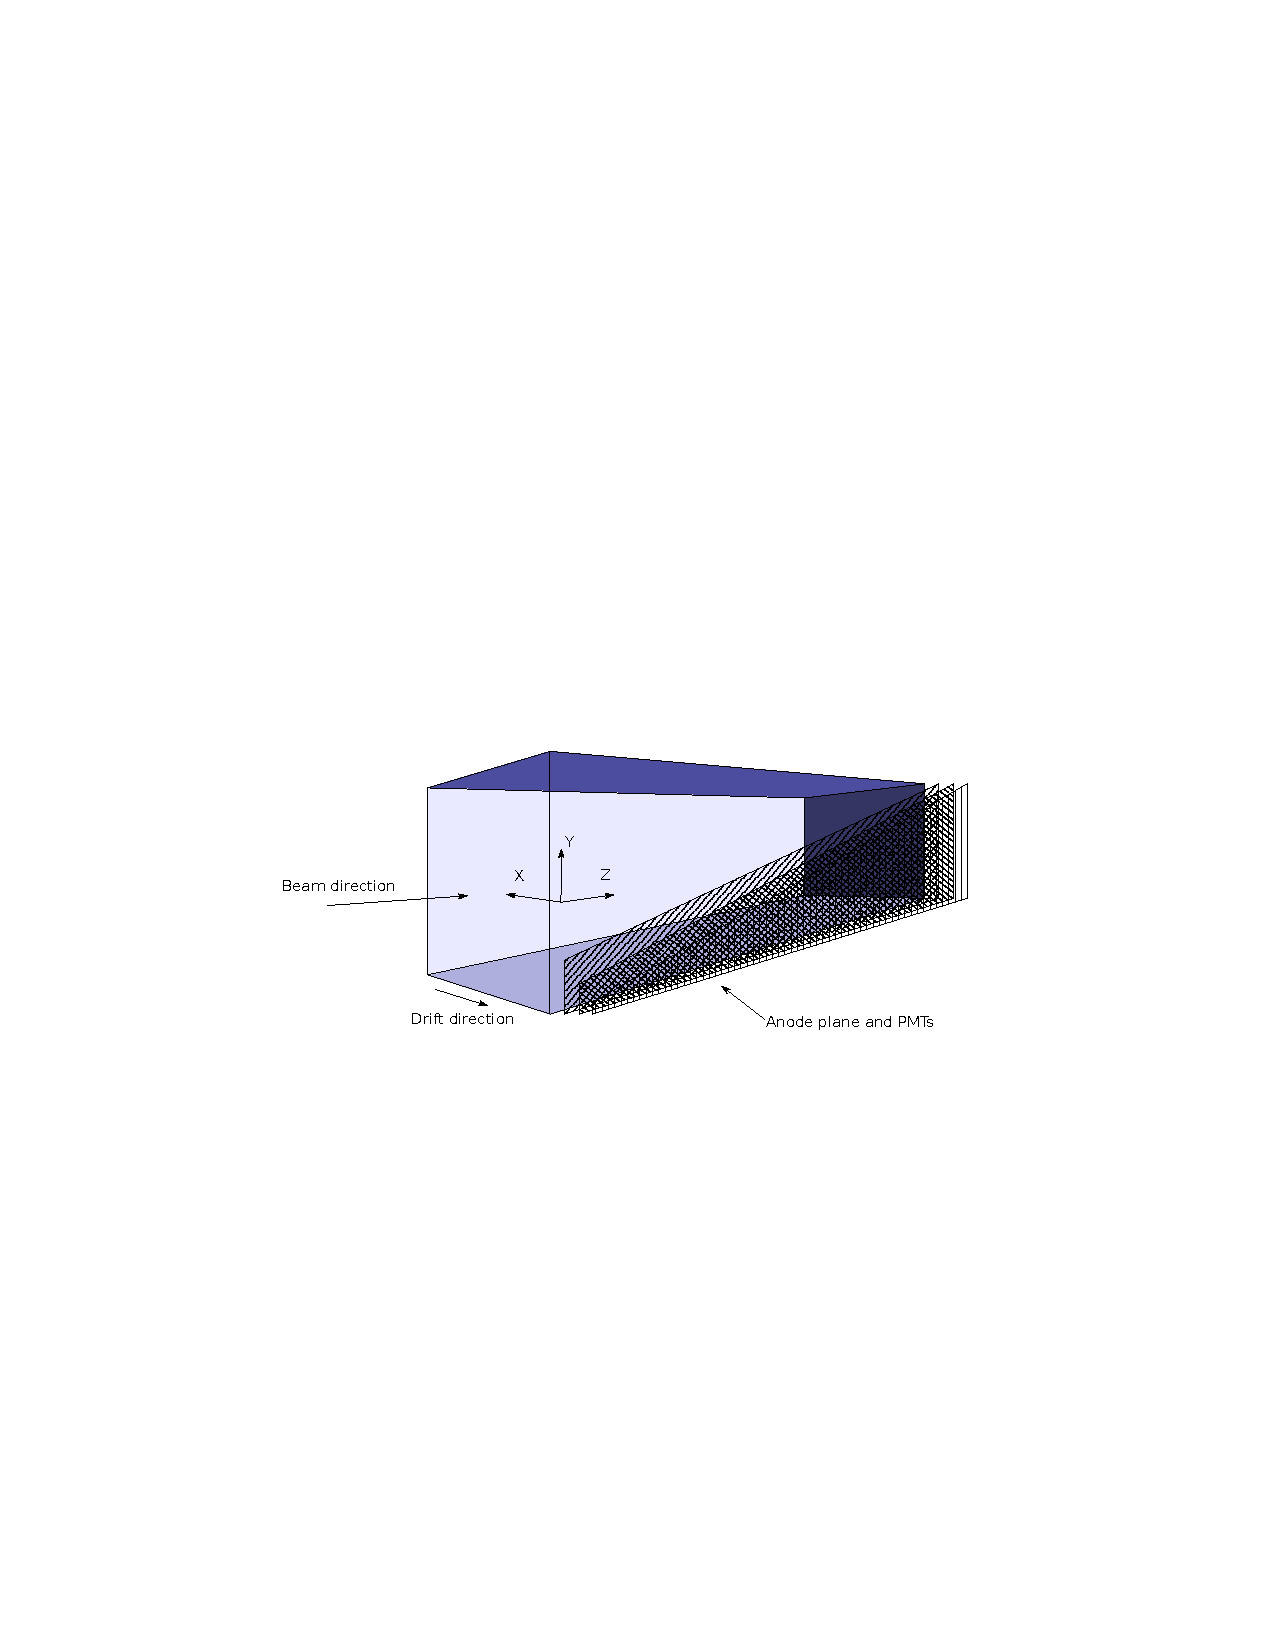
\includegraphics[width=0.8\linewidth]{figures/coord.pdf}

    \caption{The MicroBooNE coordinate system. The three wire planes are vertical (collection plane) and at  $\pm60^{\circ}$ to the vertical (induction planes). The dimensions of the TPC are 256.35 cm $\times$ 233 cm $\times$ 1036.8 cm (x $\times$ y $\times$ z). The fiducial volume of the detector is 236.35 cm $\times$ 203 cm $\times$ 1026.8 cm. The coordinate system is explained in detail in \cite{mcdata}} \label{fig:coord}
  \end{center}
\end{figure}

This analysis has been performed on three merged dataset, acquired with different geometrical configurations. In each configuration, the two boxes have been placed at the upstream end, at the center and at the downstream end of the LArTPC, respectively.

A three-dimensional schematics of the three MuCS setups is shown in Fig. \ref{fig:mucs} and the coordinates of the two boxes for each configuration are reported in Tab. \ref{tab:mucs}.
\begin{figure}[htbp]
  \begin{subfigure}{0.30\textwidth}
    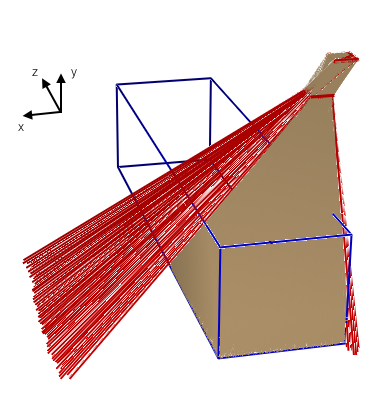
\includegraphics[width=\linewidth]{figures/upstream.png}
    \caption{Upstream} \label{fig:upstream}
  \end{subfigure}
  \begin{subfigure}{0.30\textwidth}
    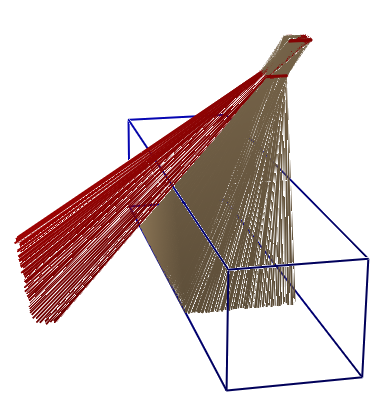
\includegraphics[width=\linewidth]{figures/center.png}
    \caption{Center} \label{fig:centre}
  \end{subfigure}
  \begin{subfigure}{0.30\textwidth}
    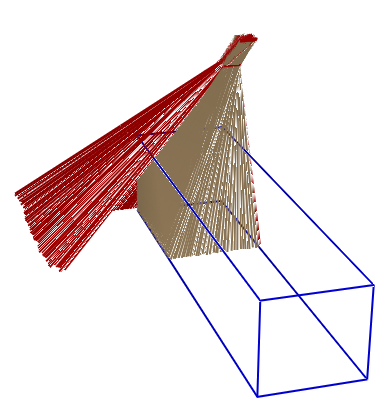
\includegraphics[width=\linewidth]{figures/downstream.png}
    \caption{Downstream} \label{fig:downstream}
  \end{subfigure}

  \caption{Monte Carlo simulation of the possible MuCS trajectories the three different MuCS setups used in this analysis. Brown tracks correspond to cosmic rays hitting both panels and the TPC, while red tracks go through the MuCS but miss the TPC.} \label{fig:mucs}
\end{figure}

\begin{table}[htbp]
  \centering
  \ra{1.2}
  \begin{tabular}{lcrrrccccc}
    \toprule
    \textbf{Box} & \phantom{abc}& \multicolumn{2}{c}{x [cm]} & \phantom{abc} & \multicolumn{2}{c}{y [cm]} & \phantom{abc} & \multicolumn{2}{c}{z [cm]}\\
    \cmidrule{3-4} \cmidrule{6-7} \cmidrule{9-10}
    & & start & end & & start & end & & start & end\\
    \midrule

    \textbf{Upstream} & & & & & & & & & \\
    Top box & & -75 & -27 & & 392 & 393 & & 224 & 272\\
    Bottom box & & -27 & 21 & & 320 & 321 & & 224 & 272\\

    \midrule
    \textbf{Center} & & & & & & & & & \\
    Top box & & -72 & -24 & & 397 & 398 & & 579 & 627\\
    Bottom box & & -27 & 21 & & 320 & 321 & & 581 & 629\\
    \midrule
    \textbf{Downstream} & & & & & & & & & \\
    Top box & & -75 & -27 & & 392 & 393 & & 971 & 1019\\
    Bottom box & & -27 & 21 & & 320 & 321 & & 971 & 1019\\
    \bottomrule

  \end{tabular}
  \caption{Coordinates of the top and bottom box of the MuCS detector for three geometrical setups.}\label{tab:mucs}
\end{table}


\section{MuCS merging}\label{sec:merging}
The MuCS is designed to provide a trigger on through-going muons that intersect two planes of scintillator strips. The trigger is propagated to the MicroBooNE trigger system to record a full TPC and PMT readout. With the MuCS trigger in place, the $t_0$ for a track associated with the MuCS is known and these tracks are useful for various detector physics and reconstruction studies.

The dataset used for this study has been collected with the DAQ configured in the trigger-readout mode: the MuCS trigger is sent to the TPC readout, while the MuCS DAQ saves the hit patterns seen in the scintillator strips.
The MuCS triggers at a rate of nearly 3 Hz and this rate is prescaled by 100 before sending the signal to trigger readout. In the general data stream then, a MuCS trigger is issued at a rate of 0.02 Hz (lower than 0.03 Hz because the MuCS trigger is often vetoed by beam triggers), or roughly one per minute.
Given a DAQ integration window of 100 ns, the accidental coincidental rate is negligible for our study. The probability that, during the same readout window (4.8 ms), another cosmic ray hits the MuCS is, given a trigger rate of 3 Hz, 0.01\% and it has also been considered negligible.

The data then follows a processing path that merges the MuCS hit patterns and reconstructed trajectory information with the TPC and PMT data stream to form a MuCS-merged dataset. A flowchart of the procedure is shown in Fig. \ref{fig:scheme}.

\begin{figure}[htbp]
  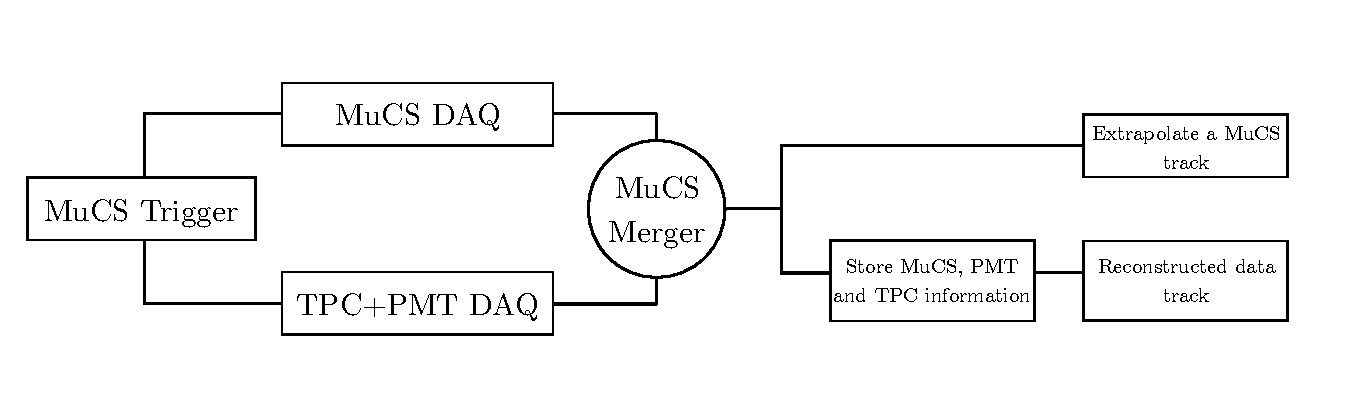
\includegraphics[width=\linewidth]{figures/scheme.pdf}
  \caption{Flowchart showing the procedure used to generate the dataset used in this analysis. We end up with two data products: one with extrapolated coordinates obtained using MuCS-only data and one with reconstructed data information.} \label{fig:scheme}
\end{figure}

The hits in the MuCS are used to obtain a bi-dimensional point in each panel and extrapolate a three-dimensional track (MuCS-extrapolated track). The TPC hits, instead, are fed to the reconstruction chain: then, the reconstructed track with the closest starting point (within a tolerance) to the MuCS-extrapolated track is stored in the dataset and it is tagged as a MuCS-reconstructed track. The PMT flash in time with the MuCS signal, if present, is also stored and associated to the MuCS-reconstructed track.  Fig. \ref{fig:evd} shows a diagram with the MuCS-reconstructed track, the MuCS-extrapolated track and the other reconstructed tracks in the same readout window.
\begin{figure}[htbp]
  \begin{center}
  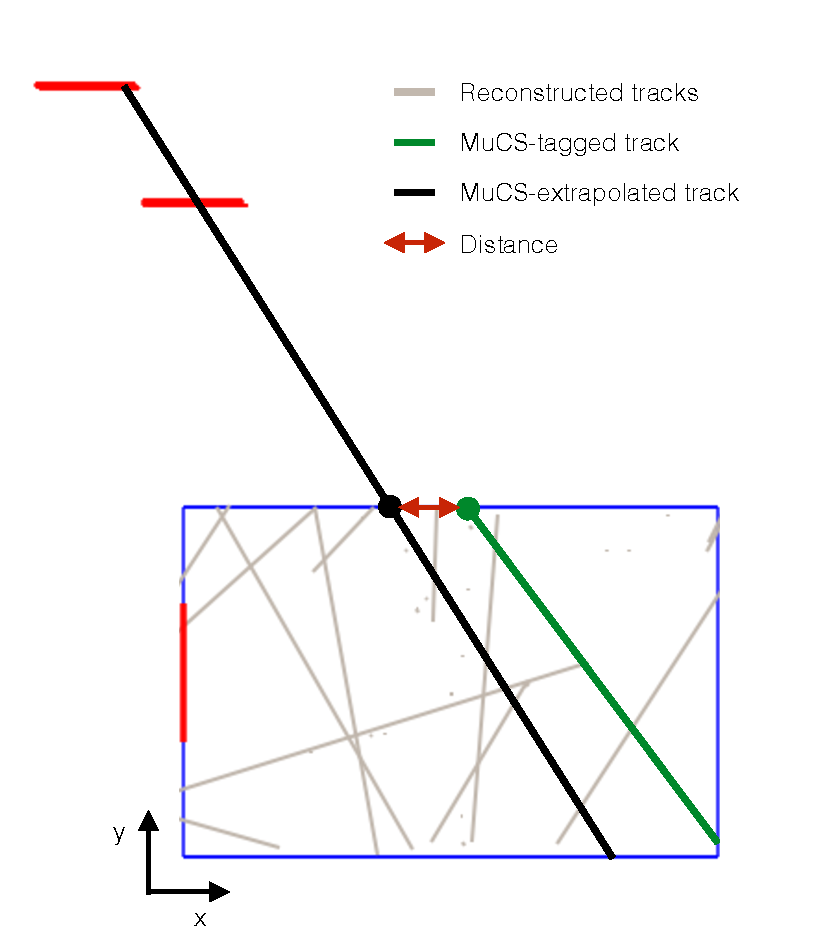
\includegraphics[width=0.50\linewidth]{figures/evd.pdf}  \vspace{1.8em}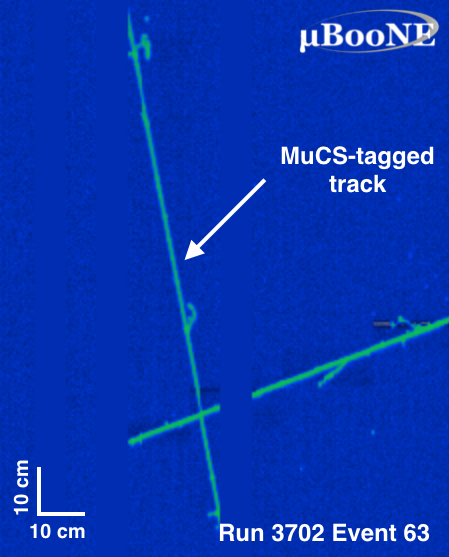
\includegraphics[width=0.40\linewidth]{figures/evd_display.png}

  \caption{Left: bi-dimensional view of a MuCS event. The black line shows the MuCS-extrapolated tracks, while the green line correspond to the MuCS-reconstructed track. Right: corresponding portion of the event display for the collection plane, showing the MuCS-reconstructed track. } \label{fig:evd}
\end{center}
\end{figure}
Our dataset will then include two different sets of information, with a one-to-one correspondence:
\begin{itemize}
  \item MuCS-extrapolated information: using the two 2D points given by the MuCS (one for each box) we extrapolate a 3D line crossing the entire TPC. In this way we obtain two extrapolated starting angles ($\theta$ and $\phi$), an extrapolated track length $L$ and extrapolated start/end points, using only MuCS information.
  \item Reconstructed TPC data information: for each event, we store the reconstructed spatial information of the MuCS-reconstructed track and of the in-time PMT flash, if present.
\end{itemize}


As Monte Carlo sample we used a complete cosmic-ray simulation, as described in \cite{cosmic}. The cosmic rays have ben generated using CORSIKA \cite{corsika},  propagated using GEANT4 \cite{geant}, and then passed through the detector simulation stage. The detector simulation attempts to simulate the detector response as precisely as possible, meaning that the current state of the detector is reflected, including known missing wires. Other known effects, such as the space charge effect \cite{sce}, are not currently modeled in the simulation.

From this complete Monte Carlo simulation, then, we selected only the cosmic rays with a starting angle $(\theta,\phi)$ within the geometrical acceptance of the MuCS.

Our aim is to show that the reconstruction efficiency of simulated cosmic rays, generated all over the TPC, can be successfully compared to the data reconstruction efficiency, obtained placing a small muon counter system in three different places.

\section{MuCS-triggered cosmic rays angular distributions}\label{sec:flux}
Before measuring the reconstruction efficiency we performed a survey of the position of the MuCS panels in each configuration. Taking the starting point and starting direction of the MuCS-reconstructed tracks it is possible to extrapolate their trajectory up to the height of the boxes and check if they went through both panels. However, the build-up of positive argon ions in the TPC causes a distortion in the electric field and consequently in the reconstruction of the tracks. Thus, before measuring the starting angles and extrapolating the paths, the starting position and direction of the reconstructed tracks in the TPC have been corrected with the data-driven procedure described in \cite{sce}.

The two-dimensional plots of the extrapolated positions are reported in Fig. \ref{fig:alignment}. As we can see, some tracks are extrapolated outside the panels, because of multiple Coulomb scattering, but the majority of the points are well within the panels' borders.

\begin{figure}[htbp]
  \begin{subfigure}{0.32\textwidth}
    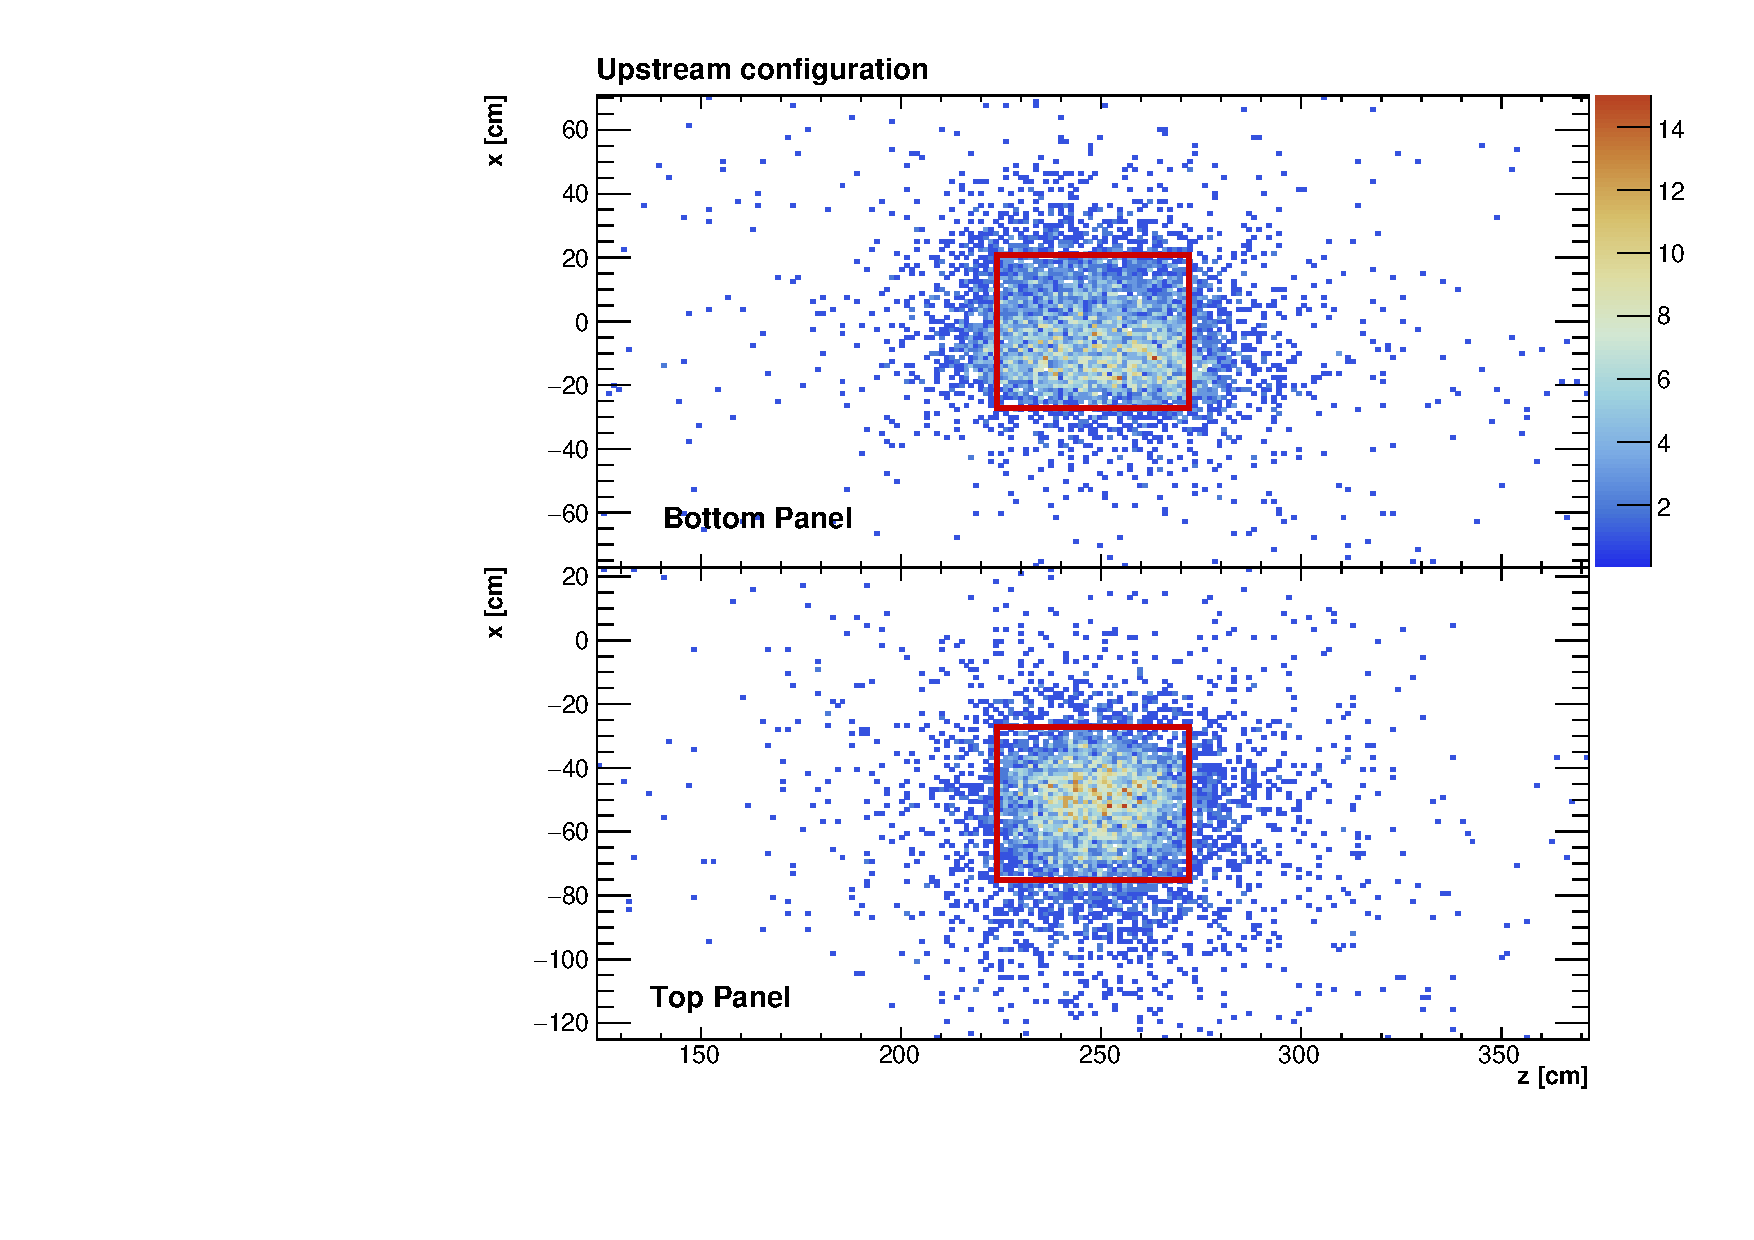
\includegraphics[width=\linewidth]{figures/upstream.pdf}
    \caption{Upstream} \label{fig:upstream_align}
  \end{subfigure}
  \begin{subfigure}{0.32\textwidth}
    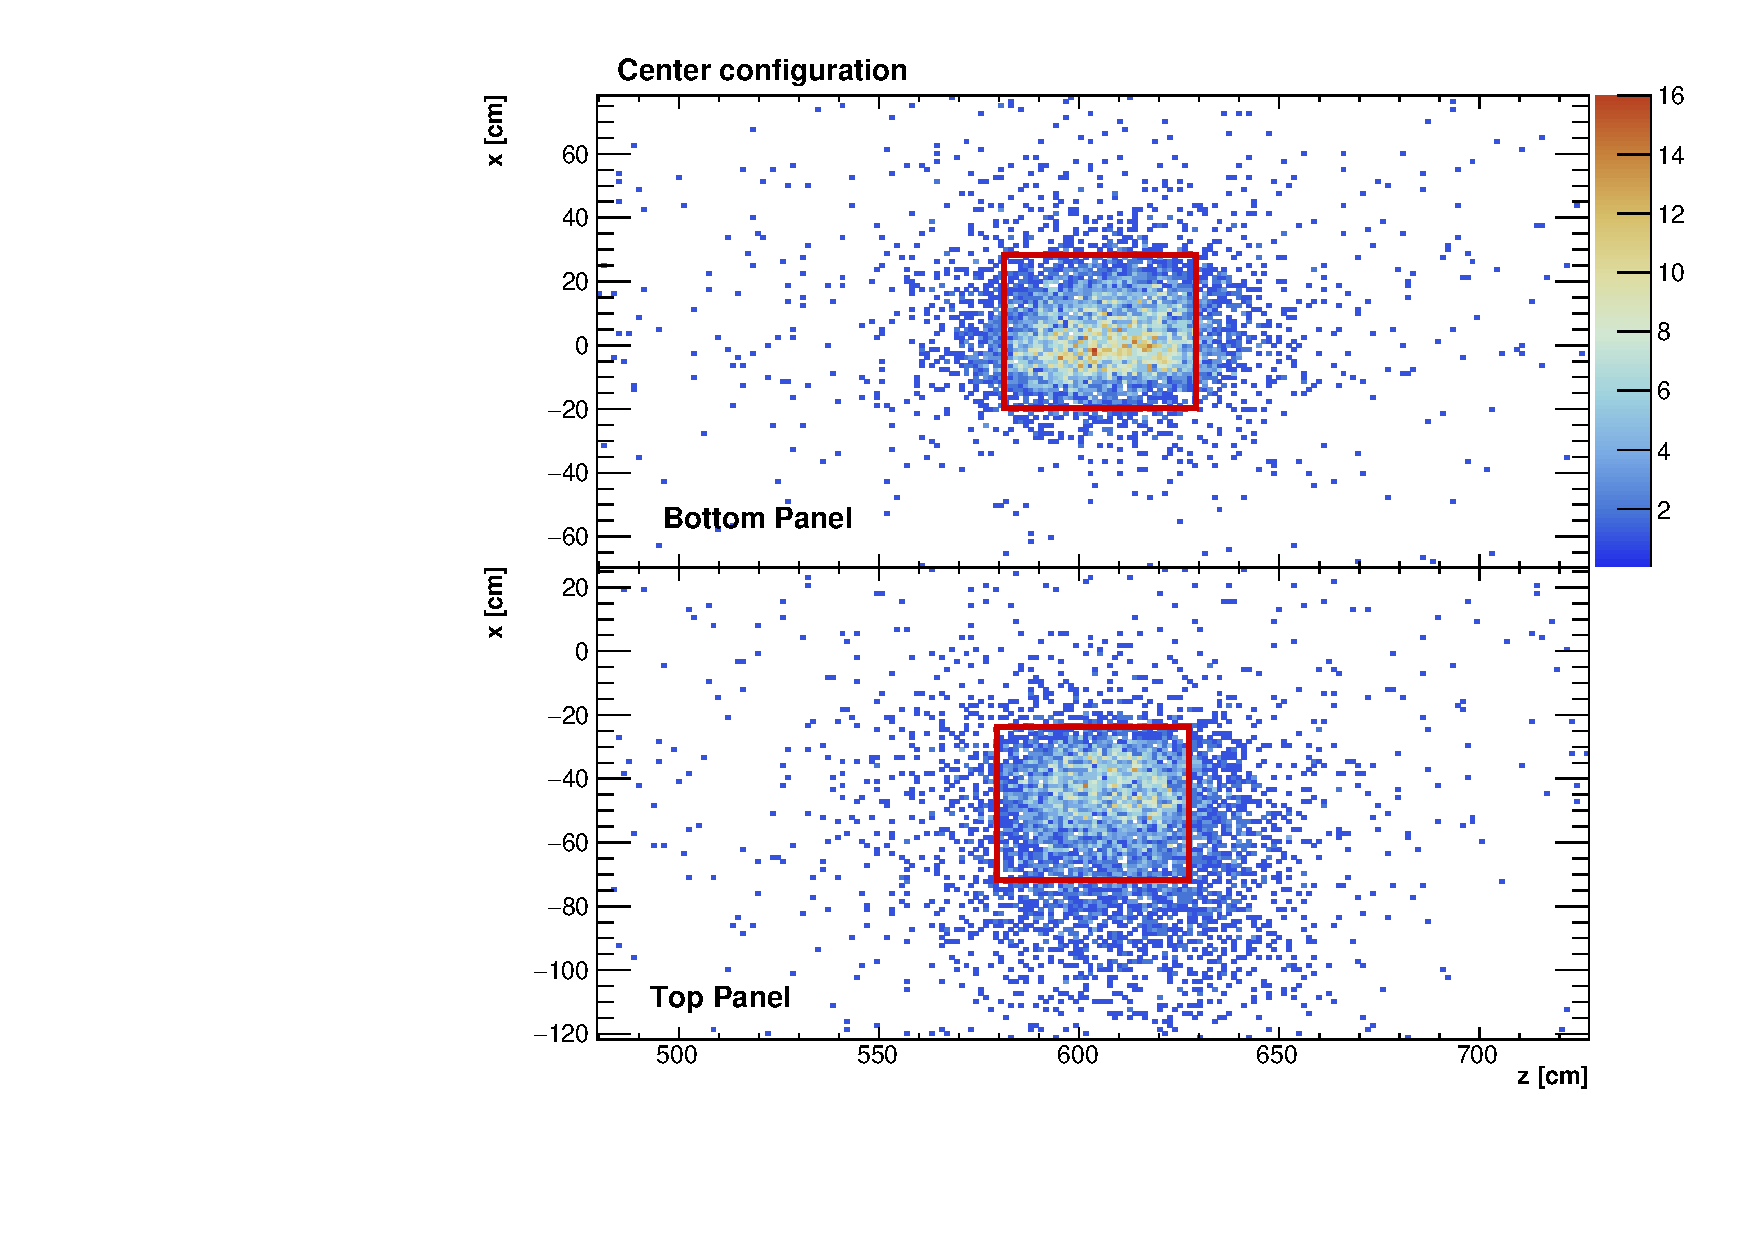
\includegraphics[width=\linewidth]{figures/centre.pdf}
    \caption{Center} \label{fig:centre_align}
  \end{subfigure}
  \begin{subfigure}{0.32\textwidth}
    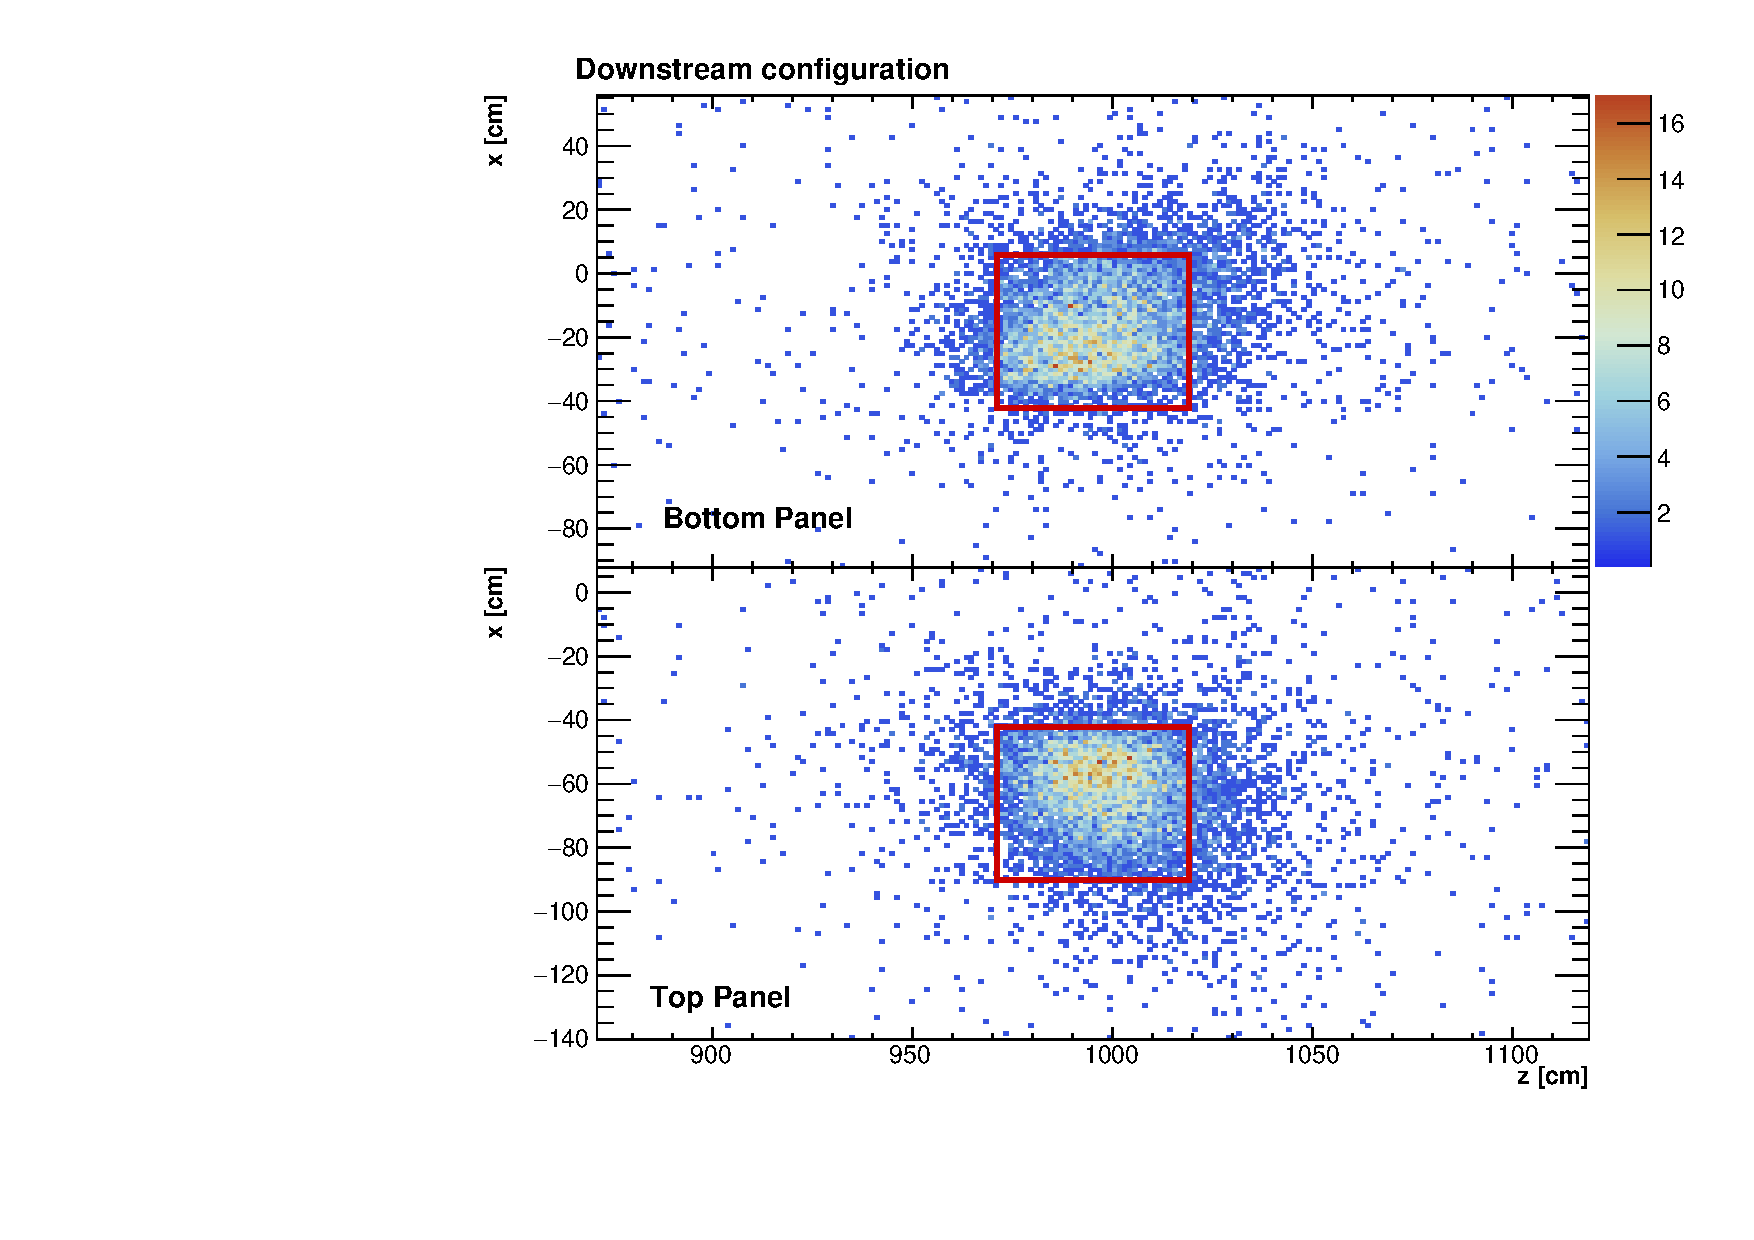
\includegraphics[width=\linewidth]{figures/downstream.pdf}
    \caption{Downstream} \label{fig:downstream_align}
  \end{subfigure}

  \caption{Monte Carlo simulation of the possible MuCS trajectories the three different MuCS setups used in this analysis. Brown tracks correspond to cosmic rays hitting both panels and the TPC, while red tracks go through the MuCS but miss the TPC.} \label{fig:alignment}
\end{figure}

The angular distribution of the MuCS-triggering cosmic rays, obtained extrapolating a line from the MuCS hits, has also been measured and compared with an independent Monte Carlo simulation, used only to check that the angular distribution of the cosmic rays was the same.  In this case, the Monte Carlo samples have been obtained generating a sample of cosmic rays within the top box borders. Each event is stored only if the cosmic ray crosses also the bottom box. This Monte Carlo information must not be confused with the reconstructed Monte Carlo information described above, which is obtained reconstructing a simulated cosmic ray in the TPC. Fig. \ref{fig:mucs_angles} shows that the distributions of the spherical angles have a good data/Monte Carlo agreement.

\begin{figure}[htbp]
  \begin{subfigure}{0.52\textwidth}
    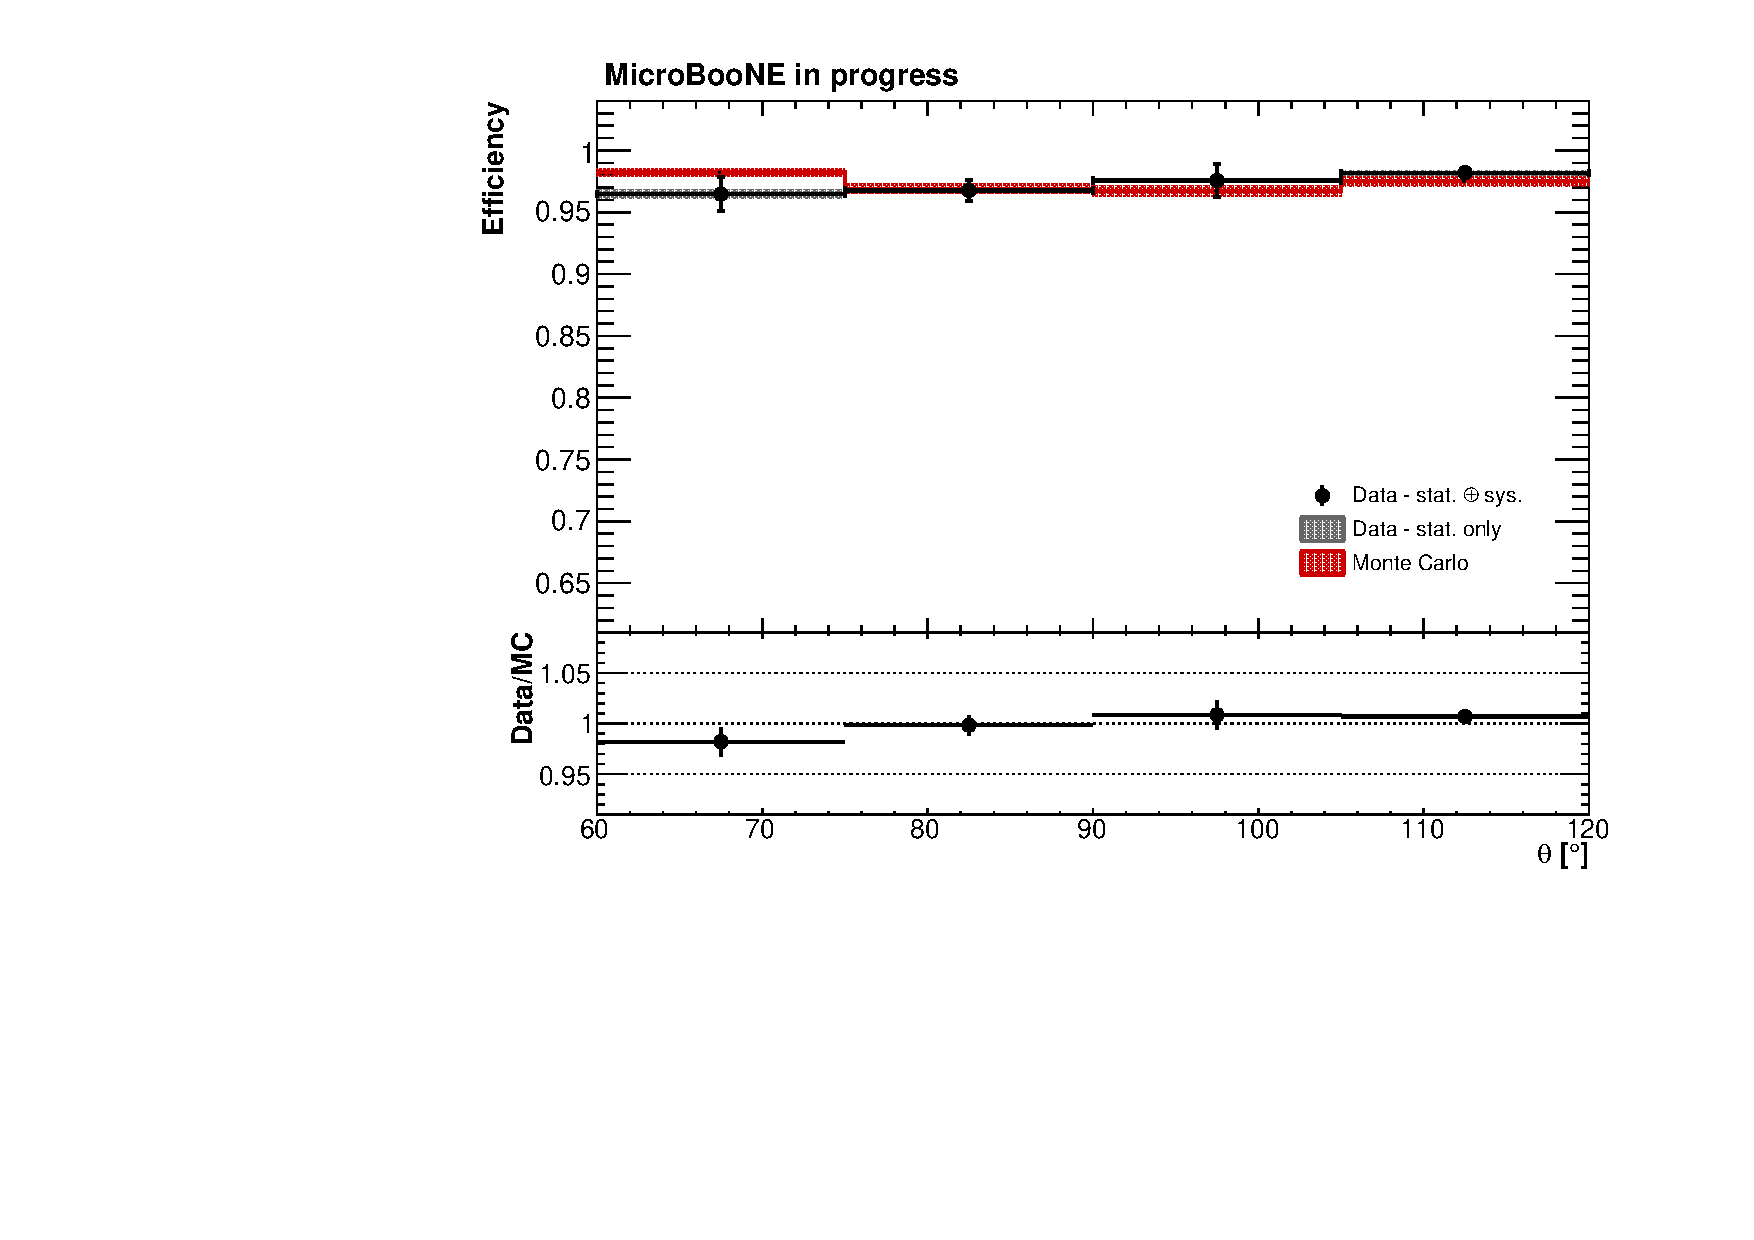
\includegraphics[width=\linewidth]{figures/theta.pdf}
    \caption{$\theta$ Data/Monte Carlo distribution.} \label{fig:xy_mucs}
  \end{subfigure}
  \begin{subfigure}{0.52\textwidth}
    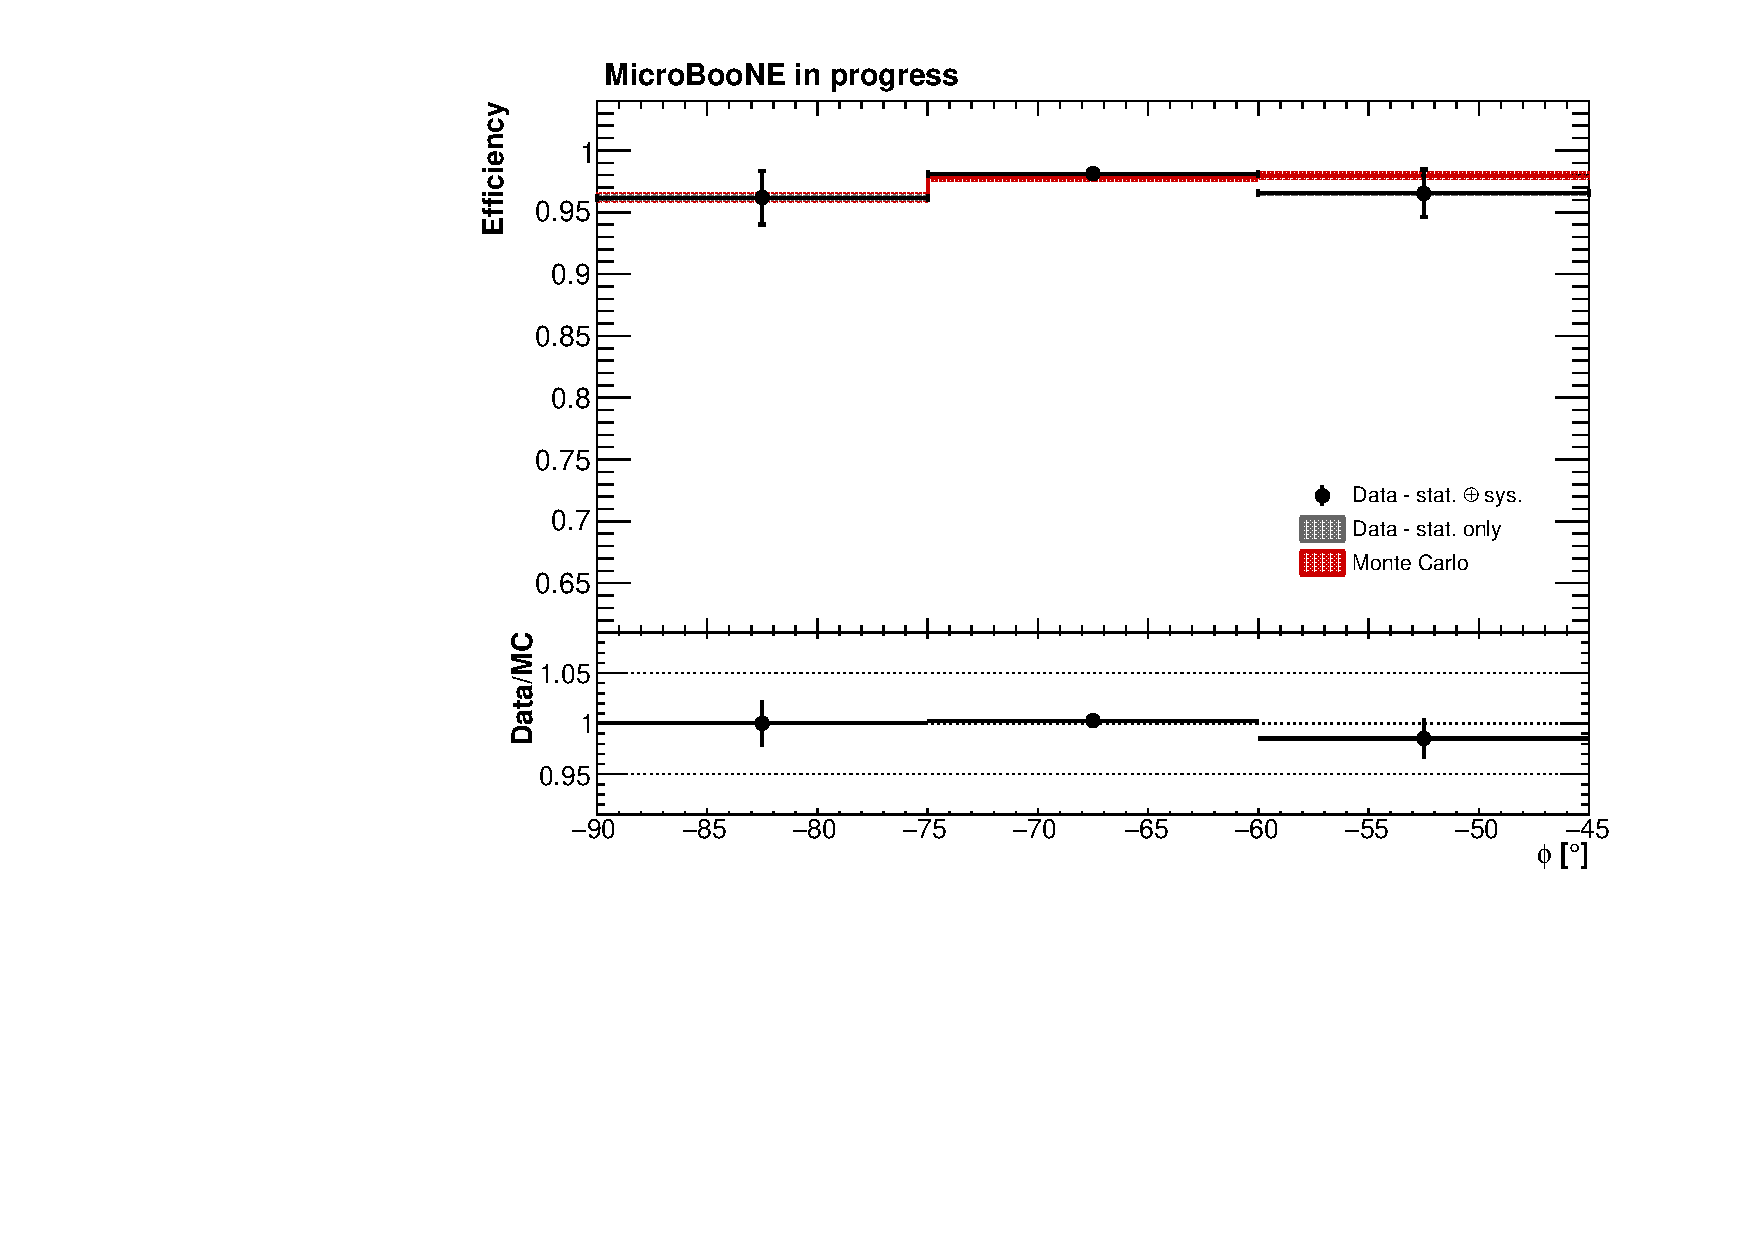
\includegraphics[width=\linewidth]{figures/phi.pdf}
    \caption{$\phi$ Data/Monte Carlo distribution.} \label{fig:yzmucs}
  \end{subfigure}
  \caption{Data/Monte Carlo distributions of the spherical angles of the cosmic rays hitting the MuCS. Data angles have been obtained extrapolating the MuCS hits. Errors are statistical only.} \label{fig:mucs_angles}


\end{figure}


\section{Reconstruction efficiencies}\label{sec:reco}
We define the data reconstruction efficiency $\epsilon$ as the ratio between the number events with a MuCS-reconstructed track and the number of MuCS-triggered events:
\begin{equation}
  \epsilon = \frac{\mathrm{N.~of~MuCS-reconstructed~events}}{\mathrm{N.~of~MuCS-triggered~events}}.
\end{equation}

However, the number of events with a MuCS-reconstructed track depends on the cut on the minimum distance between the MuCS-extrapolated track and the closest reconstructed track. Choosing a value too large, in fact, would overestimate our reconstruction efficiency. In this way, we would select events that do not have a reconstructed MuCS cosmic ray, but they happen to have another cosmic ray whose starting point is close to the extrapolated MuCS track.

On the other hand, with a tolerance too small we would underestimate the data reconstruction efficiency, since we would not count the events with a MuCS cosmic ray scattered more than the tolerance.

In order to choose the optimal value of the tolerance, we generated a MuCS Monte Carlo simulation for each geometrical configuration. Each Monte Carlo event will have a cosmic ray going through both MuCS panels, overlaid with a standard cosmic-ray event. The Monte Carlo dataset allows us to have a one-to-one association between a reconstructed track and a generated cosmic ray. It is then possible to measure the ideal reconstruction efficiency by comparing the number of MuCS cosmic rays with the number of events with a reconstructed MuCS cosmic ray. This value will not depend on the minimum distance and can be used as a reference: the optimal value of the tolerance is obtained when the measured reconstruction efficiency reaches the ideal reconstruction efficiency.

The purity of our sample will be defined as the ratio between the number of events with a real MuCS-reconstructed track within tolerance and the number of events with a reconstructed track within tolerance.

Fig. \ref{fig:purity} shows the purity and the reconstruction efficiency as a function of the tolerance. Their product (the ratio between real reconstructed MuCS tracks and MuCS-triggered events) will reach the ideal reconstruction efficiency at infinite and it is also shown. As we can see from the plot, the optimal value for the tolerance in our case is 32 cm, that corresponds to a purity of 98.9\%.

\begin{figure}[htbp]
  \begin{center}
    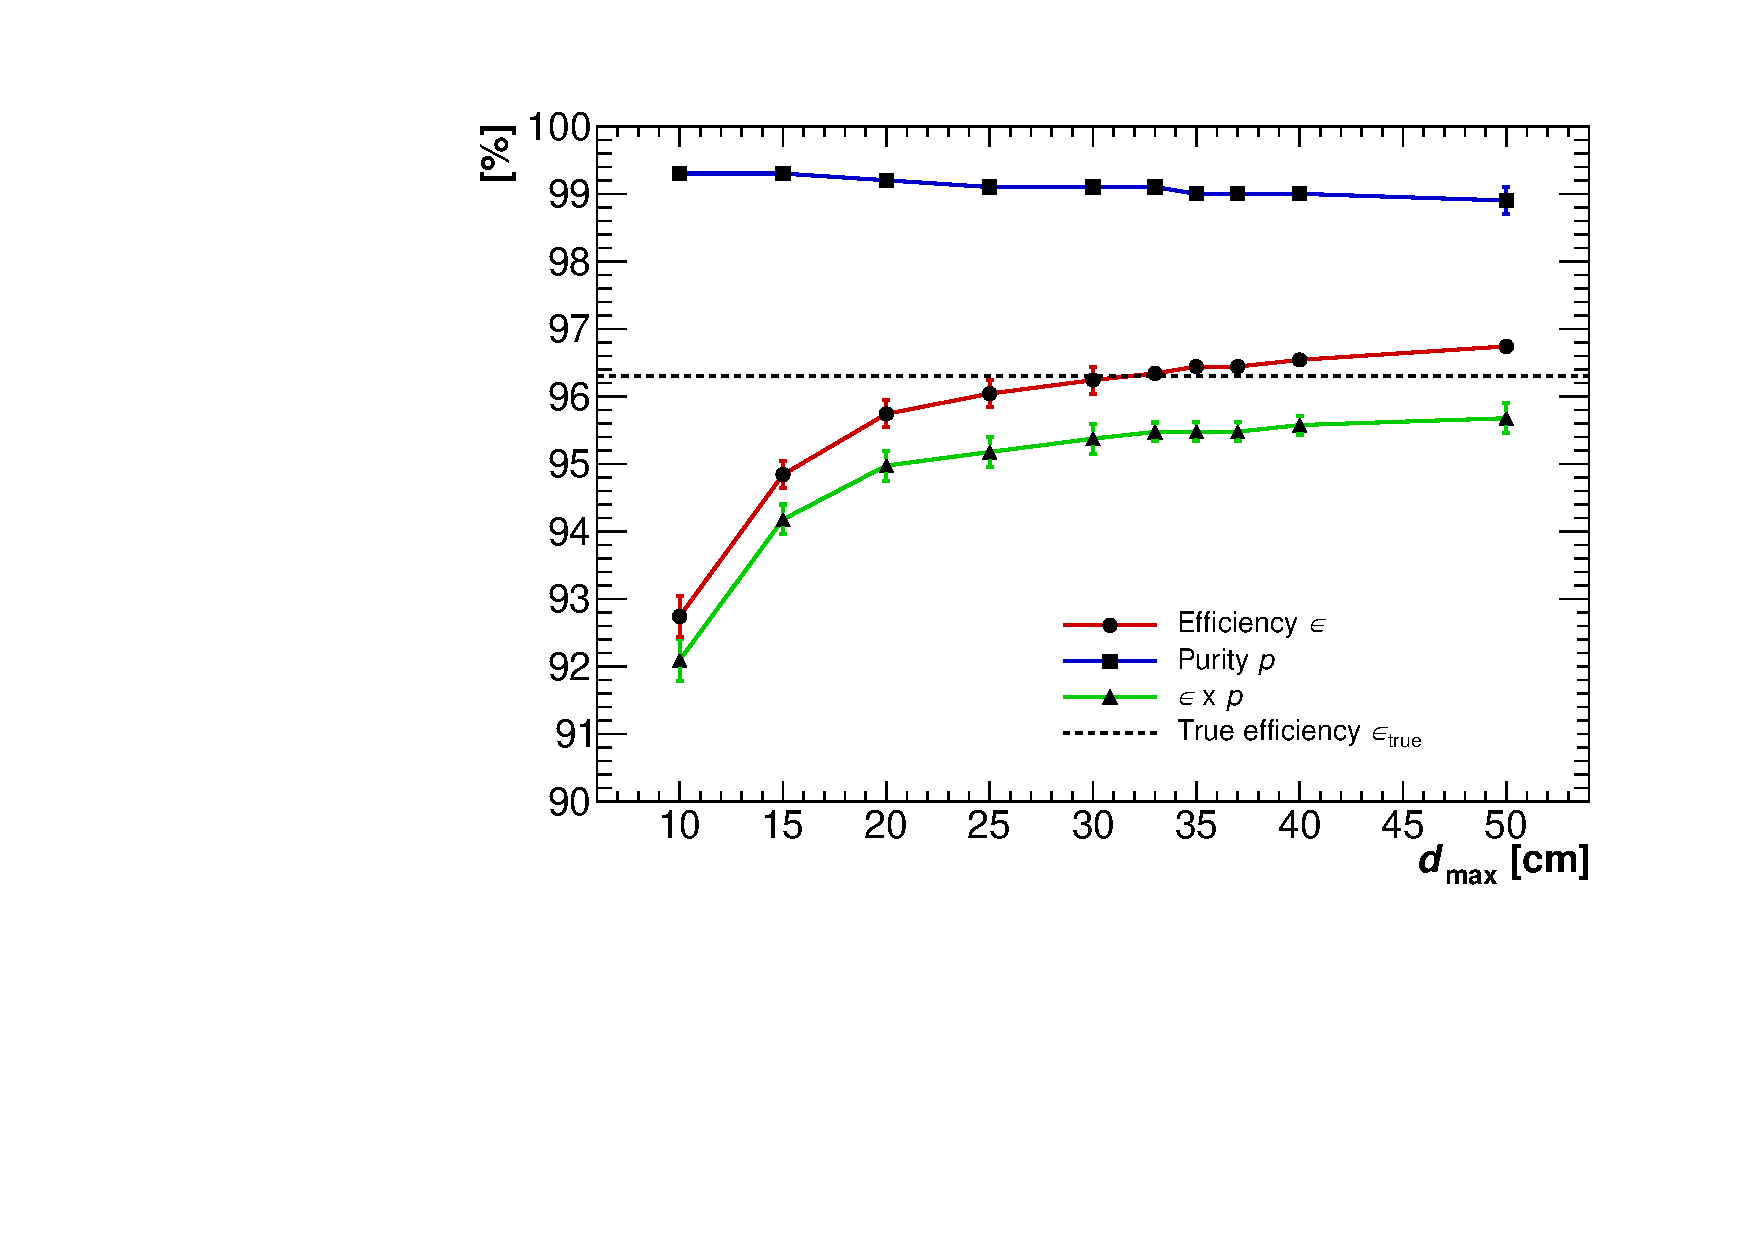
\includegraphics[width=0.7\linewidth]{figures/tolerance.pdf}
    \caption{Purity (blue), efficiency (red) and their product (green) as a function of the tolerance. The dashed line shows the ideal reconstruction efficiency.} \label{fig:purity}
  \end{center}
\end{figure}

Once we fixed the value of the minimum distance between a MuCS-extrapolated track and a reconstructed track, we can express the reconstruction efficiency as a function of the spherical starting angles $\theta$, $\phi$ and the expected track length in the TPC $L$, obtained from the MuCS hits. In an ideal TPC, in fact, the reconstruction efficiency for a MIP depends only on the number of wires hit, which is given univocally by the direction and the length of the track in the TPC.

Our efficiency can then be plotted as a three-dimensional histogram: each bin will correspond to a particular combination of the $\theta$, $\phi$, $L$ variables. Fig. \ref{fig:3d} shows both the data and the Monte Carlo reconstruction efficiency, generated as described in Sec. \ref{sec:merging}.

\begin{figure}[htbp]
  \begin{subfigure}{0.52\textwidth}
    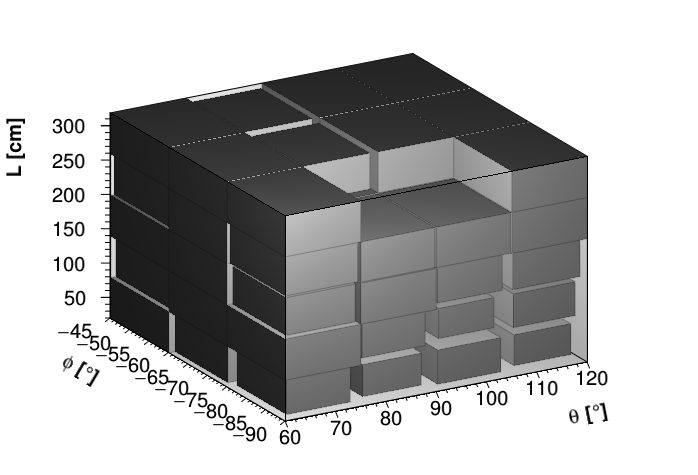
\includegraphics[width=\linewidth]{figures/3d_mc.png}
    \caption{Monte Carlo} \label{fig:3d_mc}
  \end{subfigure}
  \begin{subfigure}{0.52\textwidth}
    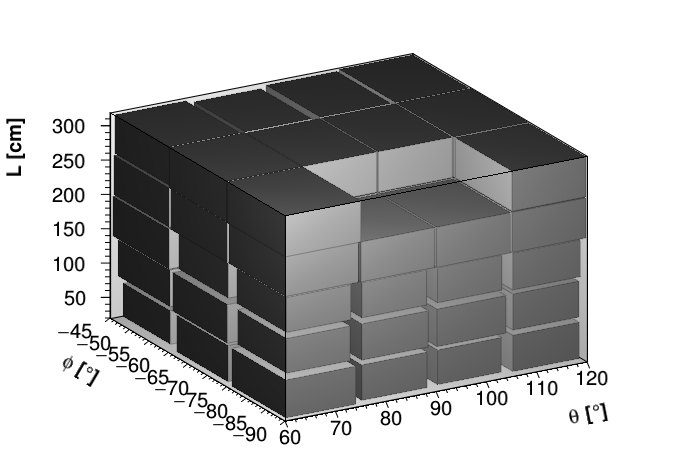
\includegraphics[width=\linewidth]{figures/3d_data.png}
    \caption{Data} \label{fig:3d_data}
  \end{subfigure}
  \caption{Monte Carlo and data three-dimensional reconstruction efficiency as a function of the starting angles $\theta$, $\phi$ and the extrapolated track length $L$.}
\end{figure}

\subsection{Detector non-uniformities}
The presence of detector non-uniformities can introduce a systematic error in the measurement of the reconstruction efficiency. In particular, the presence of missing wires in specific regions of the detector can lower the reconstruction efficiency in only one of our three dataset, since they cover different regions of the TPC.

To check if these non-uniformities introduce a systematic effect we measured the significance $\sigma$ of the difference between the efficiency measured in two different configurations:
\begin{equation}
\sigma = \frac{\epsilon_a-\epsilon_b}{\sqrt{\Delta \epsilon_{a}^2 + \Delta \epsilon_b^2}},
\end{equation}
where $\epsilon_{a}$ ($\epsilon_{b}$) is the reconstruction efficiency in the $a$ ($b$) configuration and $\Delta \epsilon_{a}$ ($\Delta \epsilon_{b}$) is its statistical error. This significance has been measured for each $\theta,\phi,L$ bin and for each possible combination of central, downstream and upstream configuration (described in Sec. \ref{sec:proc}). If there is a systematic effect, the standard deviation of the significances distribution should be larger than the unity. In our case, as shown in Fig. \ref{fig:significance}, the Gaussian fit of the distribution gives $\sigma = 1.54\pm0.12$, so significantly larger than 1.

\begin{figure}[htbp]
  \begin{center}
    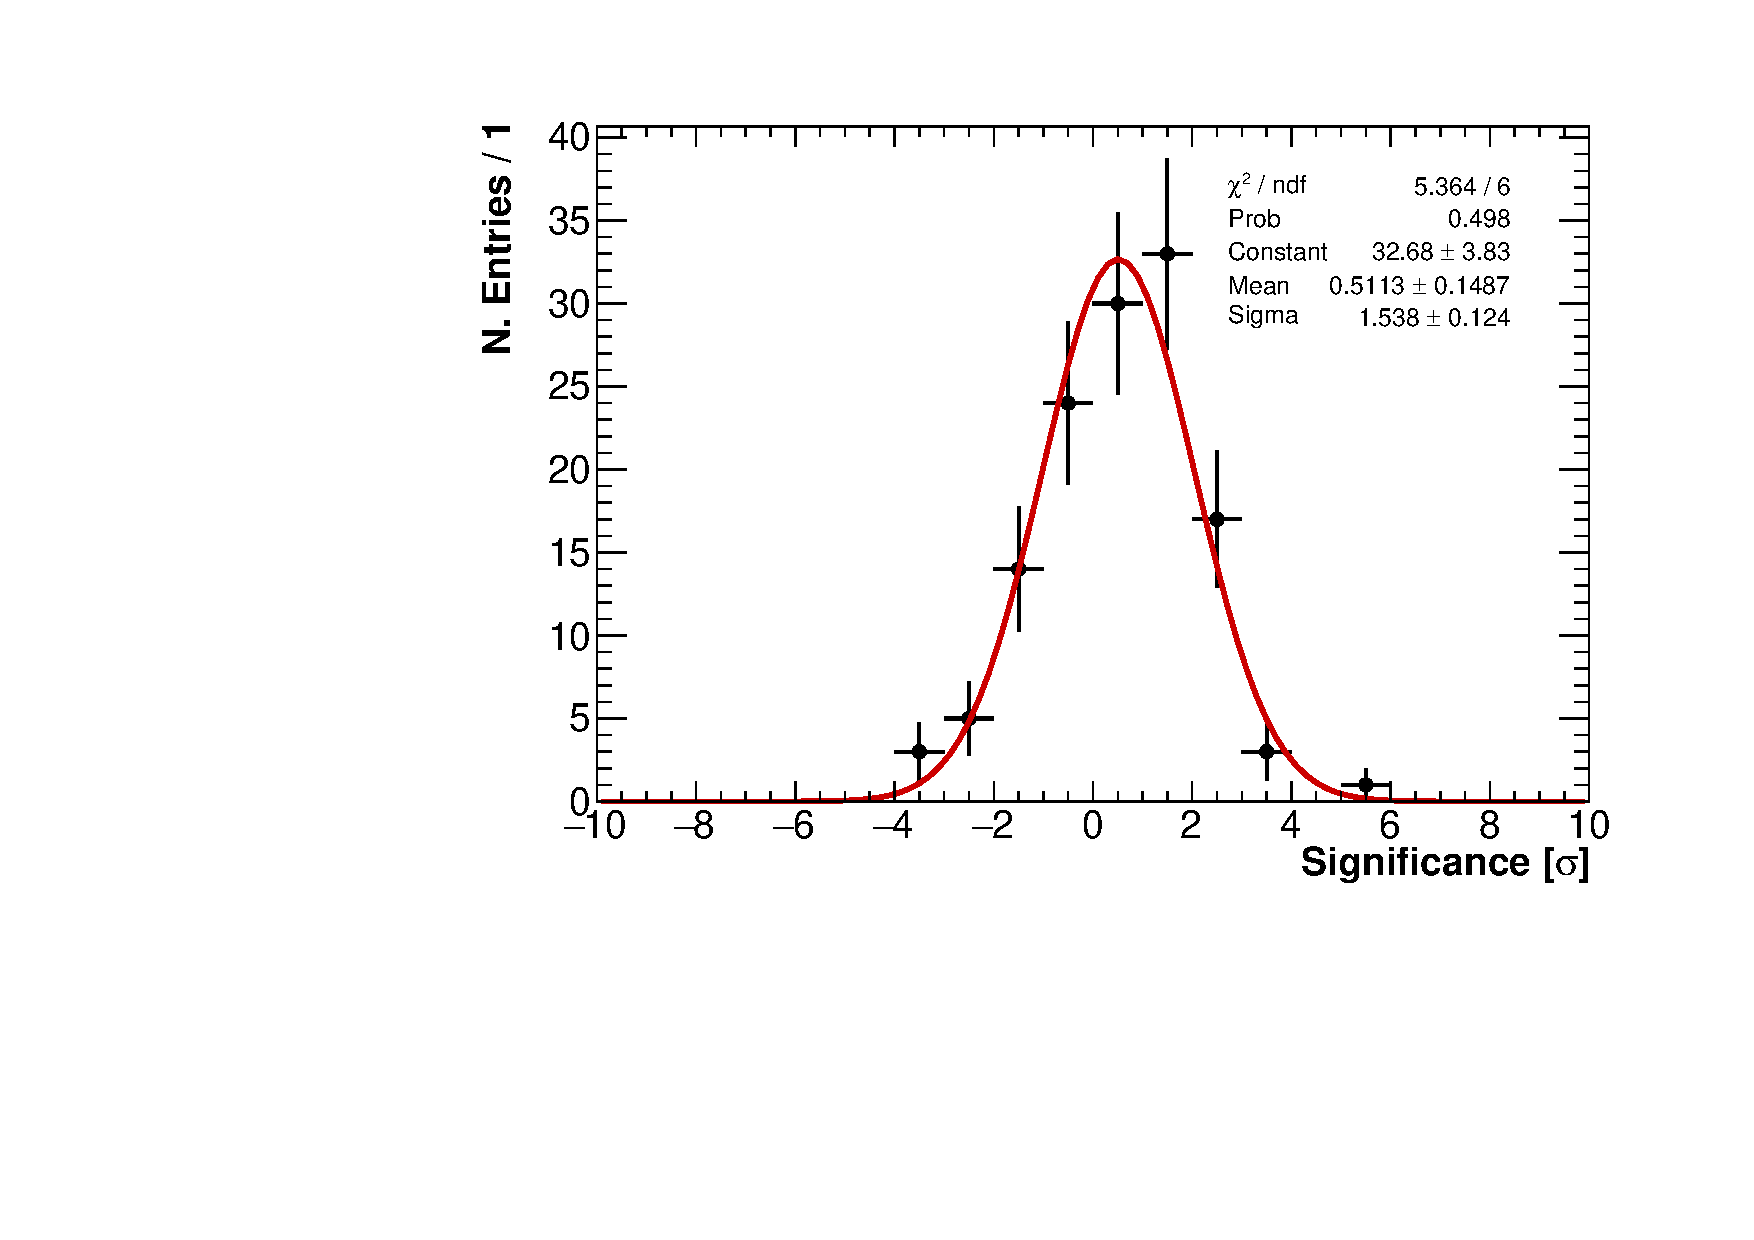
\includegraphics[width=0.7\linewidth]{figures/significance.pdf}
    \caption{Distribution of the significances of the reconstruction efficiency for each $\theta,\phi,L$ bin, measured for any combination of the three MuCS configuration.} \label{fig:significance}
  \end{center}
\end{figure}

In order to understand if these discrepancies are caused by missing wires in specific parts of detector, the bins corresponding to significances larger than 3 have been reported in Tab. \ref{tab:significance}.

\begin{table}[htbp]
  \centering
  \ra{1.2}
  \begin{tabular}{cccccccccccc}
    \toprule
    $\theta\thinspace[^\circ]$ & $\phi\thinspace[^\circ]$ & $L\thinspace[\mathrm{cm}]$ & \phantom{a} & \multicolumn{2}{c}{Central} & \phantom{a} & \multicolumn{2}{c}{Upstream} & \phantom{a} & \multicolumn{2}{c}{Downstream}\\
     \cmidrule{5-6} \cmidrule{8-9} \cmidrule{11-12}
      &  &  & & avg. & err. & & avg. & err. & & avg. & err.   \\
    \midrule
    75 & -60 & 20 & & \textbf{0.85} & \textbf{0.04} & & \textbf{0.85} & \textbf{0.02} & & 0.95 & 0.02\\
    90 & -90 & 140 & & 0.97 & 0.03 & & \textbf{0.70} & \textbf{0.07} & & 0.93 & 0.04\\
    90 & -90 & 200 & & 0.99 & 0.01 & & \textbf{0.96} & \textbf{0.01} & & 0.99 & 0.01\\
    90 & -60 & 140 & & 0.98 & 0.01 & & \textbf{0.96} & \textbf{0.01} & & 0.99 & 0.01\\
    90 & -60 & 200 & & 0.99 & 0.01 & & \textbf{0.96} & \textbf{0.01} & & 0.89 & 0.01\\

    \bottomrule
  \end{tabular}
  \caption{Reconstruction efficiency for each geometrical configuration with a difference significance larger than 3. The lowest value is reported in bold.}\label{tab:significance}
\end{table}

As we can see, the configuration with the lowest reconstruction efficiency in this cases is always the upstream one. The drawing of the extrapolated tracks that have those specific $\theta,\phi,L$ coordinates shows that, for the upstream configuration, the corresponding cosmic rays go through regions with missing wires in one of the induction planes (Fig. \ref{fig:wires}). Moreover, since their $\theta$ coordinate is close to $90^\circ$, they are also aligned with the wires of the collection plane. Thus, these cosmic rays have few hits in two out of three planes and the algorithm is not able to reconstruct a track.

\begin{figure}[htbp]
  \begin{center}
    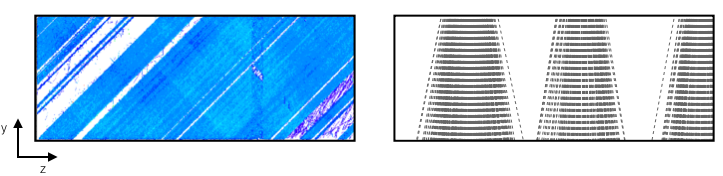
\includegraphics[width=1\linewidth]{figures/wire_tracks.png}
    \caption{Bi-dimensional plot of the average $dE/dx$, showing the region with missing wires on one of the induction planes (left) and extrapolated tracks corresponding to the coordinates in Tab. \ref{tab:significance} (right). As we can see, the tracks in the upstream part of the detector (low $z$) go through a region with several missing wires.} \label{fig:wires}
  \end{center}
\end{figure}




\begin{figure}[htbp]
  \begin{subfigure}{0.5\textwidth}
    \caption{3D data efficiency with \texttt{pandoraCosmic}.} \label{fig:pandora_3D}
  \end{subfigure}
  \hspace*{\fill}
  \begin{subfigure}{0.5\textwidth}
    \caption{3D Monte Carlo efficiency with \texttt{pandoraCosmic}.}\label{fig:pandora_3D_mc}
  \end{subfigure}
  \begin{subfigure}{0.5\textwidth}
    \caption{3D data efficiency with \texttt{pandoraCosmicKHit}.} \label{fig:pandoraKHit_3D}
  \end{subfigure}
  \hspace*{\fill}
  \begin{subfigure}{0.5\textwidth}
    \caption{3D Monte Carlo efficiency with \texttt{pandoraCosmicKHit}.}\label{fig:pandoraKHit_3D_mc}
  \end{subfigure}
  \begin{subfigure}{0.5\textwidth}
    \caption{3D data efficiency with \texttt{trackkalmanhit}.} \label{fig:tk_3D}
  \end{subfigure}
  \hspace*{\fill}
  \begin{subfigure}{0.5\textwidth}
    \caption{3D Monte Carlo efficiency with \texttt{trackkalmanhit}.}\label{fig:tk_3D_mc}
  \end{subfigure}
  \caption{Data (left) and Monte Carlo (right) 3D efficiencies  as a function of $\theta_{xy}$, $\theta_{yz}$ and $L$ for \texttt{track\-kal\-man\-hit}, \texttt{pan\-do\-ra\-Co\-smic} and \texttt{pan\-do\-ra\-Co\-smicKHit} reconstruction algorithms. Each box correspond to a particular combination of $\theta_{xy}, \theta_{yz}$ and $L$. Larger boxes correspond to larger efficiencies.} \label{fig:3Deff}
\end{figure}



\begin{figure}[htbp]
  \begin{subfigure}{0.52\textwidth}
    \caption{$\theta_{xy} - \theta_{yz}$, \texttt{pan\-do\-ra\-Co\-smic} - data} \label{fig:2d_pc1}
  \end{subfigure}
  \begin{subfigure}{0.52\textwidth}
    \caption{$\theta_{xy} - \theta_{yz}$, \texttt{pan\-do\-ra\-Co\-smic} - Monte Carlo}\label{fig:2d_pc1_mc}
  \end{subfigure}
  \begin{subfigure}{0.52\textwidth}
    \caption{$\theta_{xy} - L$, \texttt{pan\-do\-ra\-Co\-smic} - data}\label{fig:2d_pc2}
  \end{subfigure}
  \begin{subfigure}{0.52\textwidth}
    \caption{$\theta_{xy} - L$, \texttt{pan\-do\-ra\-Co\-smic} - Monte Carlo}\label{fig:2d_pc2_mc}
  \end{subfigure}
  \begin{subfigure}{0.52\textwidth}
    \caption{$\theta_{yz} - L$, \texttt{pan\-do\-ra\-Co\-smic} - data}\label{fig:2d_pc3}
  \end{subfigure}
  \begin{subfigure}{0.52\textwidth}
    \caption{$\theta_{yz} - L$, \texttt{pan\-do\-ra\-Co\-smic} - Monte Carlo}\label{fig:2d_pc3_mc}
  \end{subfigure}
  \caption{2D scatter-plot of the reconstruction efficiencies for data (left) and Monte Carlo (right) for $\theta_{xy} - \theta_{yz}$, $\theta_{xy} - L$ and $\theta_{yz} - L$ 2D projections with the \texttt{pandoraCosmic} algorithm. Regions with lower data efficiency correspond to cosmic ray with a small path length in the TPC.} \label{fig:2deff_pandora}
\end{figure}

\begin{figure}[htbp]
  \begin{subfigure}{0.52\textwidth}
    \caption{$\theta_{xy} - \theta_{yz}$, \texttt{pan\-do\-ra\-Co\-smicKHit} - data} \label{fig:2d_pk1}
  \end{subfigure}
  \begin{subfigure}{0.52\textwidth}
    \caption{$\theta_{xy} - \theta_{yz}$, \texttt{pan\-do\-ra\-Co\-smicKHit} - Monte Carlo}\label{fig:2d_pk1_mc}
  \end{subfigure}
  \begin{subfigure}{0.52\textwidth}
    \caption{$\theta_{xy} - L$, \texttt{pan\-do\-ra\-Co\-smicKHit} - data}\label{fig:2d_pk2}
  \end{subfigure}
  \begin{subfigure}{0.52\textwidth}
    \caption{$\theta_{xy} - L$, \texttt{pan\-do\-ra\-Co\-smicKHit} - Monte Carlo}\label{fig:2d_pk2_mc}
  \end{subfigure}
  \begin{subfigure}{0.52\textwidth}
    \caption{$\theta_{yz} - L$, \texttt{pan\-do\-ra\-Co\-smicKHit} - data}\label{fig:2d_pk3}
  \end{subfigure}
  \begin{subfigure}{0.52\textwidth}
    \caption{$\theta_{yz} - L$, \texttt{pan\-do\-ra\-Co\-smicKHit} - Monte Carlo}\label{fig:2d_pk3_mc}
  \end{subfigure}
  \caption{2D scatter-plot of the reconstruction efficiencies for data (left) and Monte Carlo (right) for $\theta_{xy} - \theta_{yz}$, $\theta_{xy} - L$ and $\theta_{yz} - L$ 2D projections with the \texttt{pandoraCosmicKHit} algorithm. Regions with lower data efficiency correspond to cosmic ray with a small path length in the TPC.} \label{fig:2deff_pandorak}
\end{figure}

\begin{figure}[htbp]
  \begin{subfigure}{0.52\textwidth}
    \caption{$\theta_{xy} - \theta_{yz}$, \texttt{trackkalmanhit} - data} \label{fig:2d_tk1}
  \end{subfigure}
  \begin{subfigure}{0.52\textwidth}
    \caption{$\theta_{xy} - \theta_{yz}$, \texttt{trackkalmanhit} - Monte Carlo}\label{fig:2d_tk1_mc}
  \end{subfigure}
  \begin{subfigure}{0.52\textwidth}
    \caption{$\theta_{xy} - L$, \texttt{trackkalmanhit} - data}\label{fig:2d_tk2}
  \end{subfigure}
  \begin{subfigure}{0.52\textwidth}
    \caption{$\theta_{xy} - L$, \texttt{trackkalmanhit} - Monte Carlo}\label{fig:2d_tk2_mc}
  \end{subfigure}
  \begin{subfigure}{0.52\textwidth}
    \caption{$\theta_{yz} - L$, \texttt{trackkalmanhit} - data}\label{fig:2d_tk3}
  \end{subfigure}
  \begin{subfigure}{0.52\textwidth}
    \caption{$\theta_{yz} - L$, \texttt{trackkalmanhit} - Monte Carlo}\label{fig:2d_tk3_mc}
  \end{subfigure}
  \caption{2D scatter-plot of the reconstruction efficiencies for data (left) and Monte Carlo (right) for $\theta_{xy} - \theta_{yz}$, $\theta_{xy} - L$ and $\theta_{yz} - L$ 2D projections with the \texttt{trackkalmanhit} algorithm. Regions with lower data efficiency correspond to cosmic ray with a small path length in the TPC. In general, this algorithm has lower data/Monte Carlo efficiencies w.r.t. to the ones using the Pandora framework.} \label{fig:2deff_trk}
\end{figure}

\begin{figure}[htbp]
  \begin{center}
    \begin{subfigure}{0.55\textwidth}
      \caption{Efficiency as a function of $\theta_{xy}$.} \label{fig:xy}
    \end{subfigure}\begin{subfigure}{0.55\textwidth}
    \caption{Efficiency as a function of $\theta_{yz}$}\label{fig:yz}
  \end{subfigure}
  \begin{subfigure}{0.55\textwidth}
    \caption{Efficiency as a function of $L$}\label{fig:l}
  \end{subfigure}
  \caption{Monte Carlo (boxes) and data (points) efficiencies  as a function of $\theta_{xy}$, $\theta_{yz}$ and $L$ for \texttt{track\-kal\-man\-hit} (red), \texttt{pan\-do\-ra\-Co\-smic} (blue) and \texttt{pan\-do\-ra\-Co\-smicKHit} (green) reconstruction algorithms. In general, data efficiency is always lower than the Monte Carlo one. In the case of the $L$ projection, the efficiency is proportional to the cosmic-ray path because a longer track has a larger number of hits in the TPC. The efficiency decreases when  $\theta_{xy}> -40^{\circ}$, because this angle corresponds to cosmic ray with a short path length.} \label{fig:eff}
\end{center}
\end{figure}

\begin{figure}[htbp]
  \begin{subfigure}{1\textwidth}
    \begin{center}

    \end{center}
    \caption{Short length of the cosmic ray.}\label{fig:short}
    \vspace{1em}
  \end{subfigure}
  \begin{subfigure}{1\textwidth}
    \begin{center}
      \caption{Missing wires in the expected region of the cosmic ray.}\label{fig:wire}
    \end{center}
  \end{subfigure}
  \caption{3D event reconstruction and corresponding event display for two MuCS-triggered events without tagged tracks. The red box (cross) in the 3D event corresponds to the data (Monte Carlo) flash. In the event on the top, the track was not reconstructed because the cosmic ray length in the TPC was too small. In the event on the bottom, the cosmic ray path was expected to be in a region with missing wires. The red boxes on the event display show the expected region for the cosmic ray tracks.} \label{fig:ineff}
\end{figure}
\clearpage{}


\section{CRY Monte Carlo dataset}\label{sec:cry}
From the study of the Monte Carlo dataset generated with 4 GeV (Sec. \ref{sec:reco}) and 500 MeV (Sec. \ref{sec:500mev}) fixed-energy cosmic rays it is possible to observe that the efficiency is energy-dependent. In particular, low-energy cosmic rays have a lower reconstruction efficiency, because of increased multiple Coulomb scattering.

Thus, in order to obtain a better Data/MC agreement we generated a new Monte Carlo sample using a complete cosmic-ray energy spectrum.

In this section, since our target is to obtain an efficiency-corrected cosmic-ray flux measurement, we will use the $\theta$ and $\phi$ angular coordinates, as defined in the MicroBooNE coordinate system \cite{datamc}:
\begin{equation}
  \begin{aligned}
    r &= \sqrt{x^2+y^2+z^2}\\
    \theta &= \mathrm{arccos}\frac{z}{r}\\
    \phi &= \arctan \frac{y}{x}.
  \end{aligned}
\end{equation}

In our procedure, we generate a complete CRY simulation with 1000 events (1 cosmic ray per event) for each bin of the $\theta$, $\phi$ parameter space, while the separation of the events on the $L$ axis is given automatically by the geometry. In order to account for the angular dependence of the cosmic-ray flux, each three-dimensional bin is normalized by the number of MuCS-triggered events in the same bin, given by the data (Sec. \ref{sec:flux}). In this way, it is possible to incorporate the effects of the energy dependence in the measurement of the Monte Carlo efficiency.

For each event, we check if there is a reconstructed track that, extrapolated up to the MuCS box heights, crosses both boxes, with the same procedure used for data and described in Sec. \ref{sec:proc}.
Since with this procedure we don't have a one-to-one correspondence between a MuCS-triggered event and a Monte Carlo event, the Monte Carlo efficiency is defined as:
\begin{equation}
  \epsilon(\theta,\phi,L) = \frac{\mathrm{N.~of~reco.~events}}{\mathrm{N.~of~generated~events}}.
\end{equation}
In order to remove stopping muon events, the same cut described in Sec. \ref{sec:mip} is applied to the generated events.

The 3D $\theta$-$\phi$-$L$ efficiency for data, Monte Carlo and data/Monte Carlo ratio, obtained with the \texttt{pandoraCosmic}, is shown in Fig. \ref{fig:cry_mc_3d}.
Figg. \ref{fig:cry_mc_2d}, \ref{fig:cry_mc_2d_2} and \ref{fig:cry_mc_2d_3} show the $\theta-\phi$, $\theta-L$ and $\phi-L$ 2D projections, respectively, while the 1D projections are shown in Fig. \ref{fig:cry_mc_1d}.

Tab. \ref{tab:mc} reports the overall efficiencies for data, fixed-energy Monte Carlo samples (4 GeV and 500 MeV) and CRY sample. As we can see, this procedure sensibly improves the data/Monte Carlo agreement: the overall efficiency for Monte Carlo is $(85.0\pm0.1)\%$, compared with the $(96.5\pm0.2)\%$ obtained with the 4 GeV fixed-energy sample.

\begin{table}[htbp]
  \centering
  \ra{1.2}
  \begin{tabular}{lcrrrcccccccc}
    \toprule
    & \phantom{a}& \multicolumn{2}{c}{Data} & \phantom{a} & \multicolumn{2}{c}{4 GeV MC} & \phantom{a} & \multicolumn{2}{c}{500 MeV MC} & \phantom{a} & \multicolumn{2}{c}{CRY MC}\\
    \cmidrule{3-4} \cmidrule{6-7} \cmidrule{9-10} \cmidrule{12-13}
    & & avg. & err. & & avg. & err. & & avg. & err. & & avg. & err.\\
    \midrule
    Efficiency & & 84.6 & 0.4 & & 96.5 & 0.2 & & 81.4 & 0.4 & & 85.0 & 0.1\\
    \bottomrule
  \end{tabular}
  \caption{Overall efficiencies for data, 4 GeV Monte Carlo, 500 MeV Monte Carlo and CRY Monte Carlo. Errors are statistical only.}\label{tab:mc}
\end{table}

\begin{figure}[htbp]
  \begin{center}
    \begin{subfigure}{0.52\textwidth}
      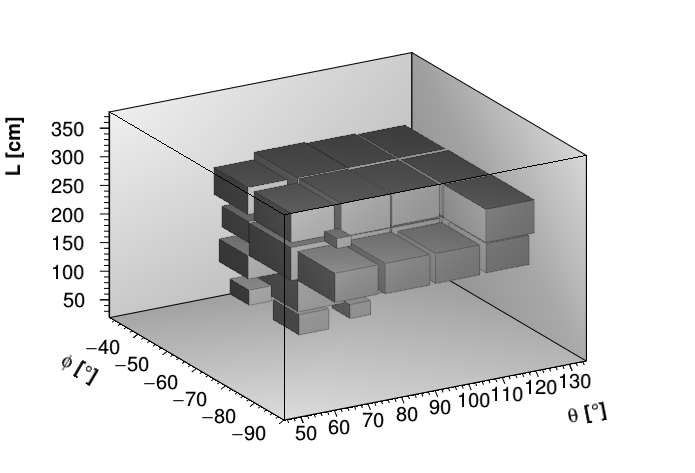
\includegraphics[width=\linewidth]{figures/theta_phi_l_data.png}
      \caption{$\theta - \phi - L$, data} \label{fig:3d_cry}
    \end{subfigure}\begin{subfigure}{0.52\textwidth}
    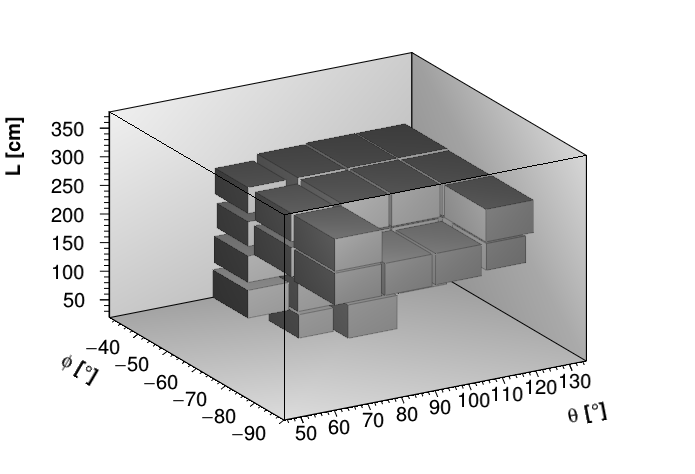
\includegraphics[width=\linewidth]{figures/theta_phi_l_mc.png}
    \caption{$\theta - \phi - L$, Monte Carlo}\label{fig:3d_cry_mc}
  \end{subfigure}
  \begin{subfigure}{0.52\textwidth}
    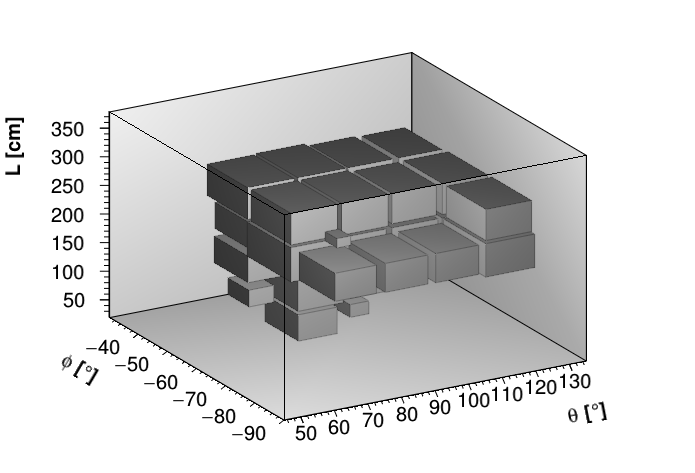
\includegraphics[width=\linewidth]{figures/ratio_theta_phi_l.png}
    \caption{$\theta - \phi - L$, data/Monte Carlo}\label{fig:3d_cry_ratio}
  \end{subfigure}
  \caption{3D $\theta - \phi - L$ efficiency with th \texttt{pandoraCosmic} algorithm for data, Monte Carlo and data/Monte Carlo ratio.} \label{fig:cry_mc_3d}
\end{center}
\end{figure}

\begin{figure}[htbp]
  \begin{center}
    \begin{subfigure}{0.52\textwidth}
      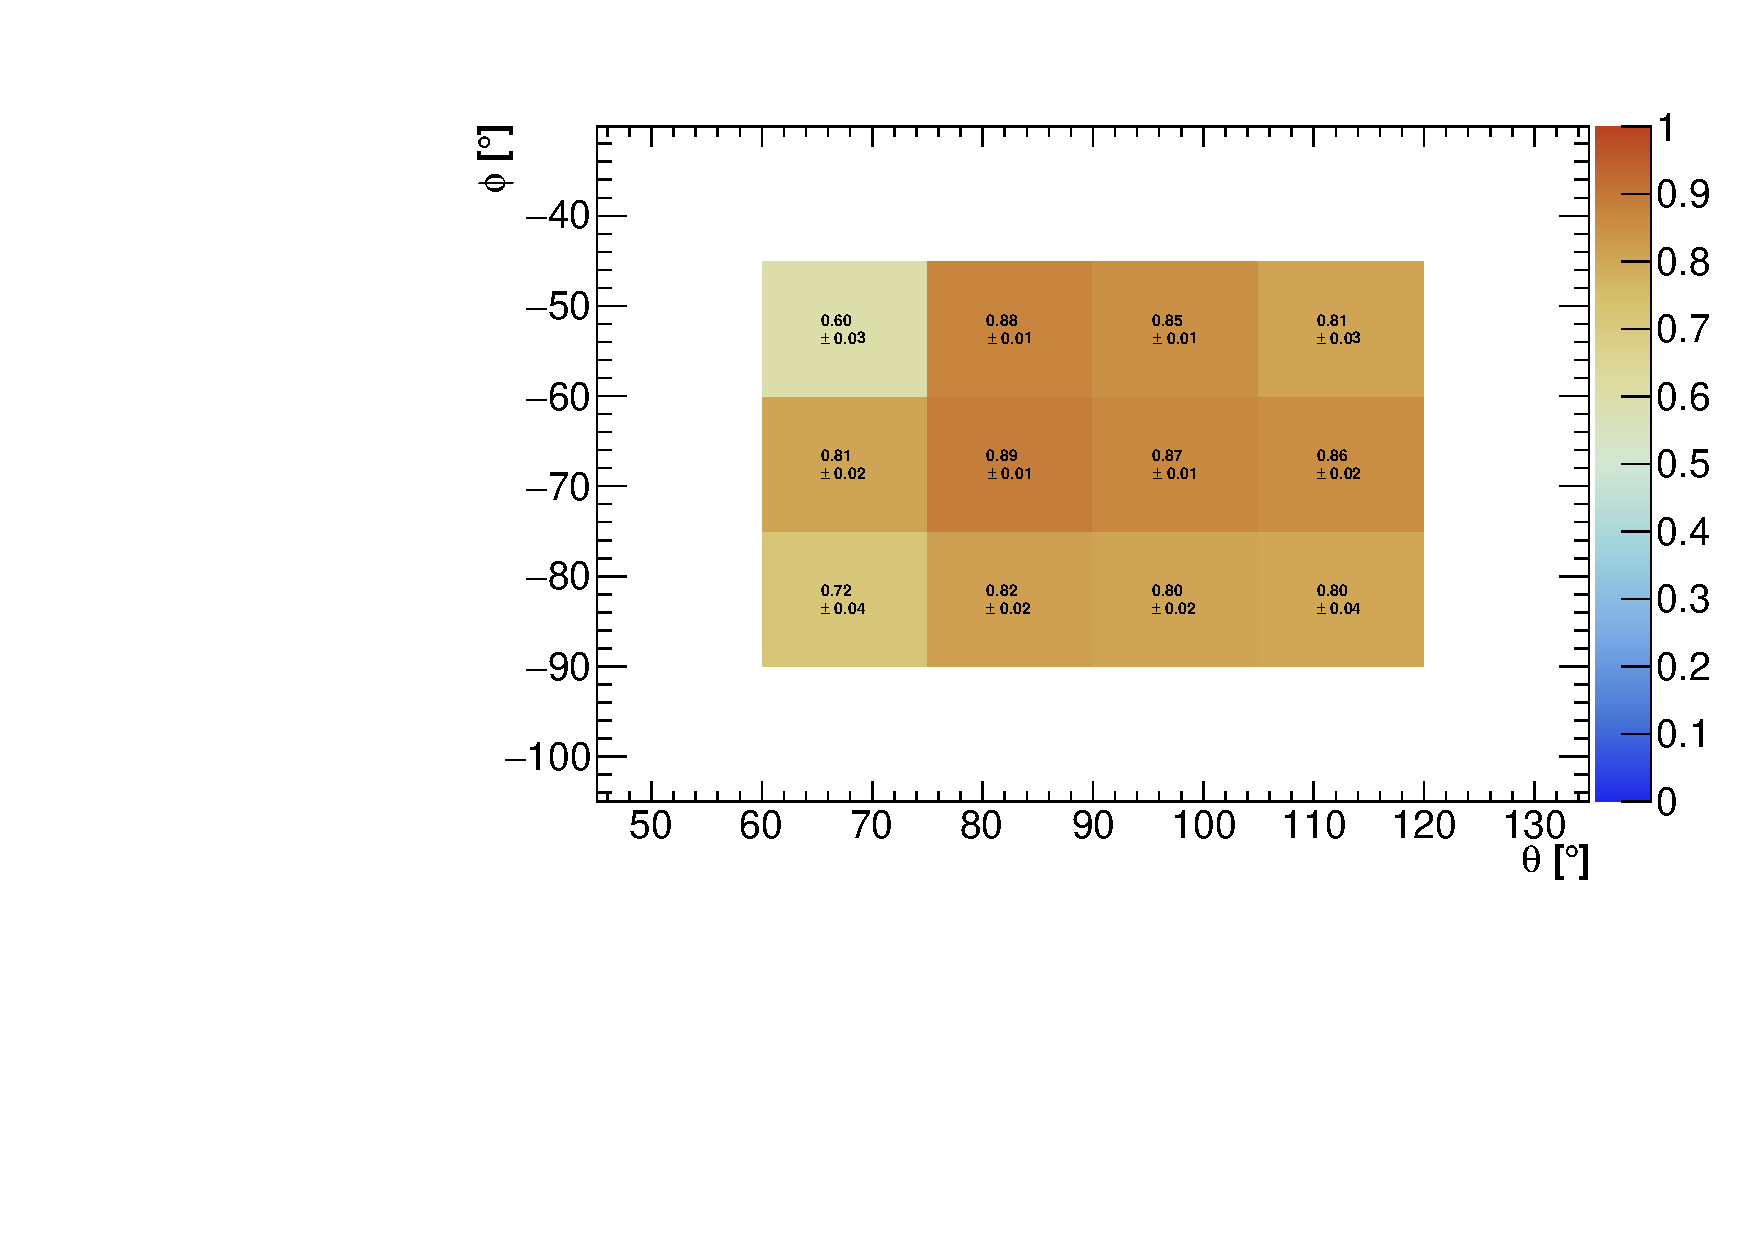
\includegraphics[width=\linewidth]{figures/theta_phi_data.pdf}
      \caption{$\theta - \phi$, data} \label{fig:2d_cry}
    \end{subfigure}\begin{subfigure}{0.52\textwidth}
    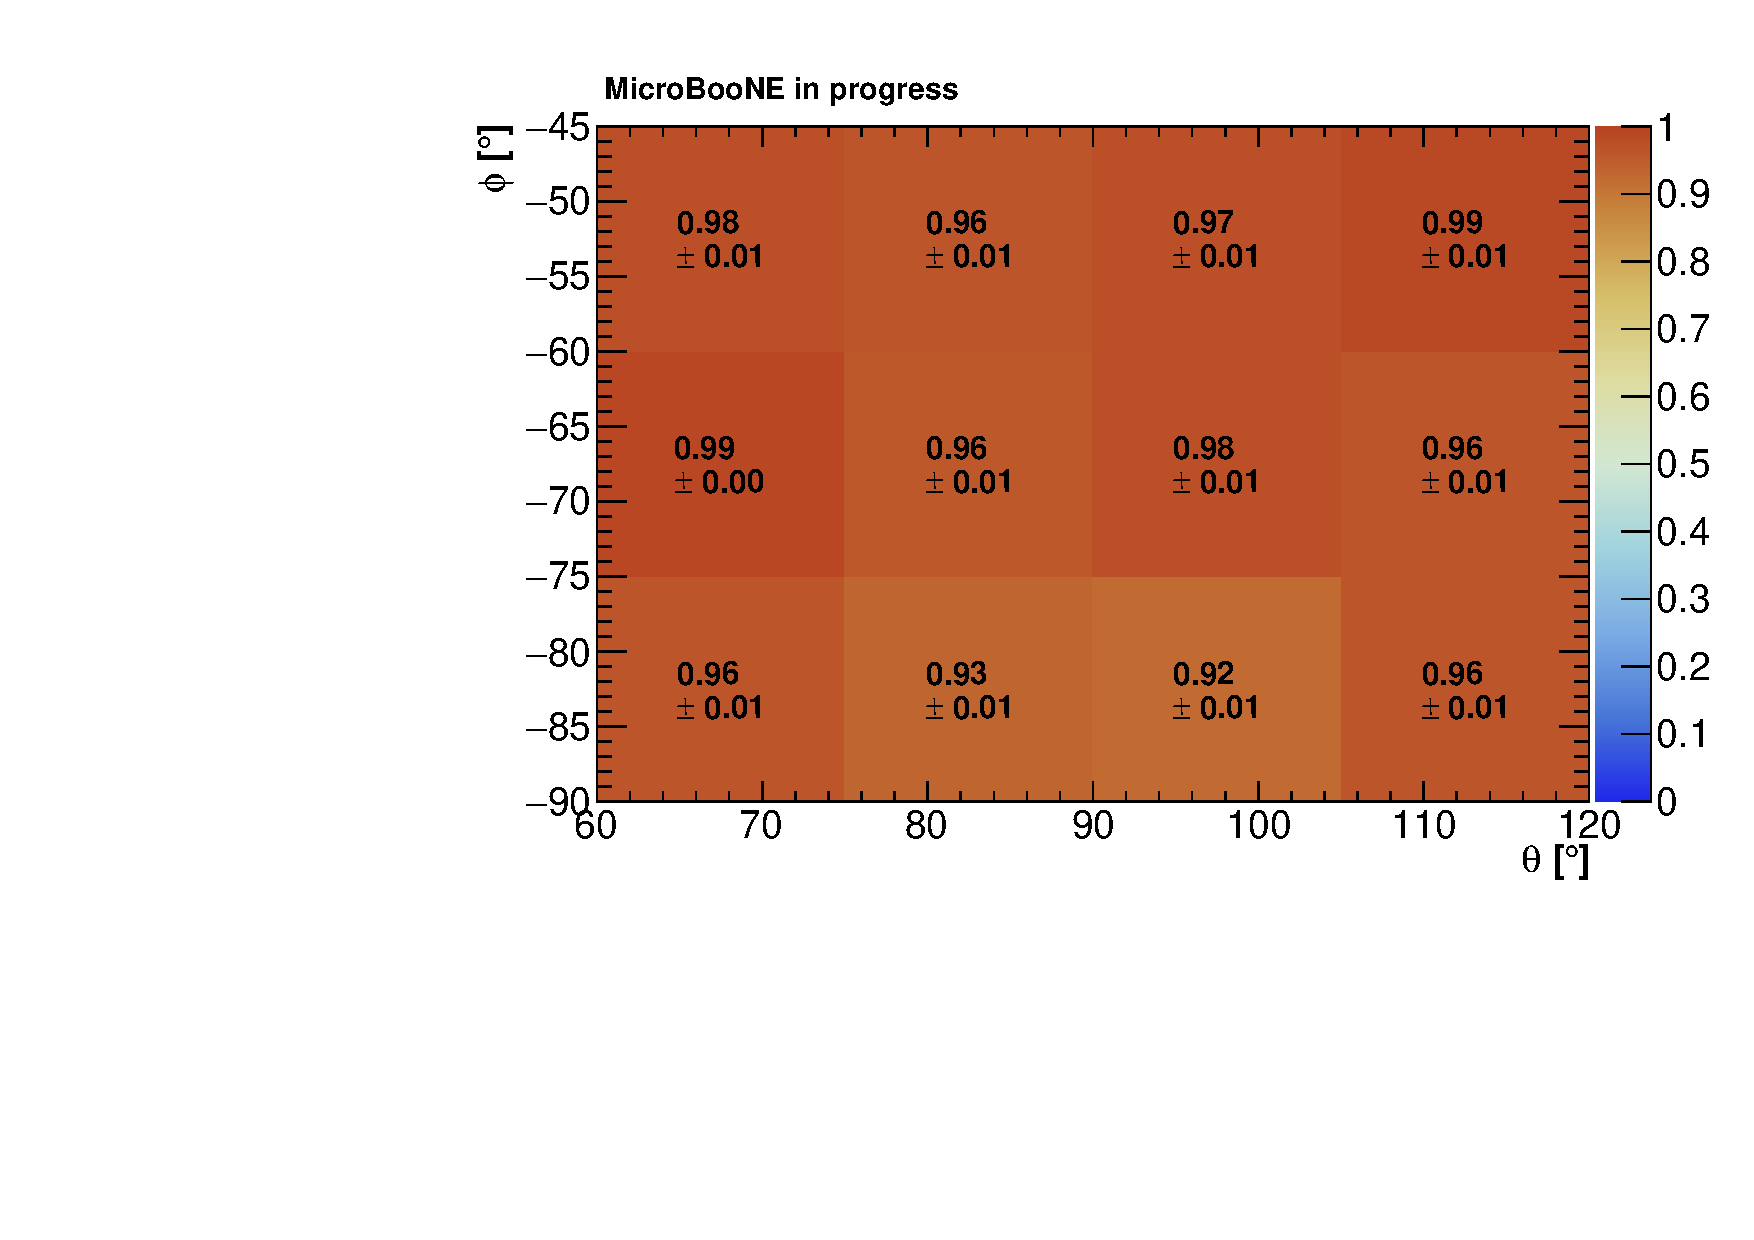
\includegraphics[width=\linewidth]{figures/theta_phi_mc.pdf}
    \caption{$\theta - \phi$, Monte Carlo}\label{fig:2d_cry_mc}
  \end{subfigure}
  \begin{subfigure}{0.52\textwidth}
    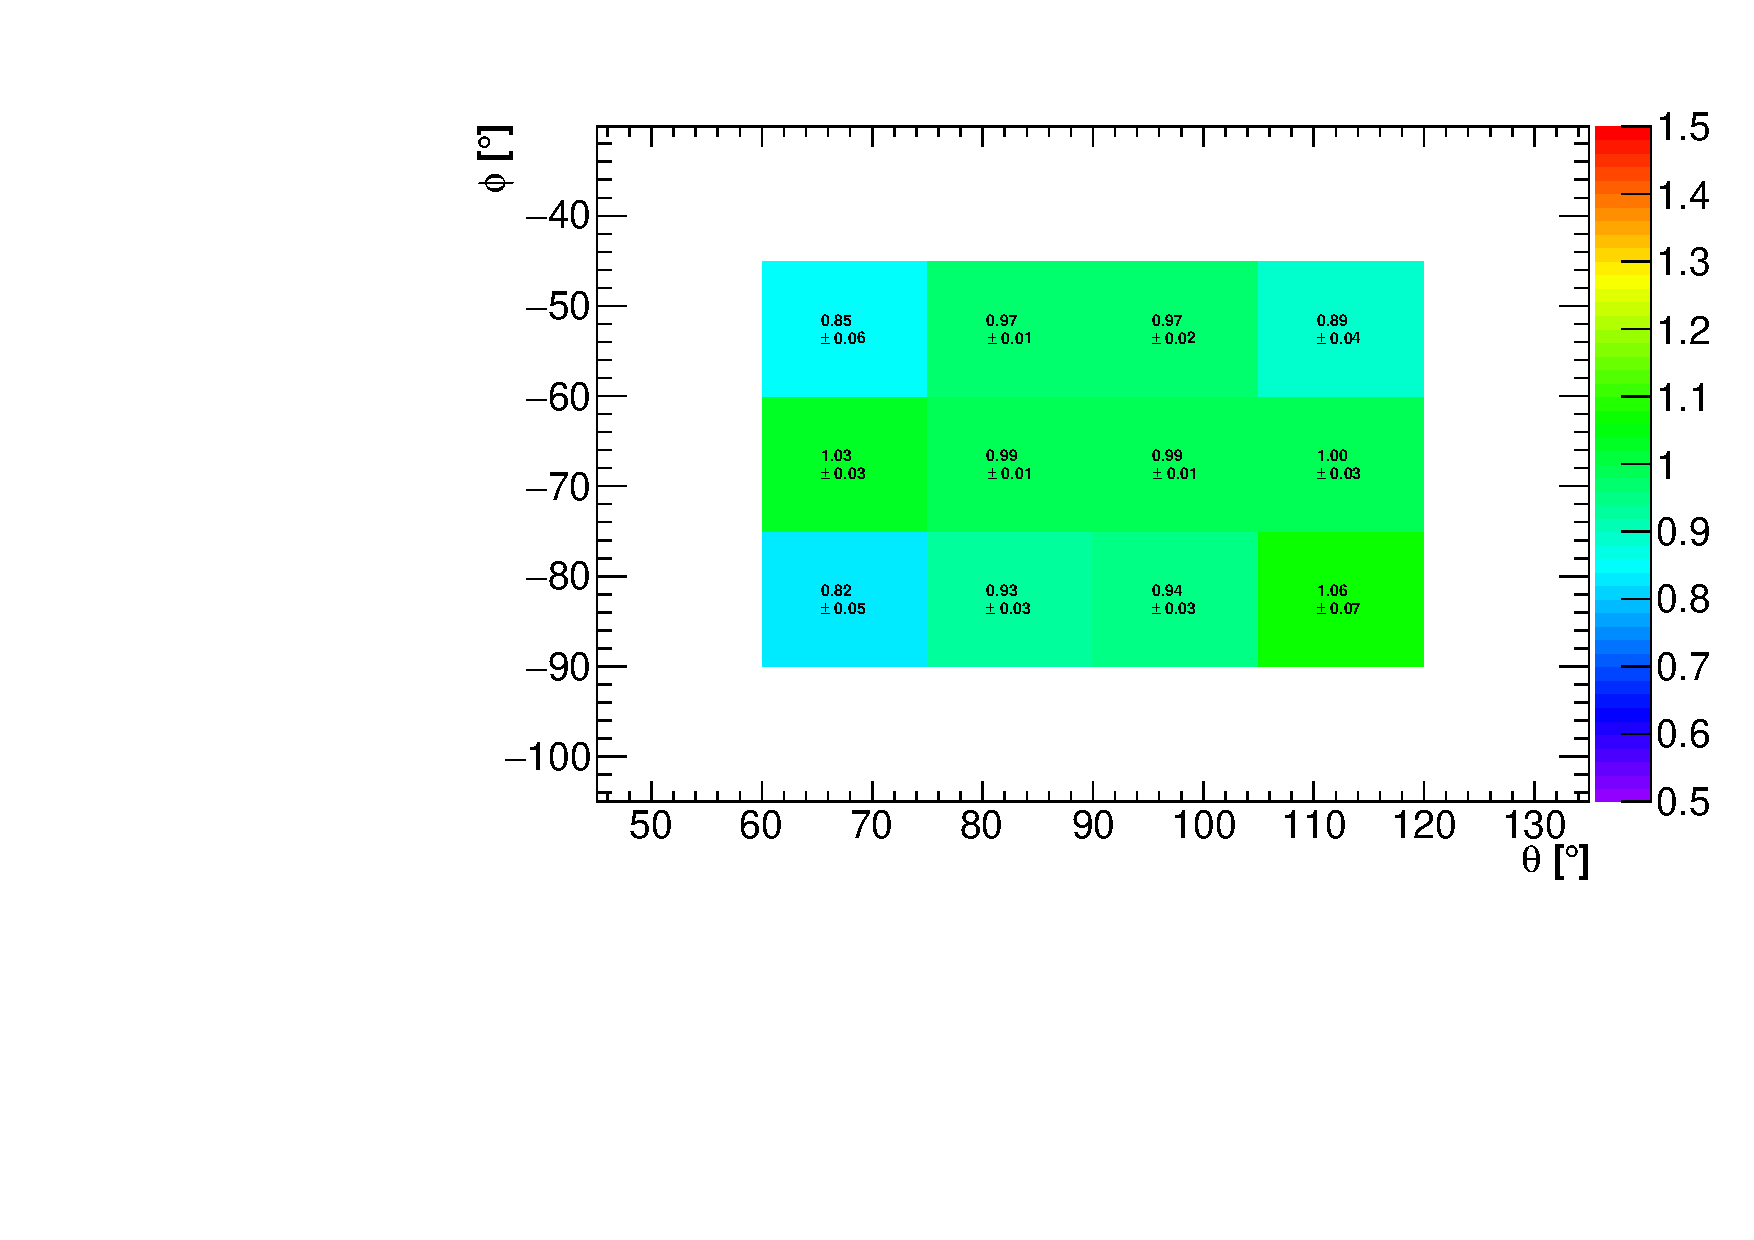
\includegraphics[width=\linewidth]{figures/ratio_theta_phi.pdf}
    \caption{$\theta - \phi$, data/Monte Carlo}\label{fig:2d_cry_ratio}
  \end{subfigure}
  \caption{2D $\theta - \phi$ efficiency with the \texttt{pandoraCosmic} algorithm for data, Monte Carlo and data/Monte Carlo ratio.} \label{fig:cry_mc_2d}
\end{center}
\end{figure}

\begin{figure}[htbp]
  \begin{center}
    \begin{subfigure}{0.52\textwidth}
      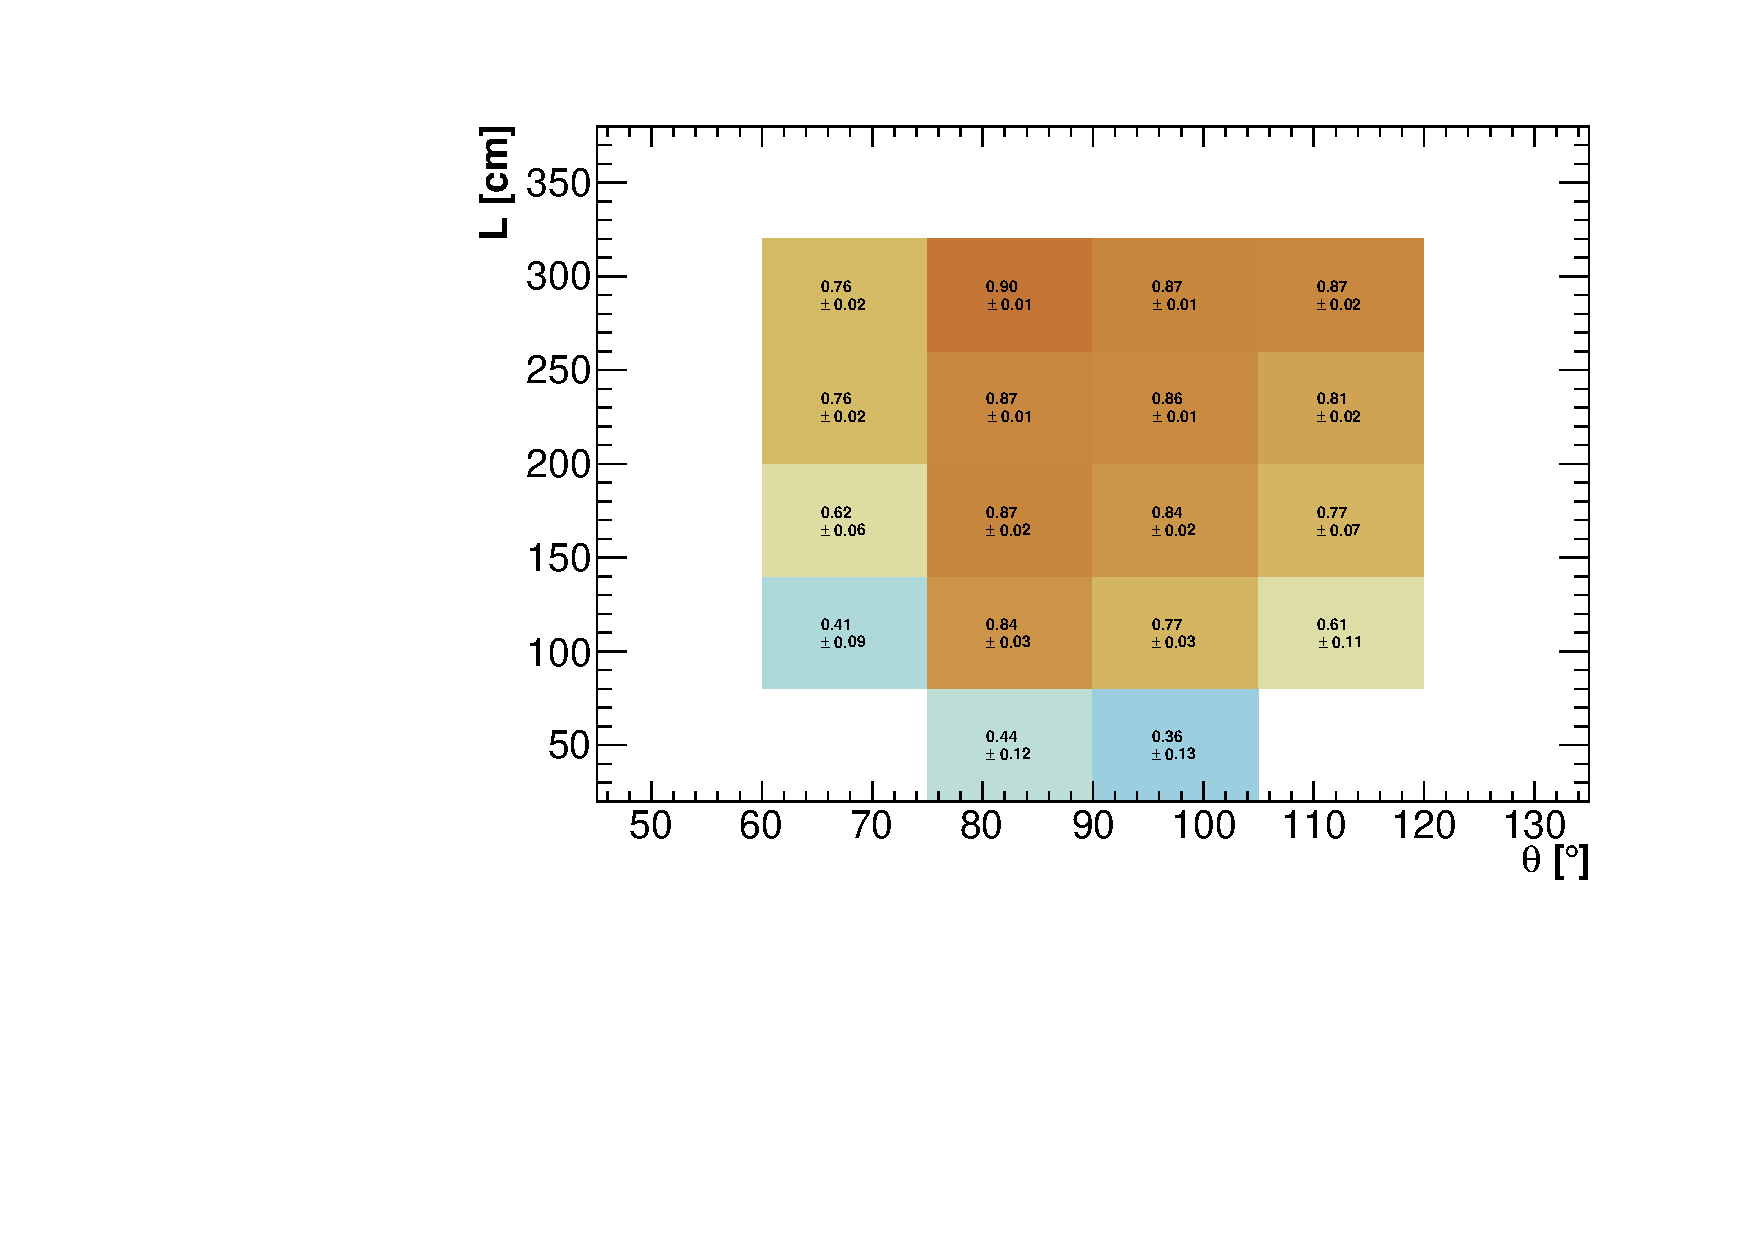
\includegraphics[width=\linewidth]{figures/theta_l_data.pdf}
      \caption{$\theta - L$, data} \label{fig:2d_cry_2}
    \end{subfigure}\begin{subfigure}{0.52\textwidth}
    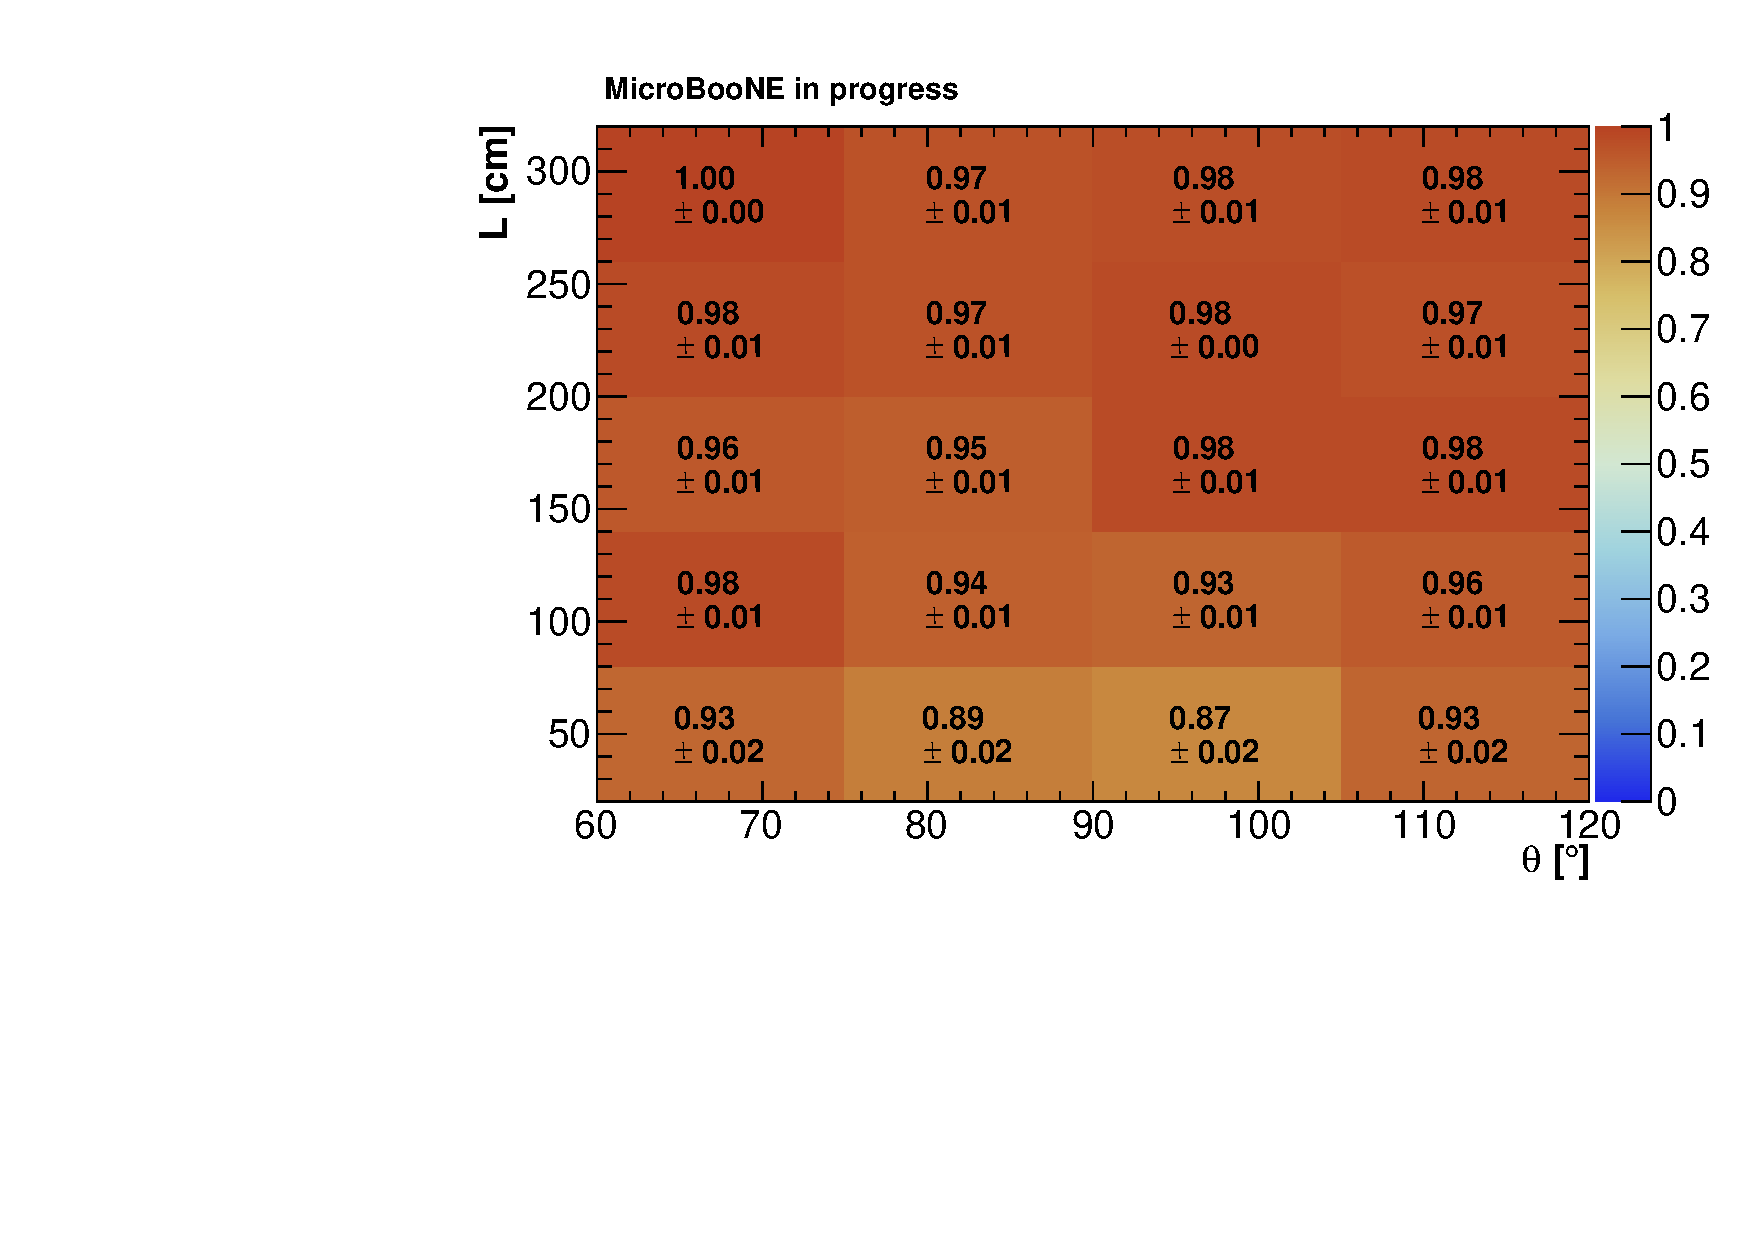
\includegraphics[width=\linewidth]{figures/theta_l_mc.pdf}
    \caption{$\theta - L$, Monte Carlo}\label{fig:2d_cry_mc_2}
  \end{subfigure}
  \begin{subfigure}{0.52\textwidth}
    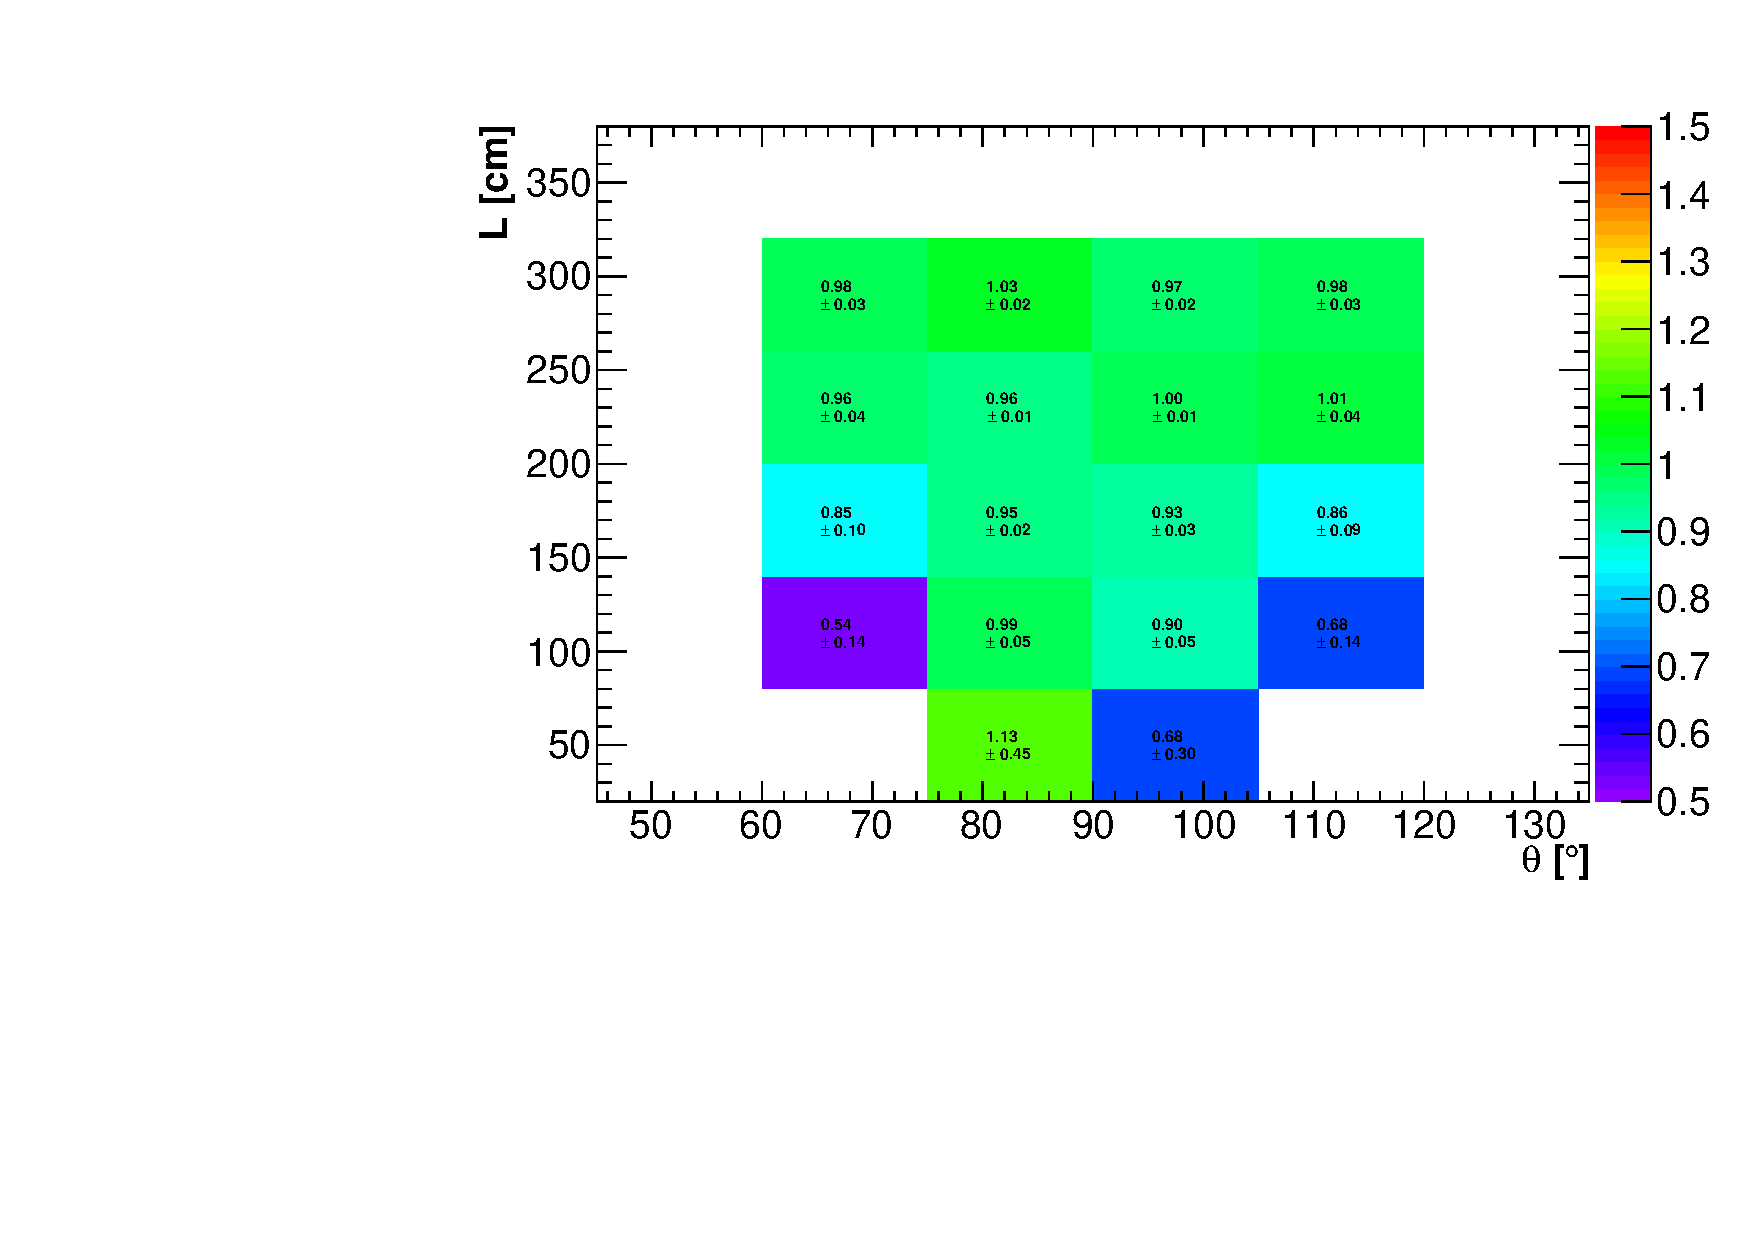
\includegraphics[width=\linewidth]{figures/ratio_theta_l.pdf}
    \caption{$\theta - L$, data/Monte Carlo}\label{fig:2d_cry_ratio_2}
  \end{subfigure}
  \caption{2D $\theta - L$ efficiency with the \texttt{pandoraCosmic} algorithm for data, Monte Carlo and data/Monte Carlo ratio.} \label{fig:cry_mc_2d_2}
\end{center}
\end{figure}

\begin{figure}[htbp]
  \begin{center}
    \begin{subfigure}{0.52\textwidth}
      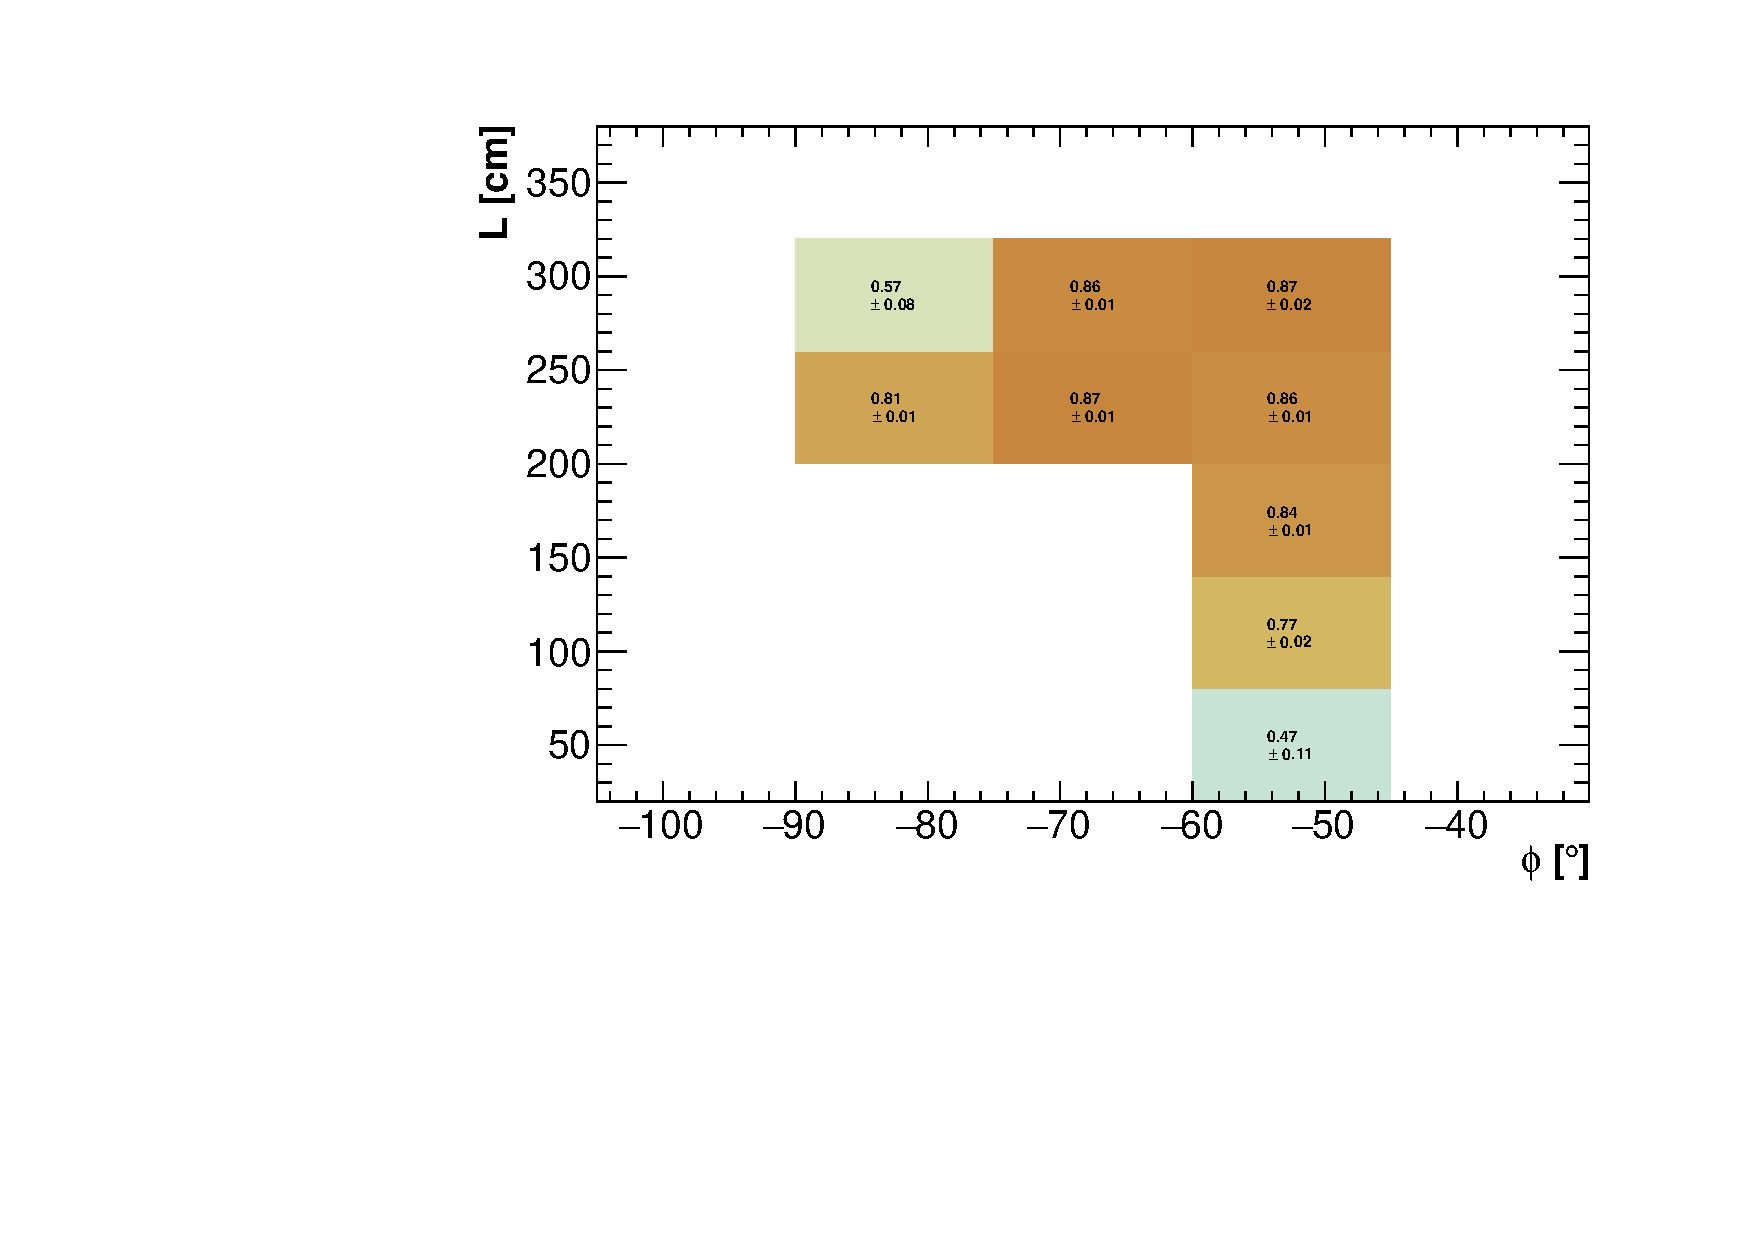
\includegraphics[width=\linewidth]{figures/phi_l_data.pdf}
      \caption{$\phi - L$, data} \label{fig:2d_cry_3}
    \end{subfigure}\begin{subfigure}{0.52\textwidth}
    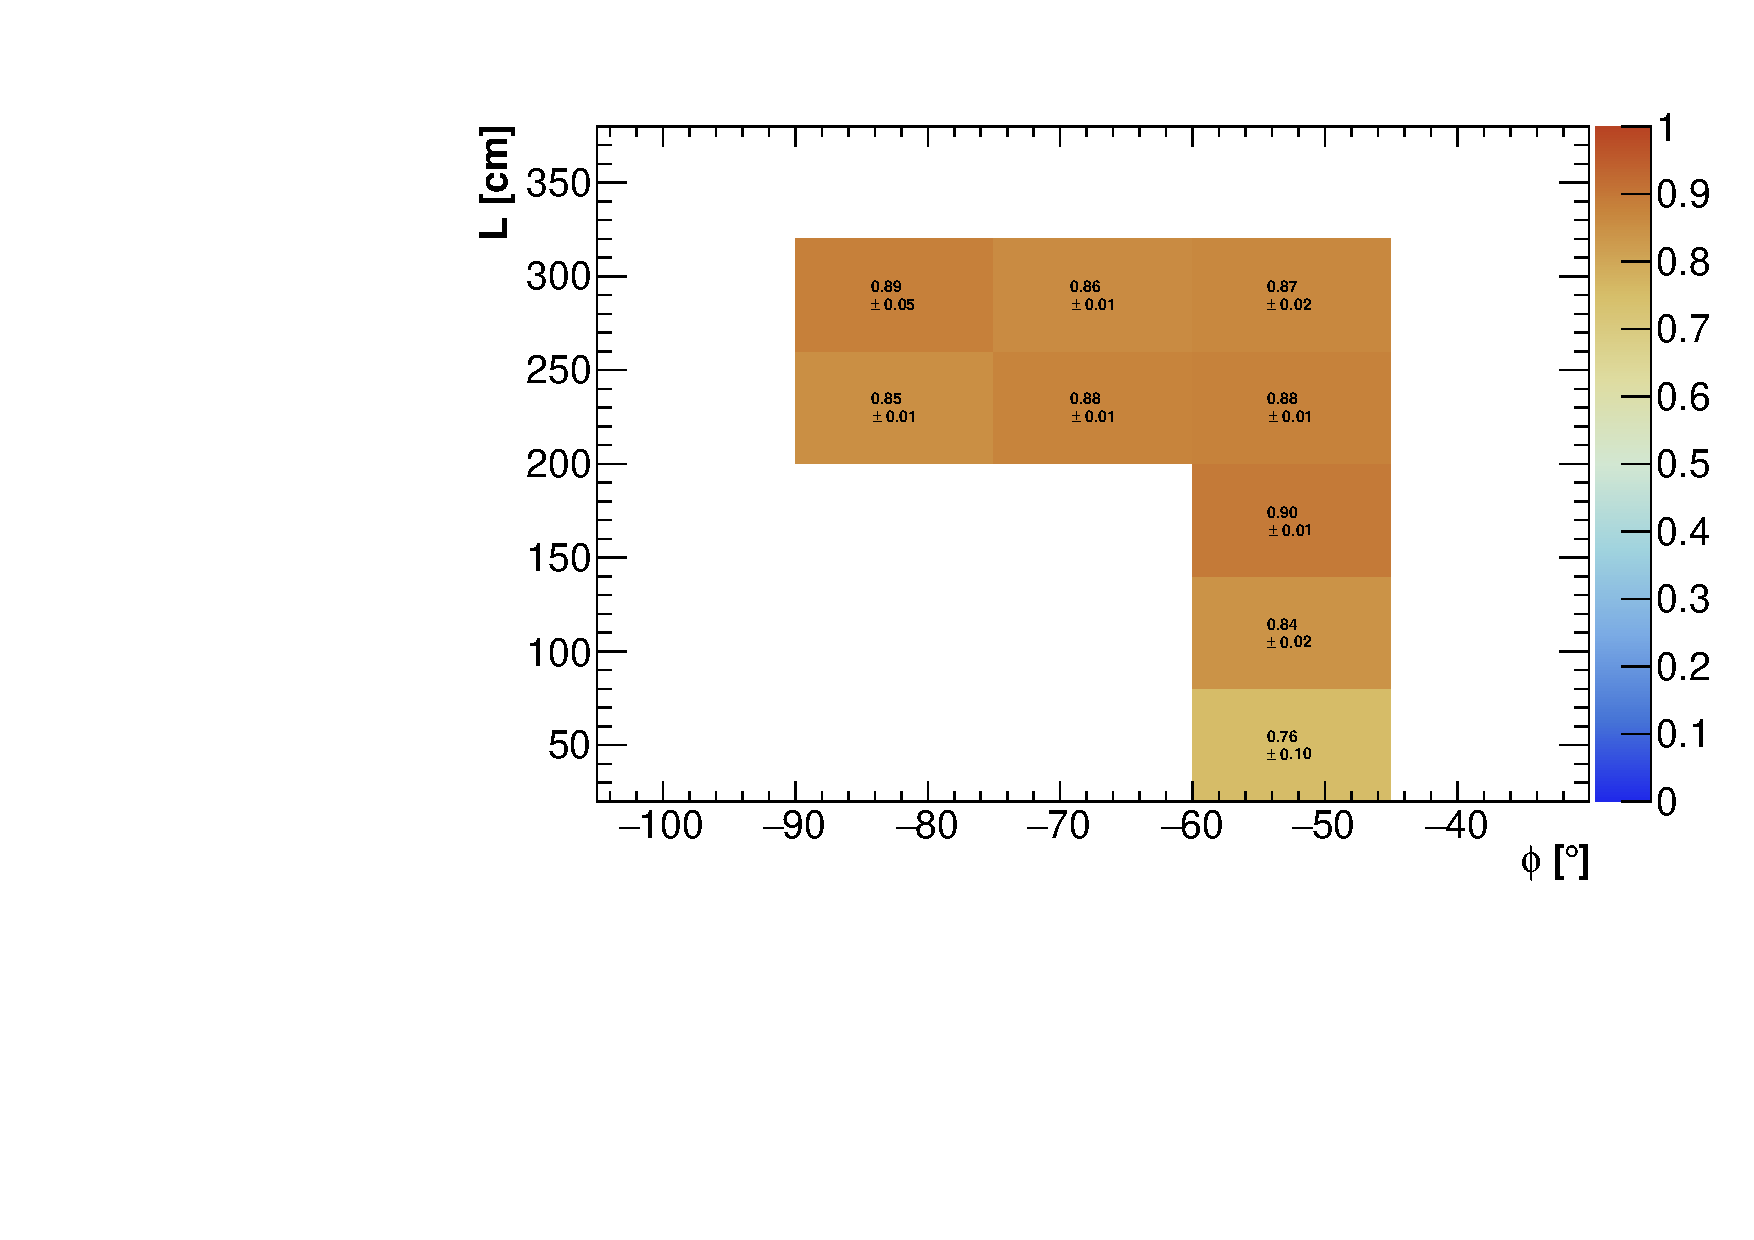
\includegraphics[width=\linewidth]{figures/phi_l_mc.pdf}
    \caption{$\phi - L$, Monte Carlo}\label{fig:2d_cry_mc_3}
  \end{subfigure}
  \begin{subfigure}{0.52\textwidth}
    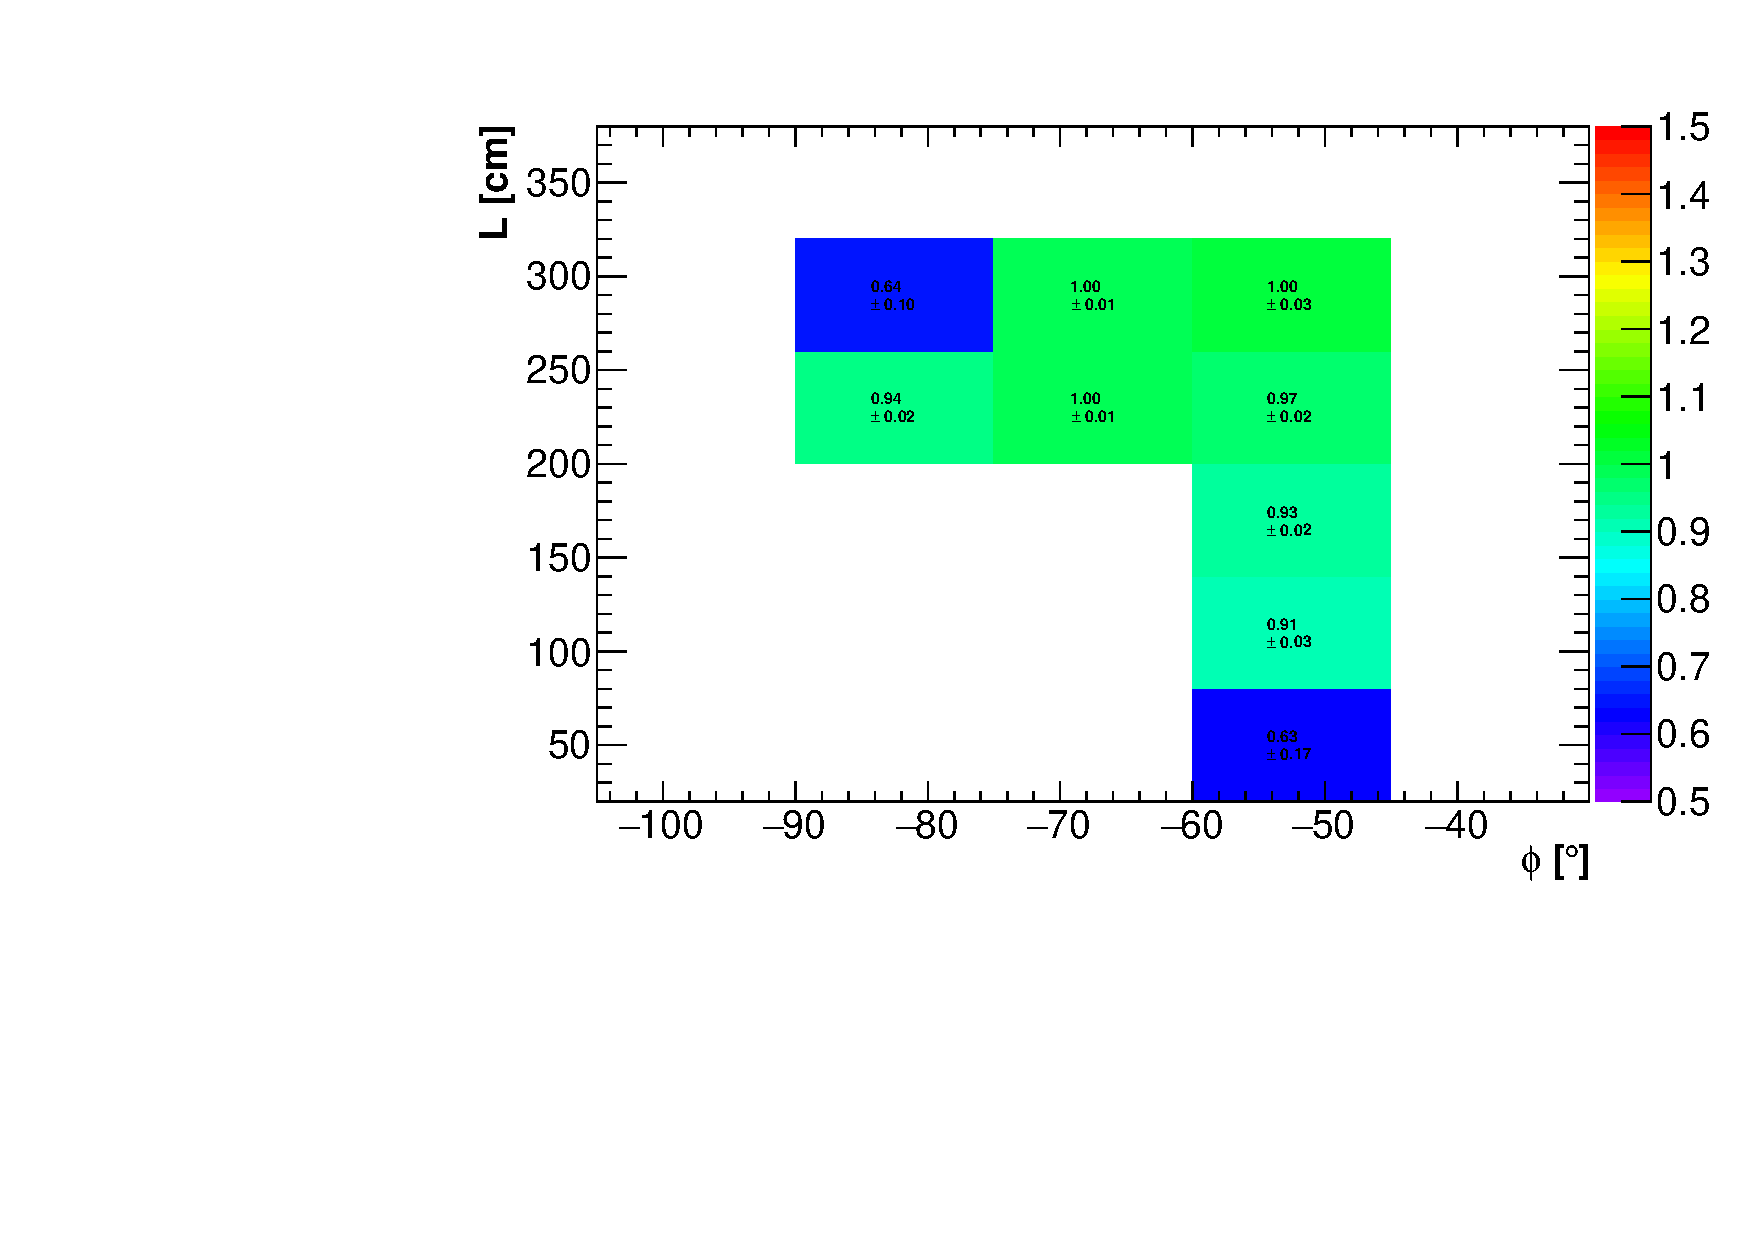
\includegraphics[width=\linewidth]{figures/ratio_phi_l.pdf}
    \caption{$\phi - L$, data/Monte Carlo}\label{fig:2d_cry_ratio_3}
  \end{subfigure}
  \caption{2D $\phi - L$ efficiency with the \texttt{pandoraCosmic} algorithm for data, Monte Carlo and data/Monte Carlo ratio.} \label{fig:cry_mc_2d_3}
\end{center}
\end{figure}


\begin{figure}[htbp]
  \begin{center}
    \begin{subfigure}{0.52\textwidth}
      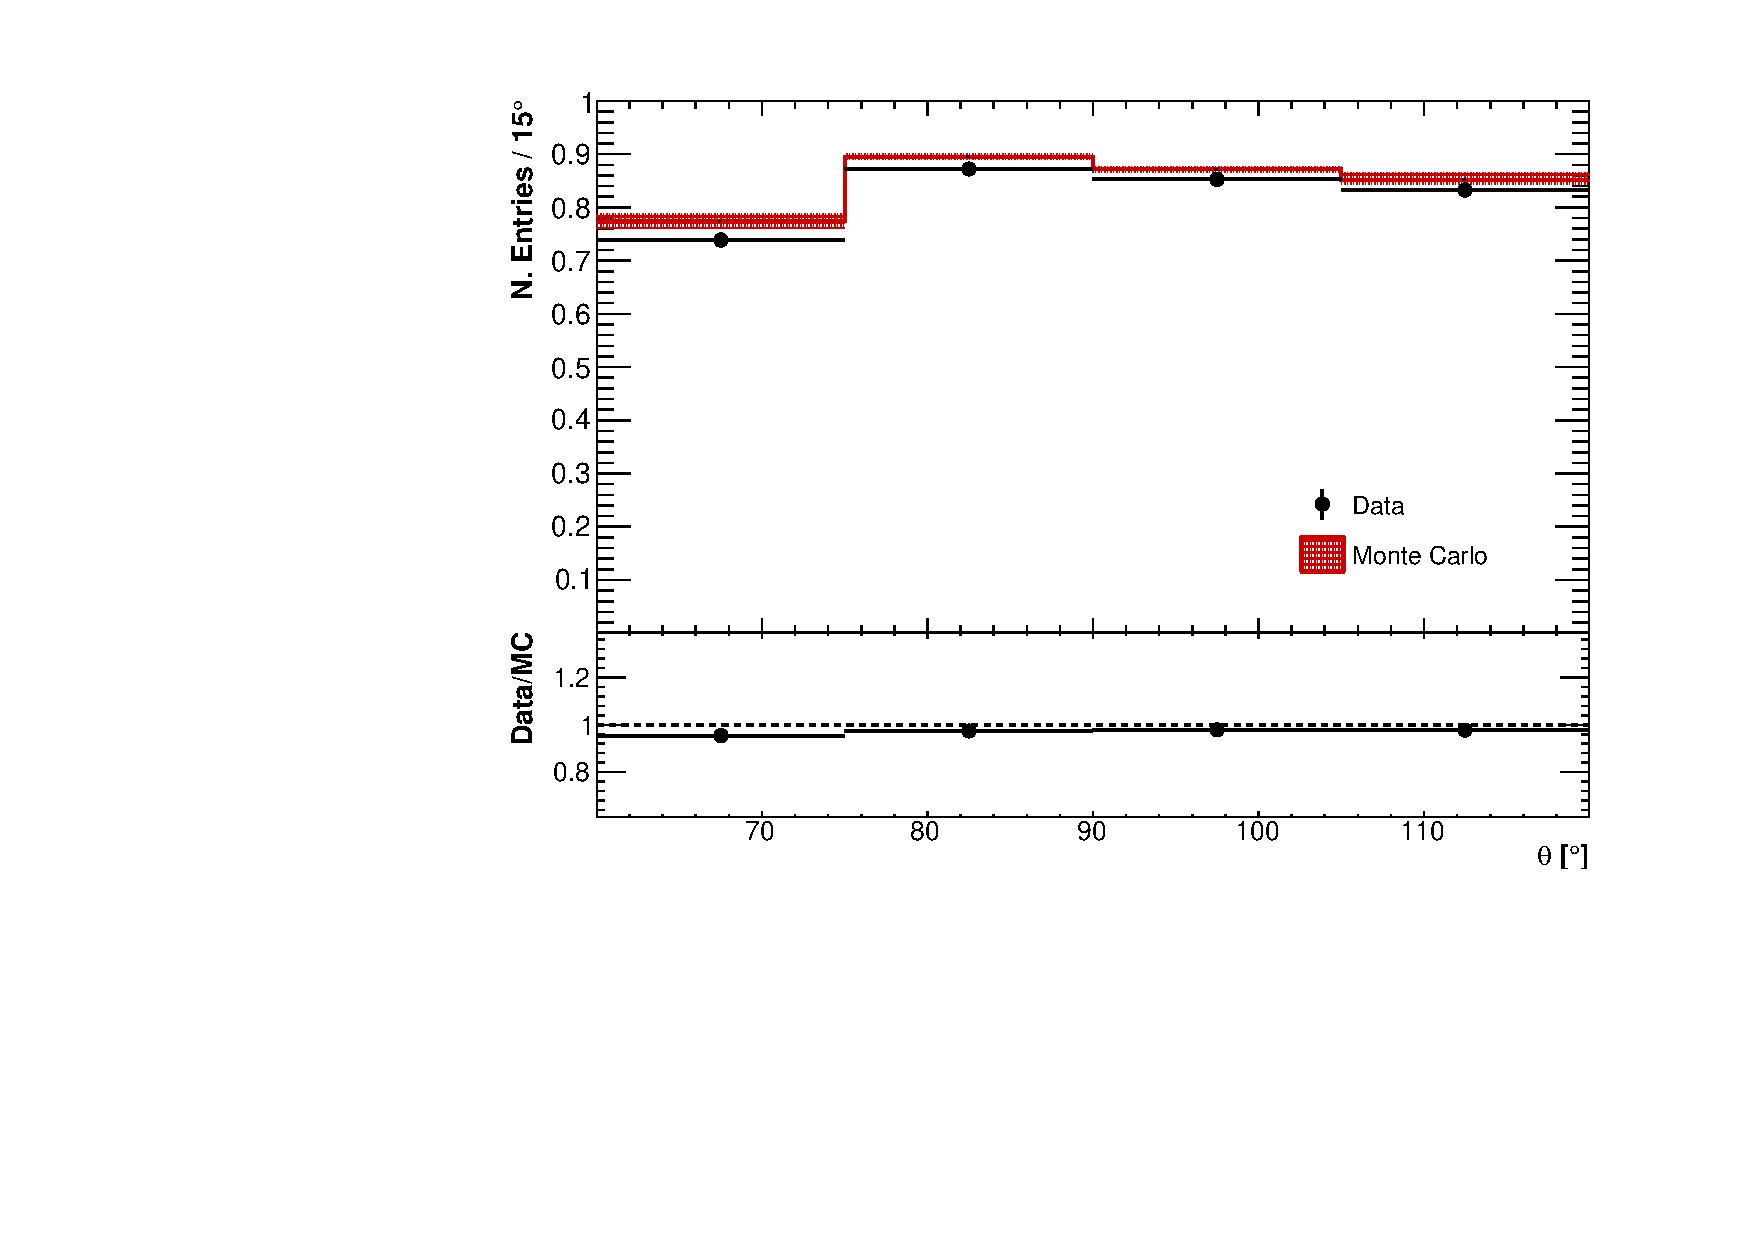
\includegraphics[width=\linewidth]{figures/theta_cry.pdf}
      \caption{$\theta$, data and Monte Carlo} \label{fig:1d_cry}
    \end{subfigure}\begin{subfigure}{0.52\textwidth}
    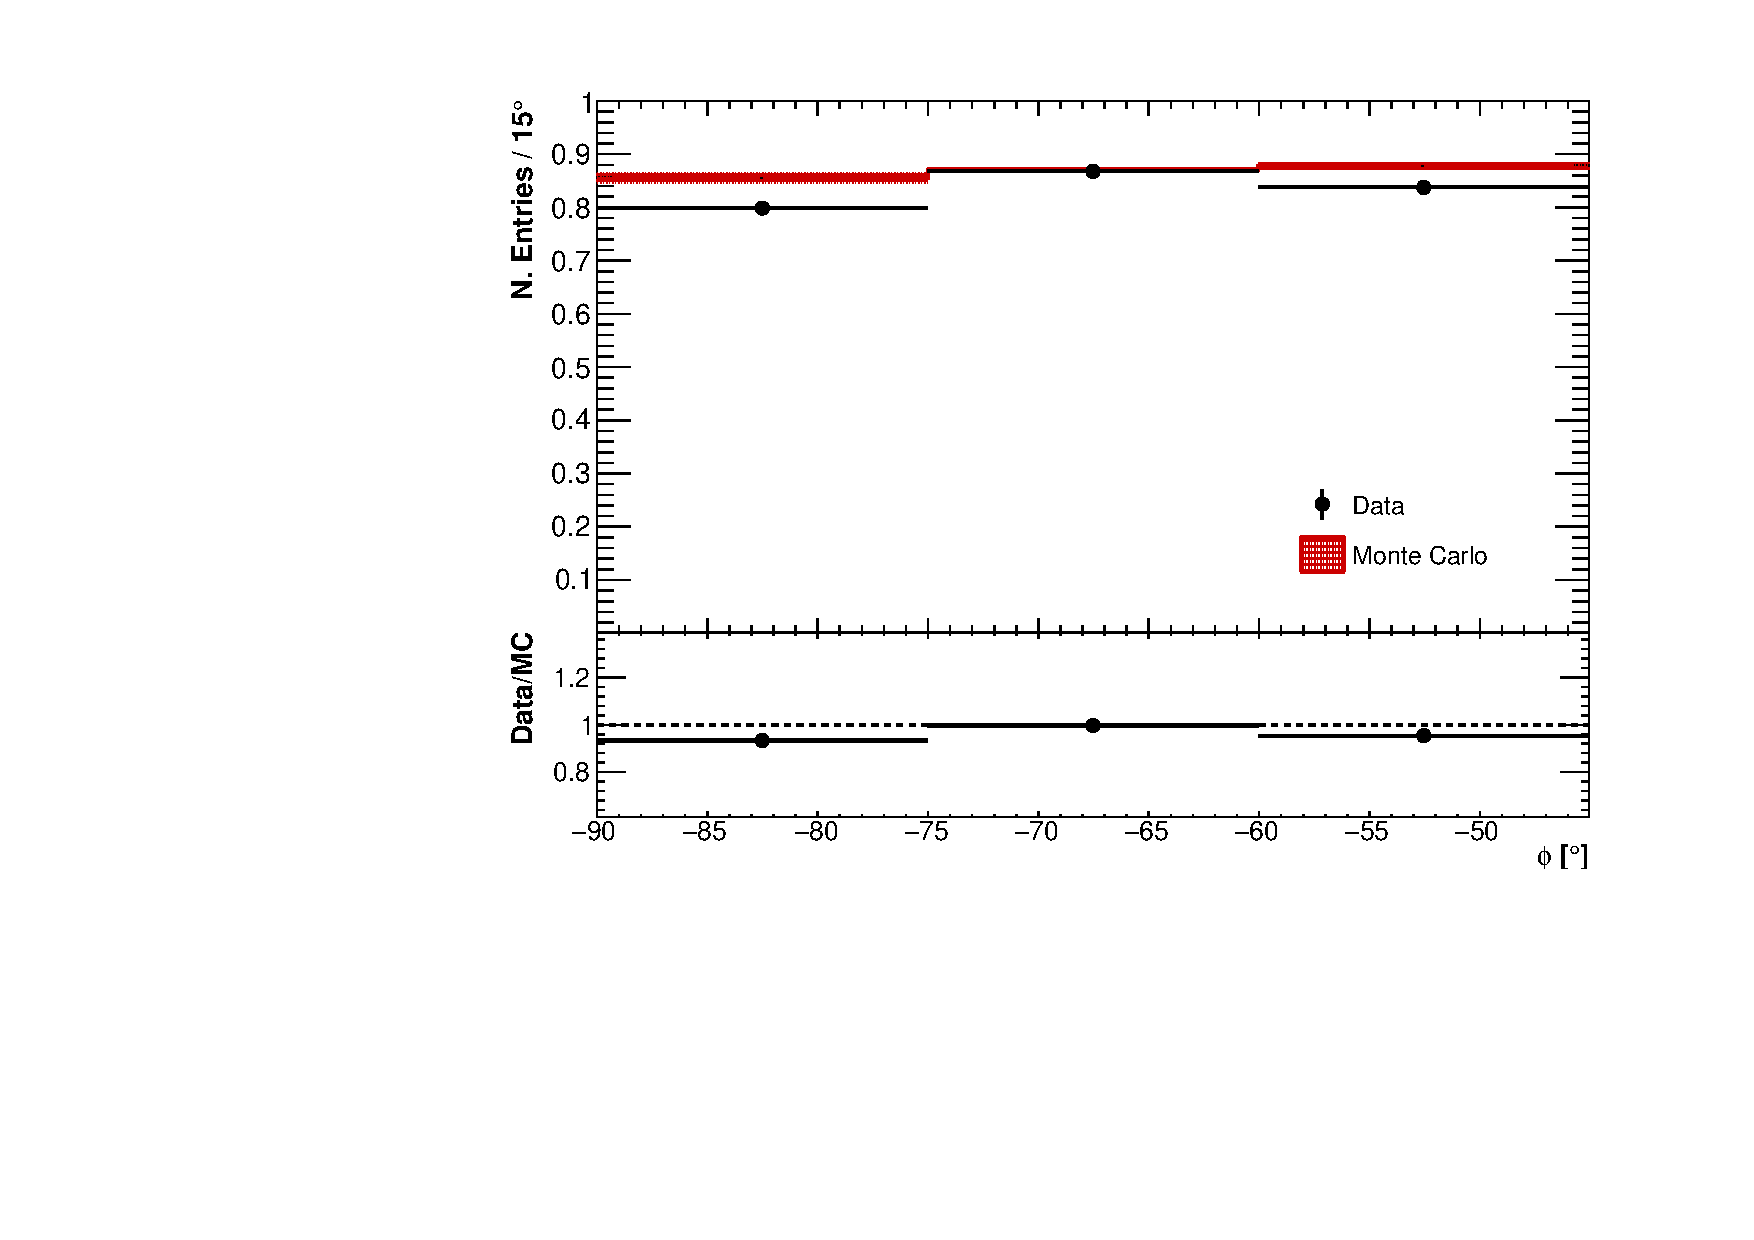
\includegraphics[width=\linewidth]{figures/phi_cry.pdf}
    \caption{$\phi$, data and Monte Carlo}\label{fig:1d_cry_mc}
  \end{subfigure}
  \begin{subfigure}{0.52\textwidth}
    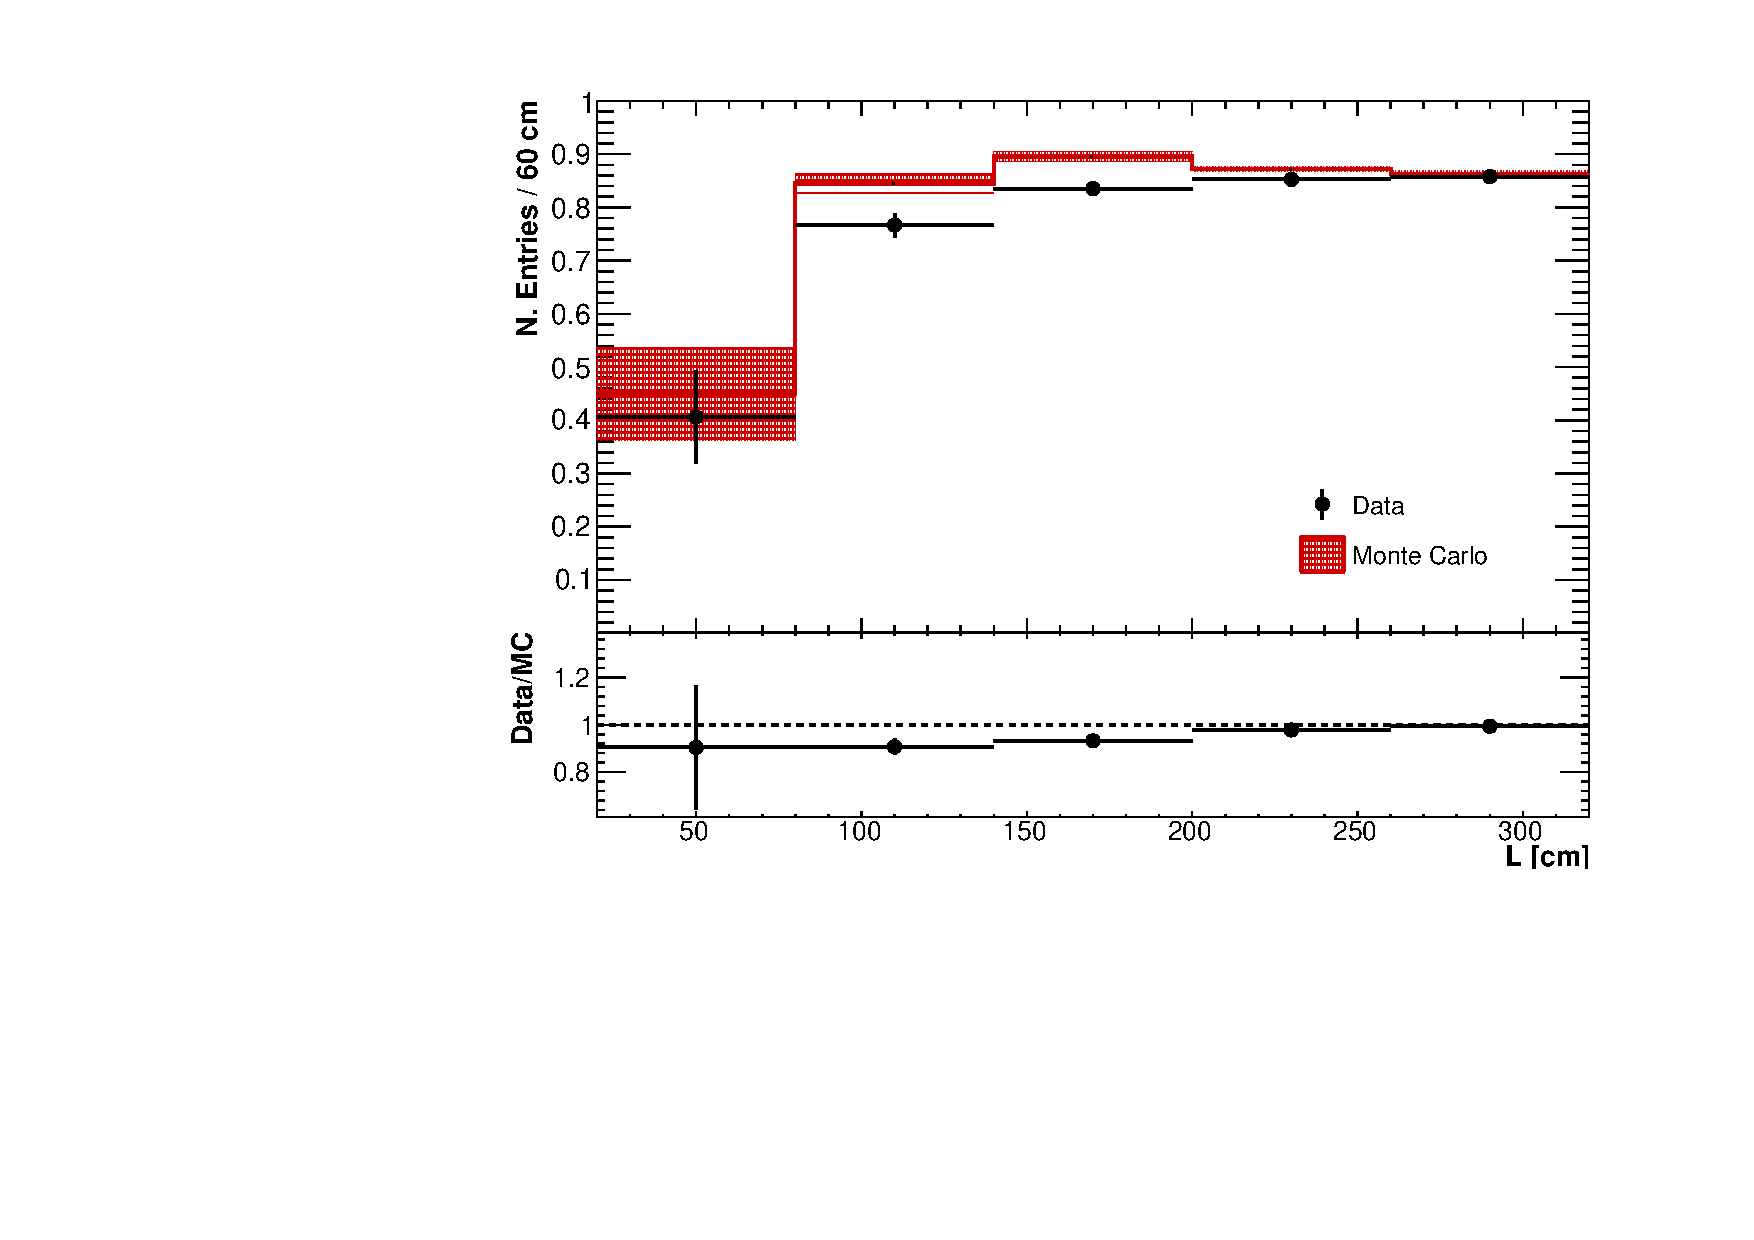
\includegraphics[width=\linewidth]{figures/l_cry.pdf}
    \caption{$L$, data and Monte Carlo}\label{fig:1d_cry_ratio}
  \end{subfigure}
  \caption{1D efficiencies with the \texttt{pandoraCosmic} algorithm for data and Monte Carlo.} \label{fig:cry_mc_1d}
\end{center}
\end{figure}

\clearpage{}

\section{Summary and plans}
We compared the data/Monte Carlo reconstruction efficiencies for cosmic rays  with three different algorithms, as a function of the starting angle and the path length of the cosmic rays, using a dataset of events triggered by the MuCS. We showed that the Monte Carlo reconstruction efficiency is energy-dependent and, in particular, lower energy cosmic rays correspond to a lower reconstruction efficiency. The Monte Carlo efficiency obtained with a CRY sample is in good agreement with the data.  Leftover discrepancies can be caused by (1) differences between the CRY energy spectrum and data energy spectrum and (2) absence of not-MuCS cosmic rays in the Monte Carlo sample.

By moving the MuCS boxes it is possible to increase the coverage of $(\theta_{xy}, \theta_{yz}, L)$ parameter space.
Our plan is to move the boxes at the center of the TPC on the $z$ axis. Then, the boxes will be aligned in the $x$ direction and their distance in the $y$ will be reduced, in order to cover the region with $\theta_{xy} = 90^{\circ}$, $\theta_{yz} < -120^{\circ}$ and $\theta_{yz} > -60^{\circ}$, as shown in Fig. \ref{fig:plans}.

\begin{figure}[htbp]
  \begin{center}
    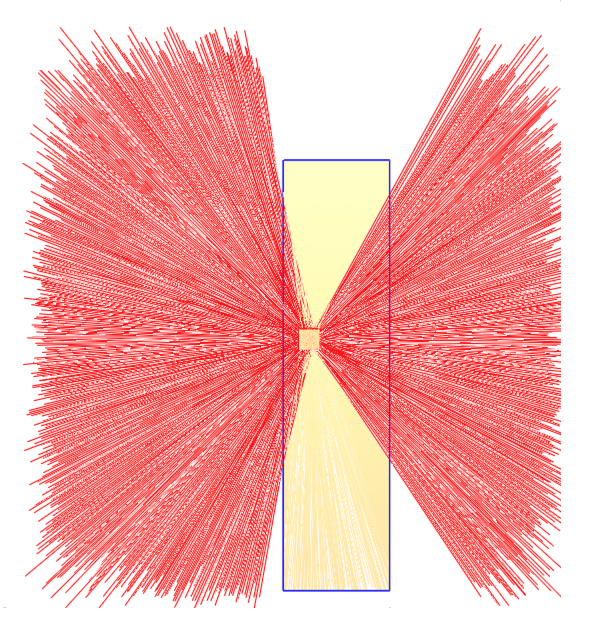
\includegraphics[width=0.3\linewidth]{figures/image.png}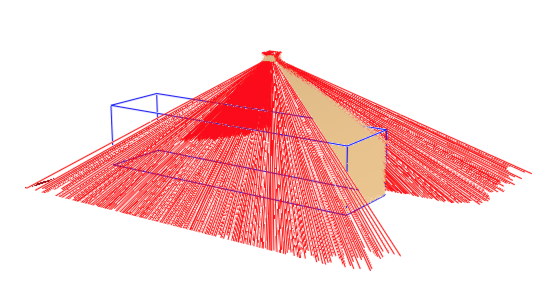
\includegraphics[width=0.65\linewidth]{figures/image2.png}
  \end{center}
  \caption{Monte Carlo simulation of the planned new positioning of the MuCS. Red lines show cosmic rays that trigger the MuCS but don't hit the TPC.}\label{fig:plans}
\end{figure}

Once we have obtained a larger coverage of the $(\theta_{xy}, \theta_{yz}, L)$ parameter space, it will be possible to measure the efficiency-corrected cosmic-ray flux on the top of the TPC, both for data and Monte Carlo. Moreover, testing different regions of the TPC will allow us to measure eventual systematic errors caused by detector non-uniformity.

\appendix

\section{500 MeV Monte Carlo sample}\label{sec:500mev}
In order to check if the differences observed between data and Monte Carlo are caused by the energy of the Monte Carlo cosmic rays, we generated a sample of 500 MeV cosmic muons and measured the efficiency in the same way described in Sec. \ref{sec:proc}. The efficiency plots, for \texttt{pandoraCosmic} only, are shown in Fig. \ref{fig:500mev2d} and \ref{fig:500mev1d}. The integrated efficiency in this case is $(81.4 \pm 0.4) \%$, to be compared with $(96.5 \pm 0.2) \%$, obtained with the 4 GeV sample.

We can then safely assume that the reconstruction efficiency is proportional to the cosmic-ray energy, since cosmic rays with lower energy scatter more in the liquid argon and their track then more difficult to reconstruct.

\begin{figure}[htbp]
  \begin{subfigure}{0.52\textwidth}
    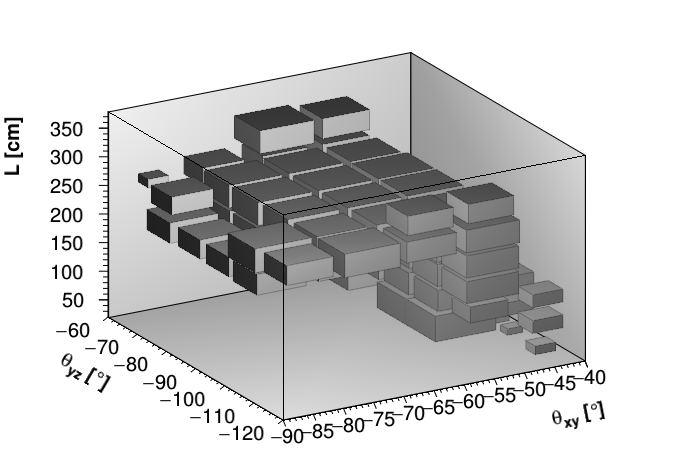
\includegraphics[width=\linewidth]{figures/pandora_500mev_mc.png}
    \caption{3D Monte Carlo efficiency with \texttt{pandoraCosmic}.}\label{fig:pandora_3D_mc_500}
  \end{subfigure}
  \begin{subfigure}{0.52\textwidth}
    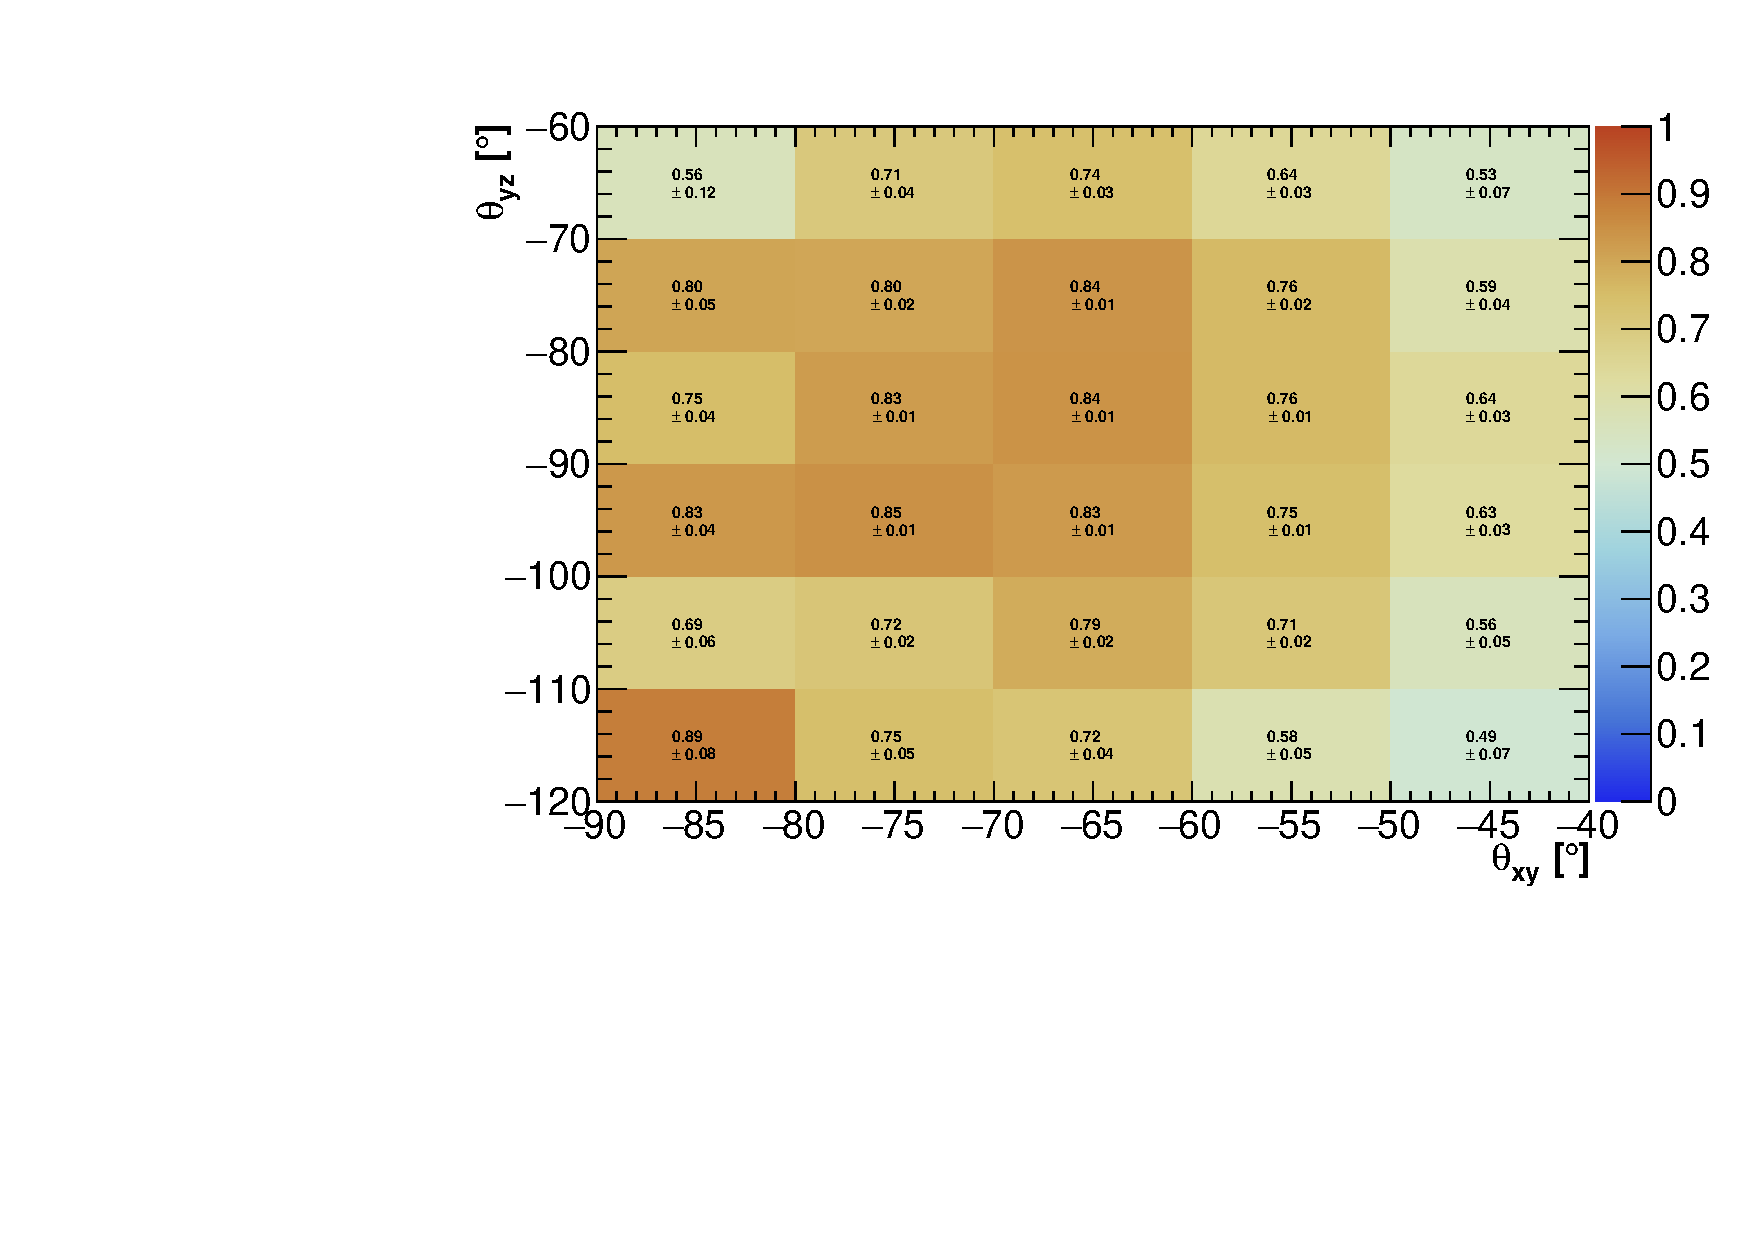
\includegraphics[width=\linewidth]{figures/e_xy_yz_500mev_mc.pdf}
    \caption{$\theta_{xy} - \theta_{yz}$, \texttt{pandoraCosmic} - Monte Carlo}\label{fig:5001d_pc1_mc}
  \end{subfigure}
  \begin{subfigure}{0.52\textwidth}
    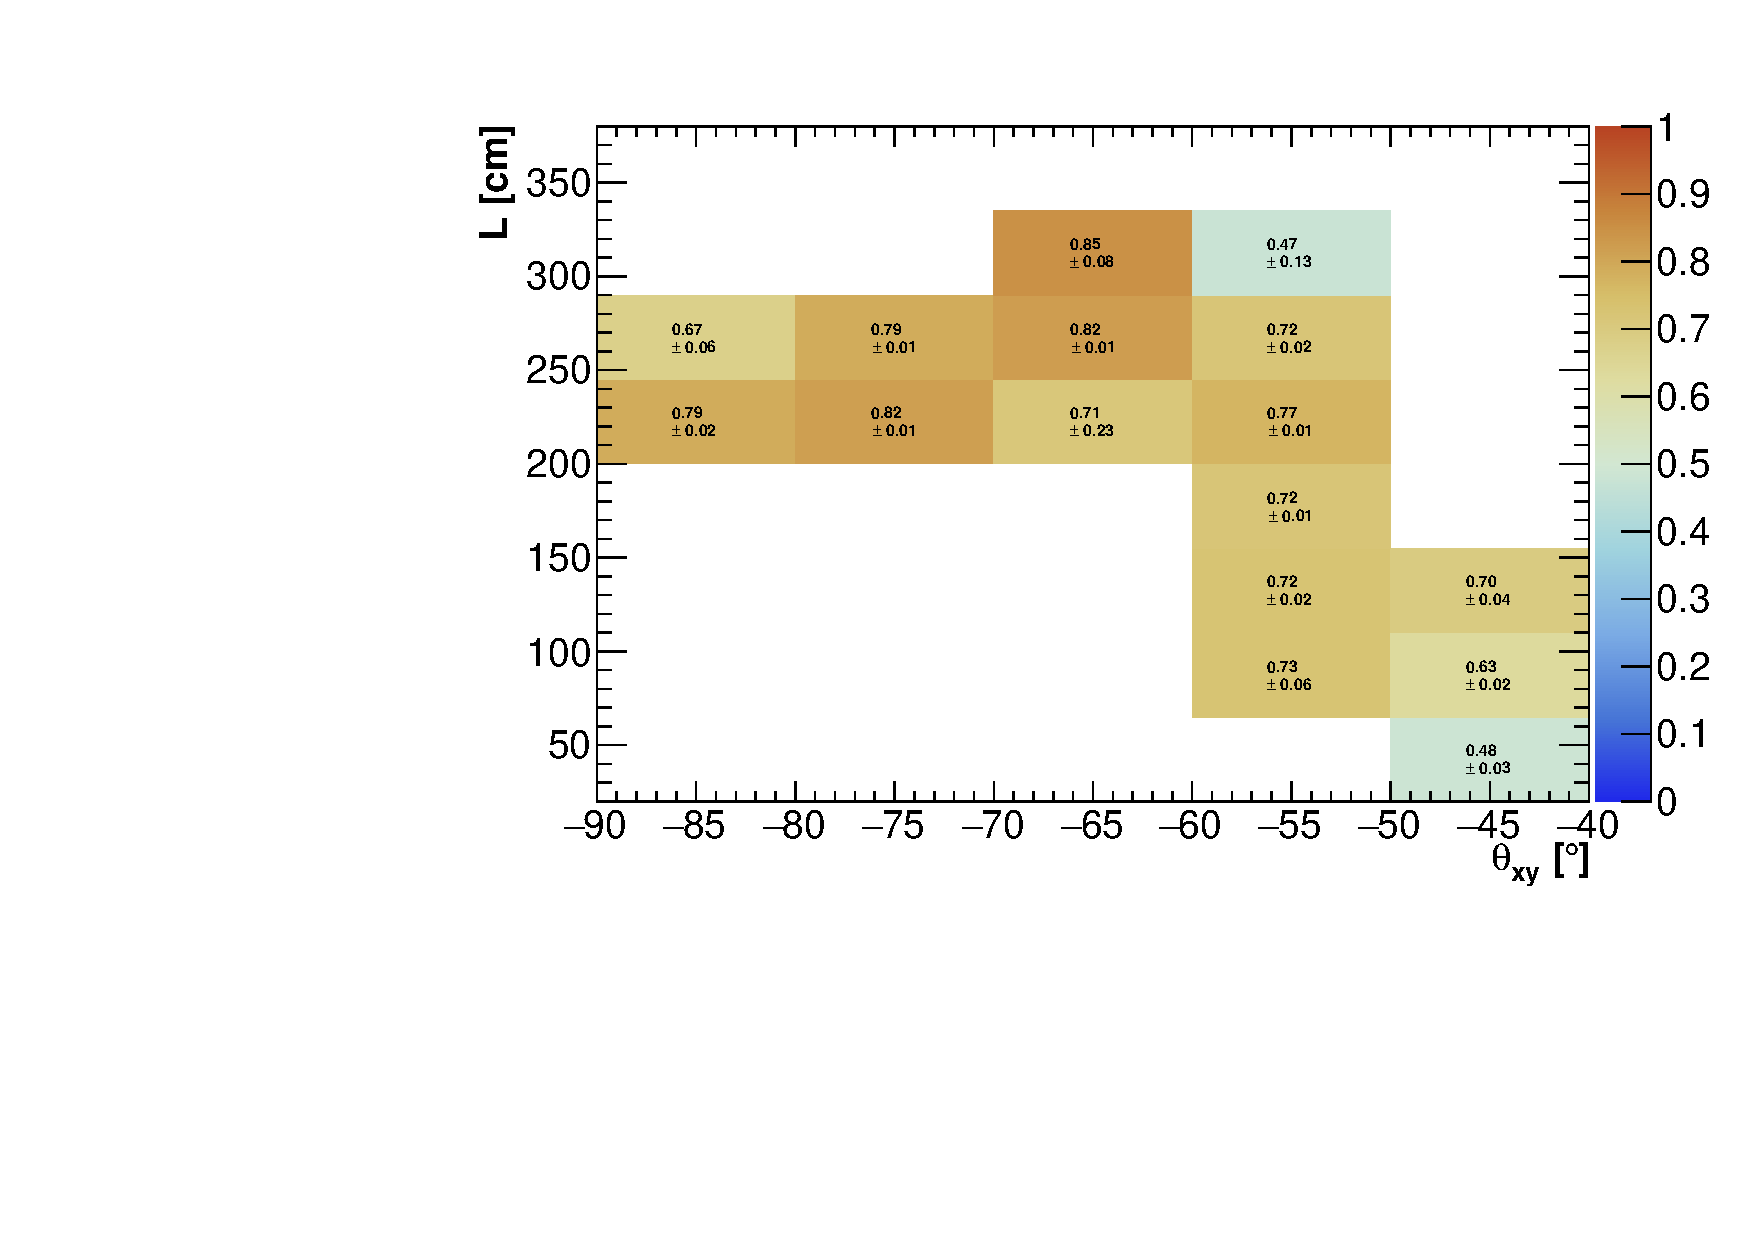
\includegraphics[width=\linewidth]{figures/e_xy_l_500mev_mc.pdf}
    \caption{$\theta_{xy} - L$, \texttt{pandoraCosmic} - Monte Carlo}\label{fig:5001d_pc2_mc}
  \end{subfigure}
  \begin{subfigure}{0.52\textwidth}
    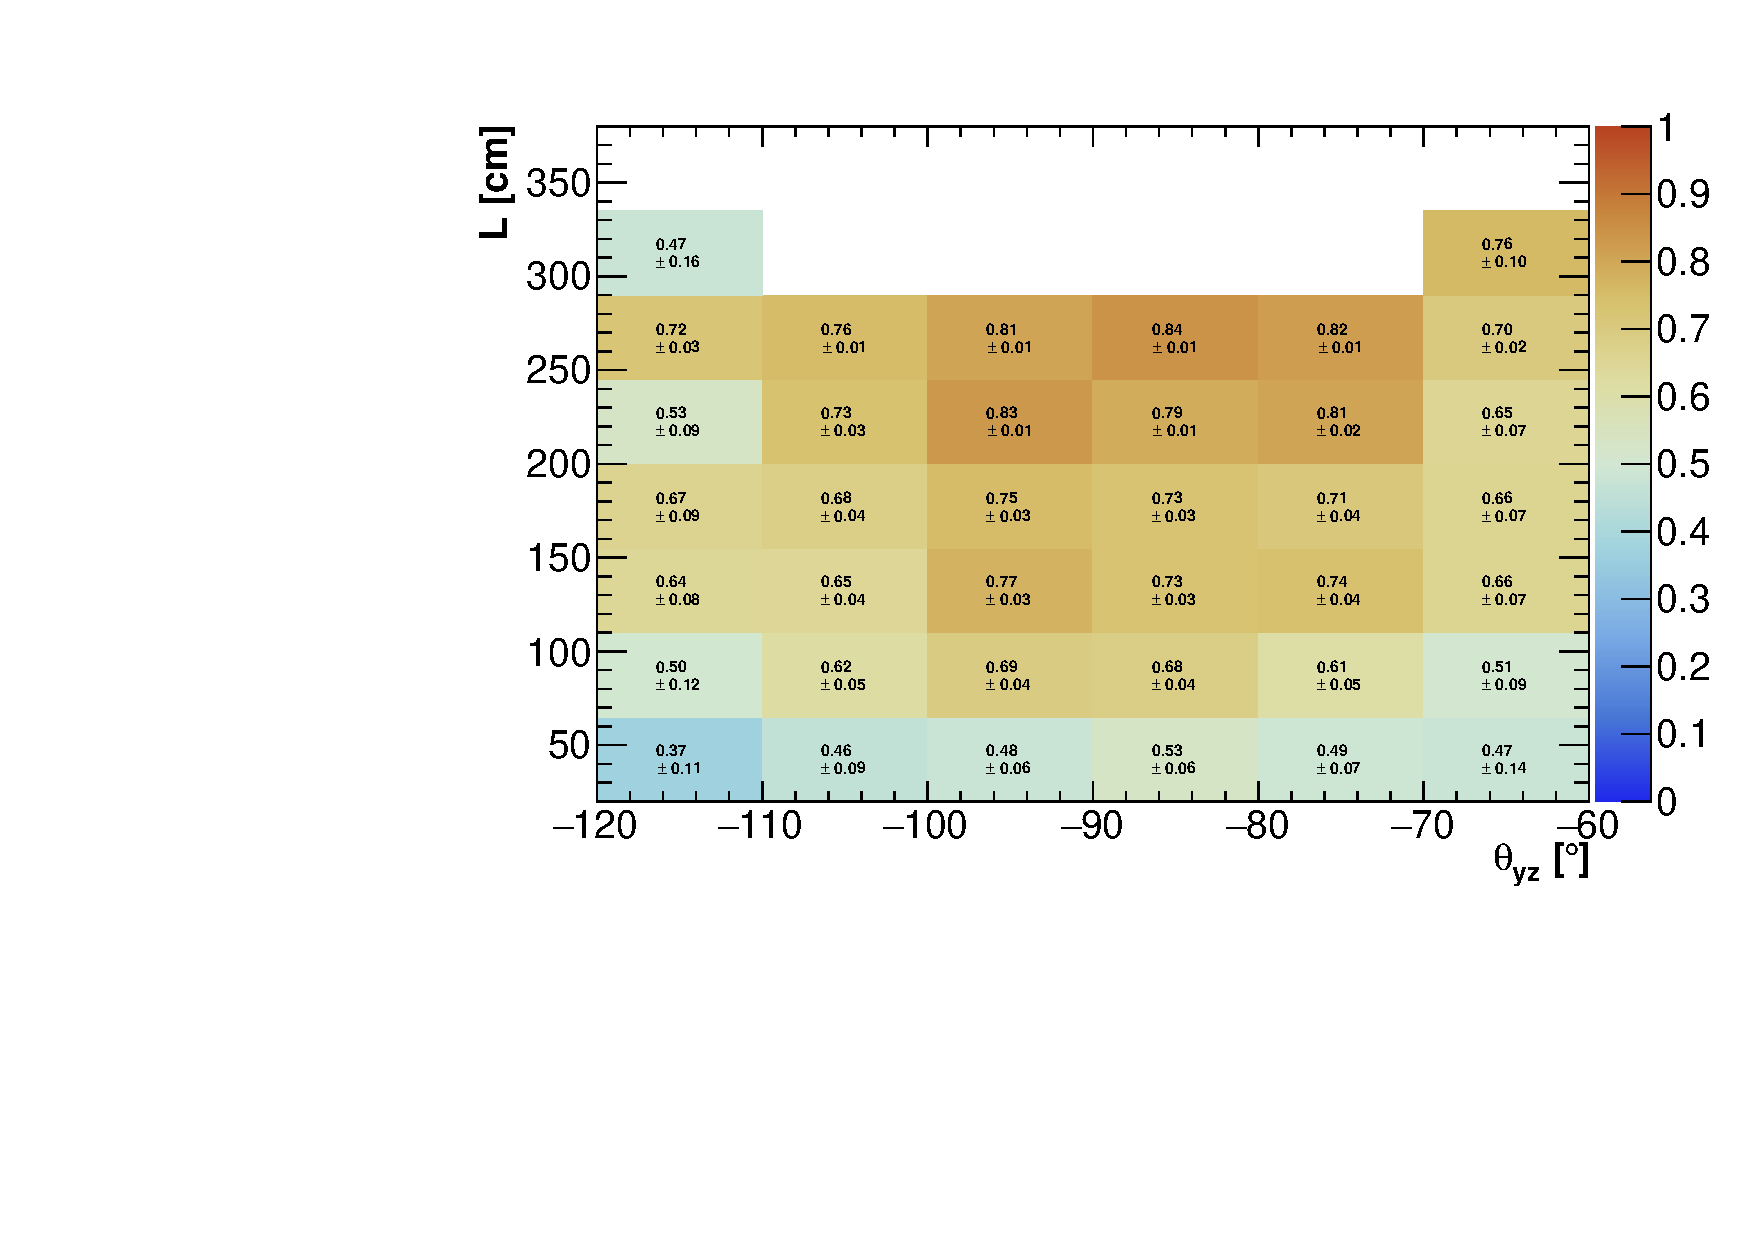
\includegraphics[width=\linewidth]{figures/e_yz_l_500mev_mc.pdf}
    \caption{$\theta_{yz} - L$, \texttt{pandoraCosmic} - Monte Carlo}\label{fig:5001d_pc3_mc}
  \end{subfigure}
  \caption{3D reconstruction efficiency (top-left) and 2D scatter-plots for the 500 MeV Monte Carlo \texttt{pandoraCosmic} algorithm.} \label{fig:500mev2d}
\end{figure}

\begin{figure}[htbp]
  \begin{center}
    \begin{subfigure}{0.55\textwidth}
      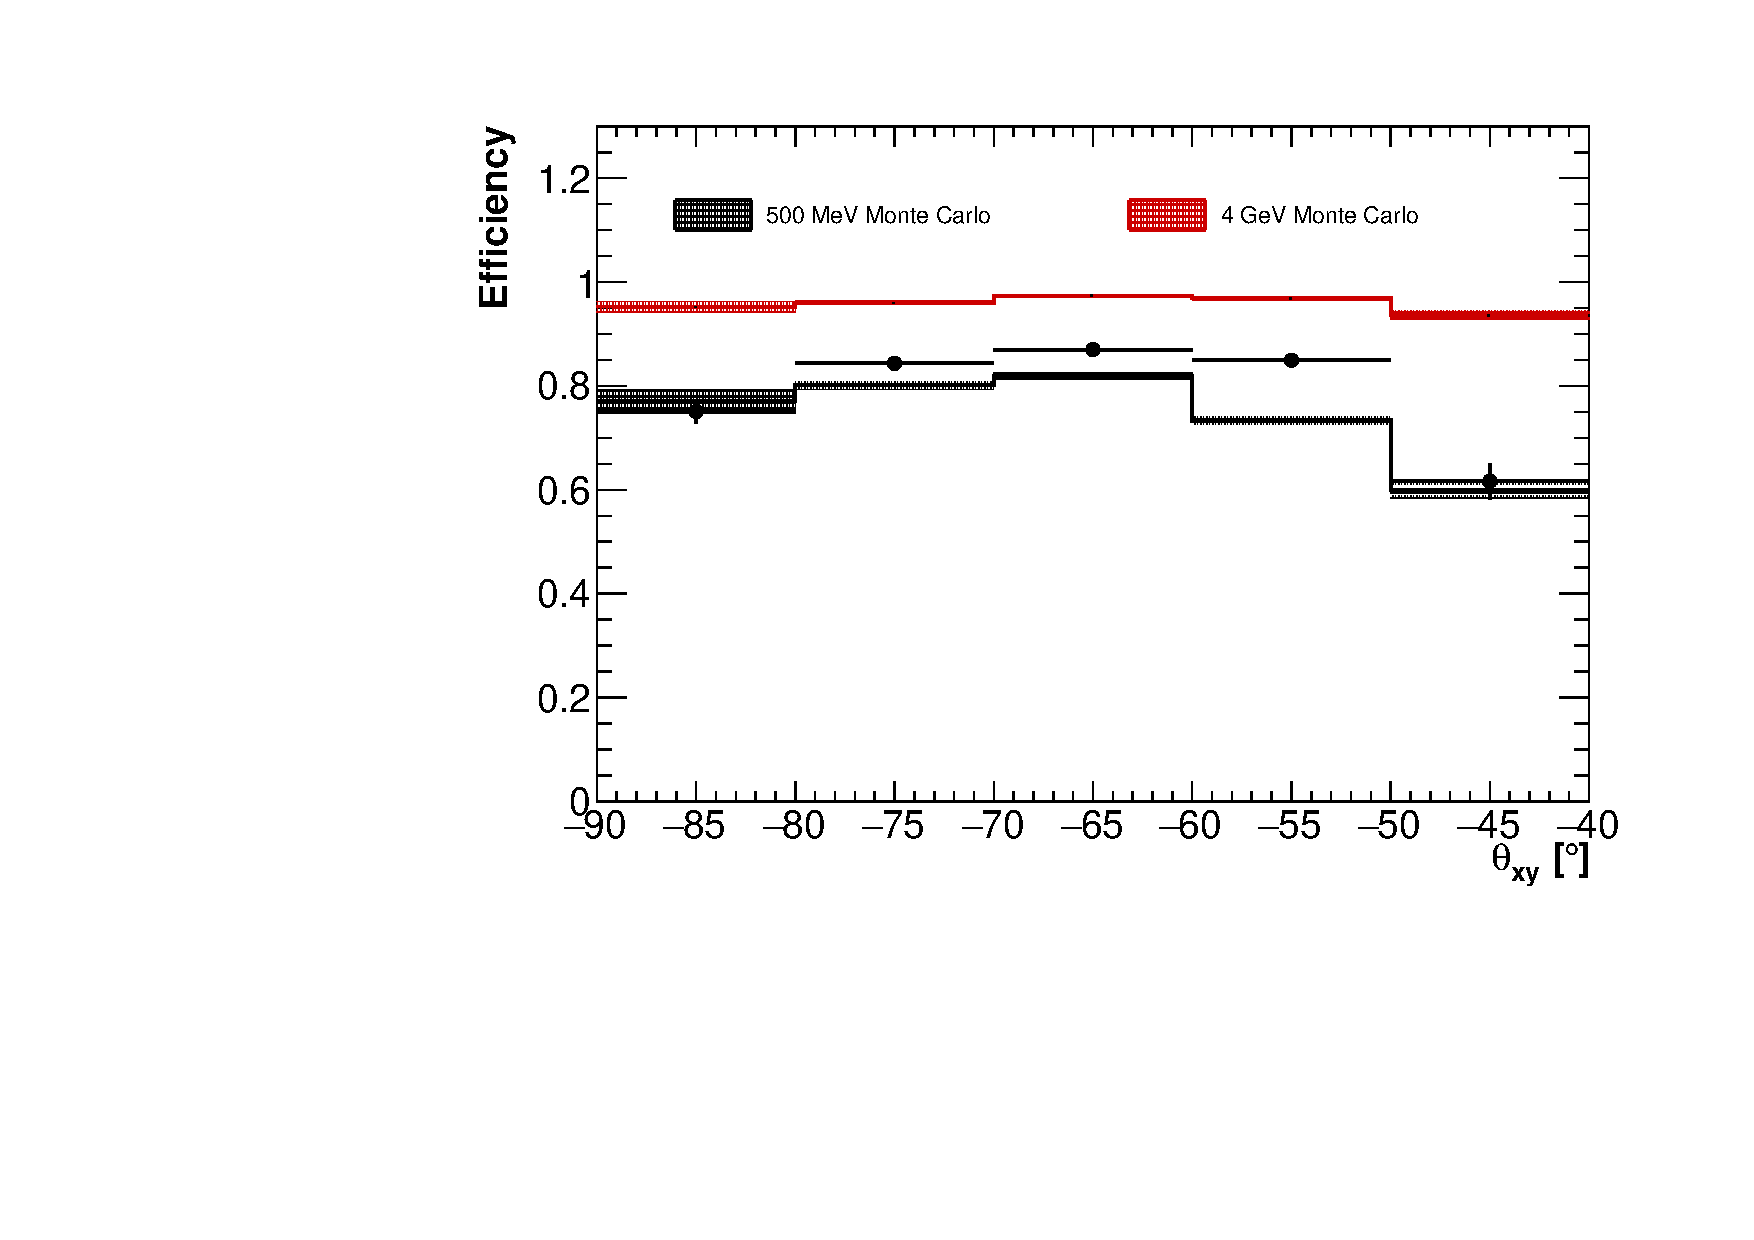
\includegraphics[width=\linewidth]{figures/xy_500.pdf}
      \caption{Efficiency as a function of $\theta_{xy}$.} \label{fig:xy_500}
    \end{subfigure}\begin{subfigure}{0.55\textwidth}
    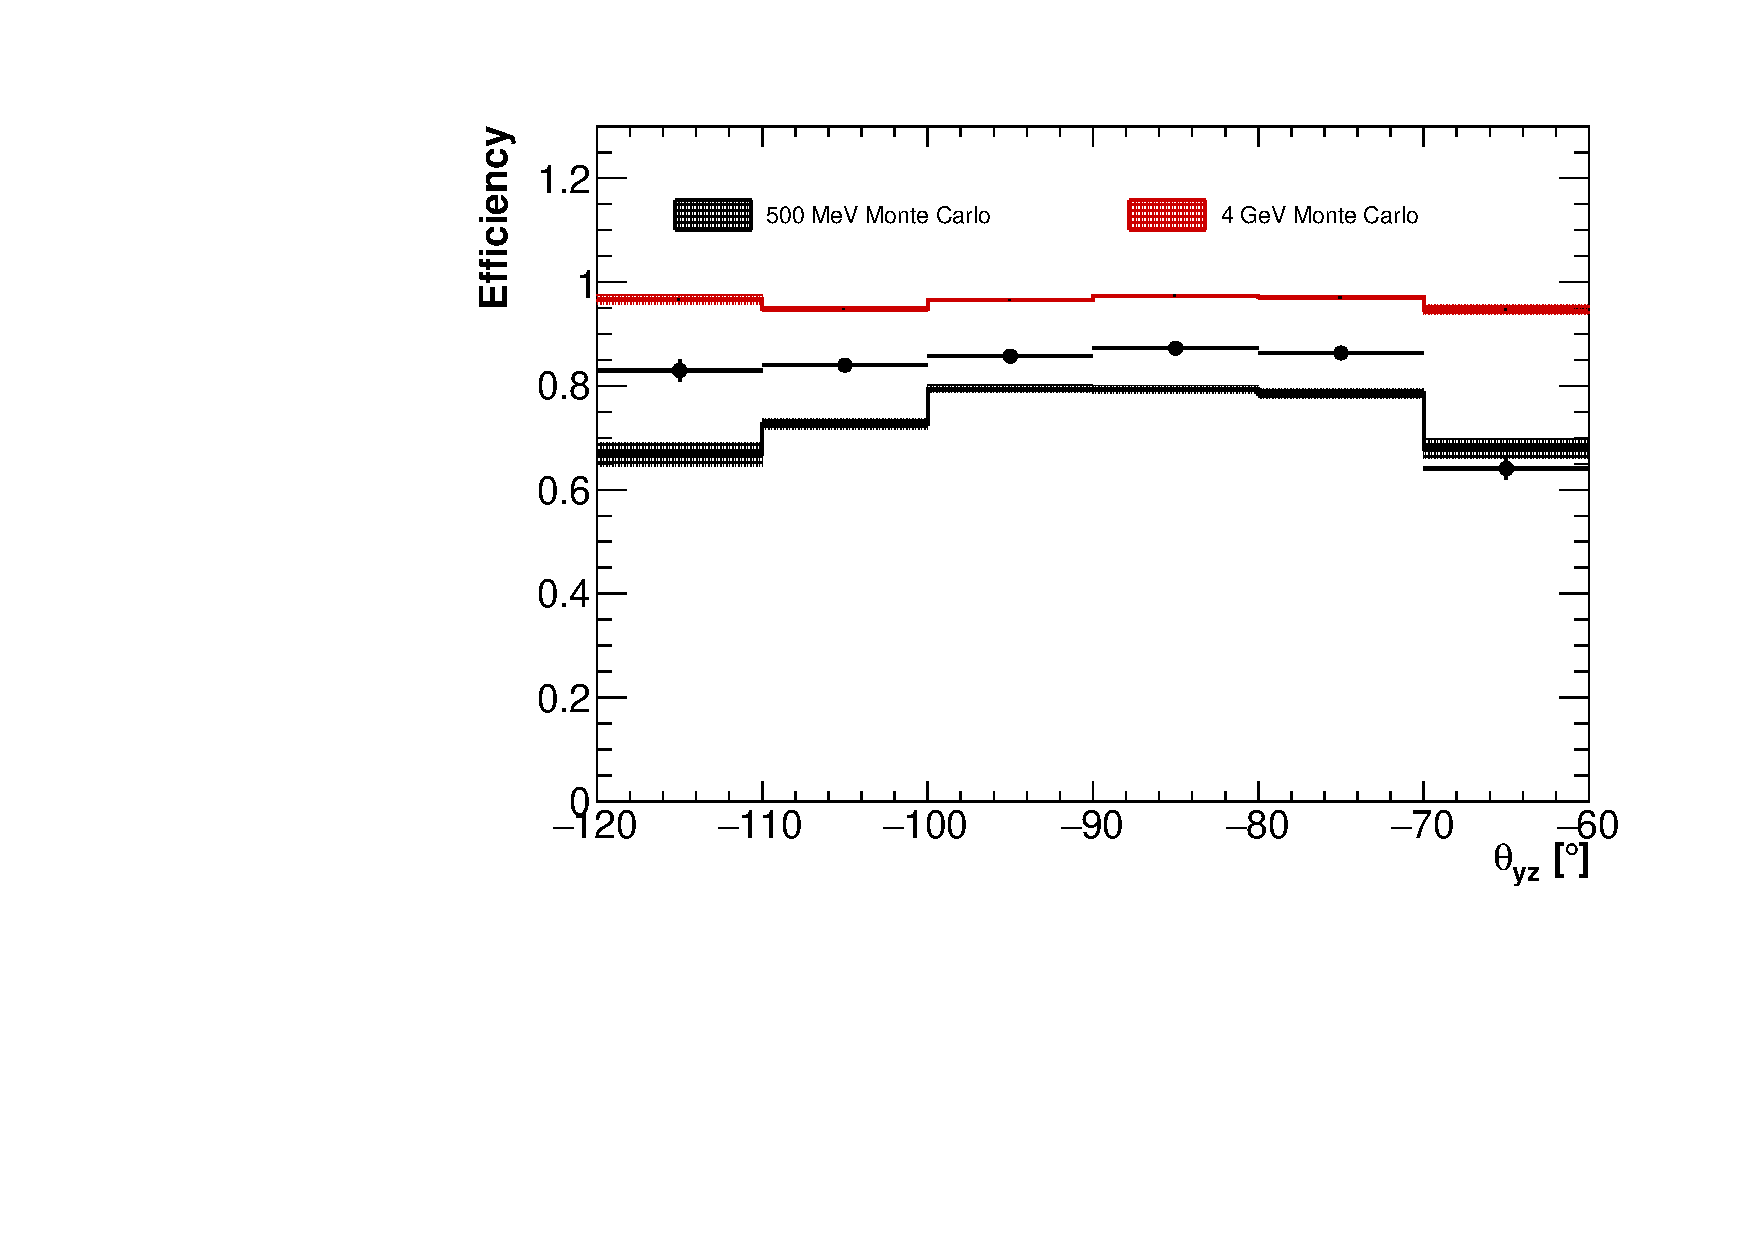
\includegraphics[width=\linewidth]{figures/yz_500.pdf}
    \caption{Efficiency as a function of $\theta_{yz}$}\label{fig:yz_500}
  \end{subfigure}
  \begin{subfigure}{0.55\textwidth}
    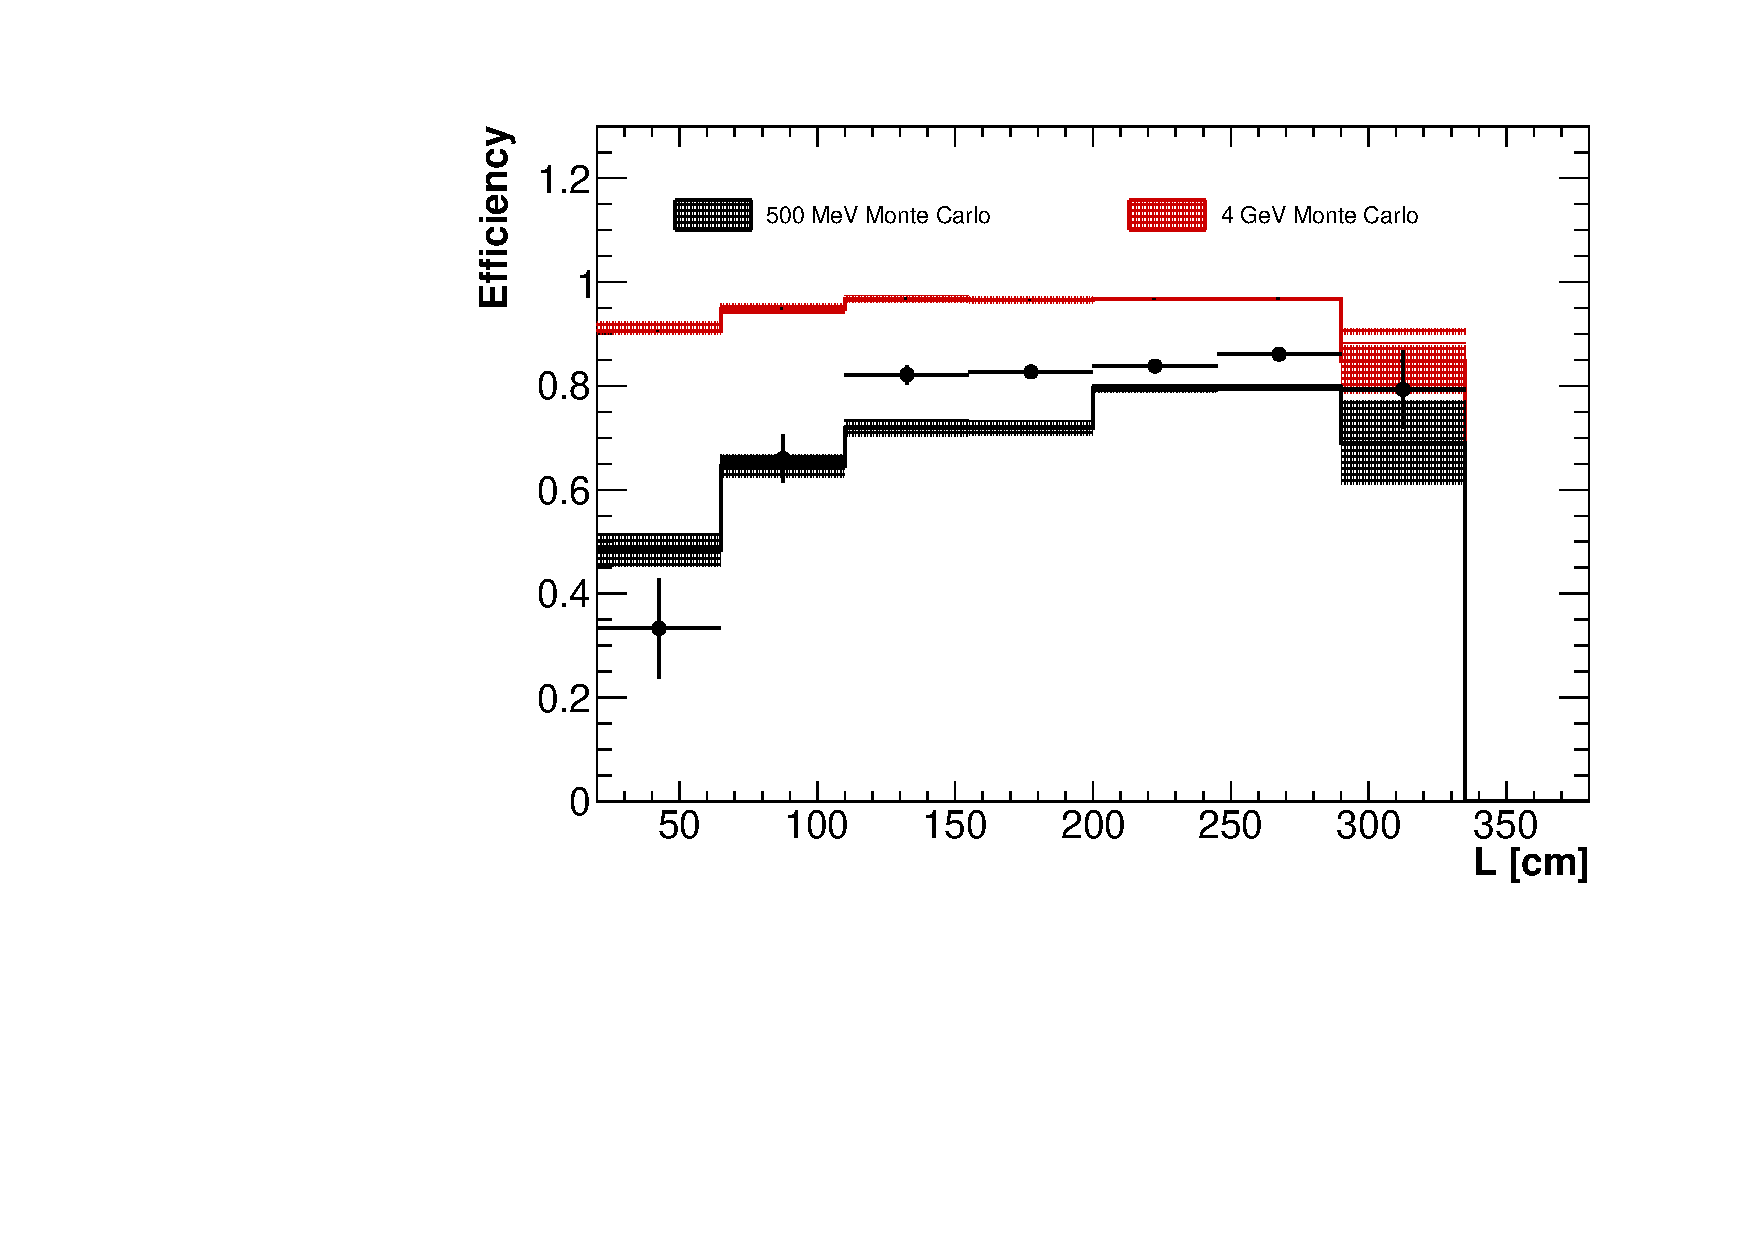
\includegraphics[width=\linewidth]{figures/l_500.pdf}
    \caption{Efficiency as a function of $L$}\label{fig:l_500}
  \end{subfigure}
  \caption{Monte Carlo efficiencies with the 500 MeV (black) and 4 GeV (red) samples, as a function of $\theta_{xy}$, $\theta_{yz}$ and $L$ for the \texttt{pan\-do\-ra\-Co\-smic} reconstruction algorithms.} \label{fig:500mev1d}
\end{center}
\end{figure}

\clearpage{}
\section{Technical details}
The dataset used in this analysis correspond to run 3702 and run 7106. The reconstruction stages \texttt{reco1} and \texttt{reco2} use \texttt{uboonecode v05\_08\_00}. Their configuration is provided by the standard fcl files \texttt{reco\_uboone\_mcc7\_driver\_stage1.fcl} and \texttt{reco\_uboone\_mcc7\_driver\_stage2.fcl}. The source code of the \texttt{MuCSMerger} and \texttt{MuCSTagger} modules is available on the \texttt{uboonecode} repository.

The dataset with the merged MuCS, Monte Carlo and data information are stored in \texttt{/uboone/data/users/mibass/MuCS/MuCS/v05\_08\_00/MergedOuttree/}.


\begin{thebibliography}{9}

  \bibitem{pandoracosmic} R. Acciarri, et al. [MicroBooNE Collaboration], \textit{The Pandora multi-algorithm approach to automated pattern recognition in LAr TPC detectors}. \texttt{MICROBOONE- NOTE-1015-PUB}, 2016. \url{http://www-microboone.fnal.gov/publications/publicnotes/index.html}.

  \bibitem{pandora} J.~S.~Marshall and M.~A.~Thomson, \textit{The Pandora Software Development Kit for Pattern Recognition}, Eur.\ Phys.\ J.\ C 75, no. 9, 439 (2015) \texttt{doi:10.1140/epjc/s10052\-015-3659-3} \texttt{[arXiv:1506.05348 [physics.data-an]]}.

  \bibitem{cosmic} R. Acciarri, et al. [MicroBooNE Collaboration], \textit{Cosmic Shielding Studies at MicroBooNE}. \texttt{MICROBOONE-NOTE-1005-PUB}, 2016. \url{http:// www-microboone.fnal.gov/publications/publicnotes/index.html}.

  \bibitem{crt} M. Auger, et al., \textit{A Novel Cosmic Ray Tagger System for Liquid Argon TPC Neutrino Detectors}, Instruments 2016, 1, 1.

  \bibitem{mcdata} R. Acciarri, et al. [MicroBooNE Collaboration], \textit{A Comparison of Monte-Carlo Simulations and Data from MicroBooNE}, \texttt{MICROBOONE-NOTE-1014-PUB}.

  \bibitem{corsika} D.~Heck, et al.,
  \textit{CORSIKA: A Monte Carlo code to simulate extensive air showers},
  \texttt{FZKA-6019}, 1998.

  \bibitem{geant} S.~Agostinelli, et al. [GEANT4 Collaboration], \textit{GEANT4: A Simulation toolkit}, Nucl.\ Instrum.\ Meth.\ A {506}, 250 (2003).

  \bibitem{sce} R. Acciarri, et al. [MicroBooNE Collaboration], \textit{Space Charge Effect Measurements and Corrections}. \texttt{MICROBOONE-NOTE-1018-PUB}, 2016. \url{http: //www-microboone.fnal.gov/publications/publicnotes/index.html}.

  \bibitem{cry} C. Hagmann, et al., \textit{Cosmic-ray Shower Library (CRY)},  Lawrence Livermore National Laboratory, \texttt{UCRL-TM-229453}, 2012.


\end{thebibliography}

\end{document}
